\clearpage
\label{atlaspart:instruments}
\part*{Instruments}
\addcontentsline{toc}{part}{Instruments}
\setcounter{section}{0}
\renewcommand{\thesection}{I.\arabic{section}}
\section*{The instrument chapters}
\addcontentsline{toc}{section}{The instrument chapters}
Each Part lists its instrument chapters in its chapter titled \emph{The instrument tables of this Part}. They are printed here, in the order those chapters list them, with the comments removed as in the rest of this compendium. They are numbered I.1 to I.52, so that no number in the Parts changes. Each one names the Part that lists it.
\section{The Rosetta table in full}\label{mod:I-7-rosetta-table-in-full}
\chdesig{1-7}{}{I-7-rosetta-table-in-full}{I-7-rosetta-table-in-full}
\chinstrument{I}{faedb00dcabbfb29}
\begin{chtable}[The Rosetta table of the Chain Theory nouns]
This chapter lays the Rosetta table in full: every noun of the theory at one line, the noun, the nearest standard concept, the distance and its clause, one hundred twenty-seven nouns in the order of the adopted table, the distances exact at thirty-six, nearest at eighty-nine and none at two.
\end{chtable}
\chstanding{instrument}
\chdeps{}{}
\begin{chtheorem}
\begin{itemize}
\item \rosetta{link}{a maximally entangled pair of two qudits}: exact; the same object: the pair of the Axiom, its two ends the qudits
\item \rosetta{record}{an invariant jointly fixed by a set of projective measurements}: nearest; fixed by all reads of a qudit taken jointly under every matching of basis directions, a Weyl letter at each slot and not one outcome
\item \rosetta{read}{a projective measurement in a basis, passed along the pair}: nearest; an entanglement swap of the qudit with another in one basis, giving the qudit its only basis and carrying it to the far end
\item \rosetta{wash}{the twirl: the average over the unfixed basis identifications}: exact; the same operation: the group average over the identifications the definitions leave free; measurement as the wash at one act
\item \rosetta{move}{an elementary LOCC-like operation on the network of pairs}: nearest; one of the admitted move kinds (mirror, subdivide, duplicate, delete, cut, composite join) acting on the links of a web and not on a state vector
\item \rosetta{web}{a graph state: a tensor network of maximally entangled pairs}: nearest; the ends are qudits shared between pairs, with no stabiliser phase fixed and no measurement pattern chosen
\item \rosetta{hub}{a junction vertex of degree three or more}: nearest; a pair read as a qudit, the (2,2) pair whose legs open the qutrits of a body
\item \rosetta{dock}{a leaf pair at a terminal qubit, a dangling edge}: nearest; a (2,2) link whose far end is washed, the charge register of a body
\item \rosetta{core}{the root vertex of a tree-shaped state}: nearest; the site the closure closes at, the one link of a body opened
\item \rosetta{sink}{a fixed point of the dynamics, a stable particle}: nearest; a web no admitted move leaves, its forward edge empty; named the particle by correspondence
\item \rosetta{seed}{the initial state of an iterated map}: nearest; a listed web run as its own seed at wave zero under the stop reading
\item \rosetta{wave}{one layer of a breadth-first closure}: nearest; the webs first reached at one count of moves from the seed
\item \rosetta{saturation}{the iteration of a map to its fixed point}: nearest; the forward closure of a seed terminating at the stop condition, the sinks printed
\item \rosetta{closure}{the forward closure of a set under operations}: exact; the same object: the orbit of the seed under the admitted moves, graded by waves
\item \rosetta{genre}{the pair of local dimensions of an entangled pair}: exact; the same object: the pair type (a,b) of the two ends
\item \rosetta{register}{a Hilbert-space dimension, the dimension of an operator space}: nearest; a product of site dimensions, the space a read or a body is traced over
\item \rosetta{office}{the first-order coefficient of a matrix element}: nearest; the first-order read at the common support of a body, the register of the read at one link
\item \rosetta{strike}{no standard concept}: none; A strike removes from a readout the record of one pair the qudit meets, the far end of that pair left unread.
\item \rosetta{the act}{a Bell-basis projection of two qudits, an entanglement swap}: exact; the same operation: distilling, the projection of any two qudits onto a pair on their common support
\item \rosetta{the one link}{a single maximally entangled pair, two qudits}: exact; the same object: one pair of the Axiom read at both ends
\item \rosetta{the Born count}{the normalizing trace of the Born rule}: nearest; the count of records at the full web, the dressed measure a readout is normalized by
\item \rosetta{the gain}{the multiplicity of a projector, a Schmidt rank}: nearest; the product of the dimensions of the ends a read passes, its root the readout
\item \rosetta{the readout}{the expectation value of a projector in the pair state}: nearest; the normalized projector trace at a derived register with the twirl applied
\item \rosetta{the first power}{the first-order term of the coupling expansion}: nearest; the sum of the act readouts of a web, the grading by exchanges at order one
\item \rosetta{the carrier}{a gauge boson, a force carrier}: nearest; the closed read of a readable genre; named the boson by correspondence, as in the glossary
\item \rosetta{the body}{the state of a particle}: nearest; the web of a particle, a network of pairs and not a state vector
\item \rosetta{the probe}{the apparatus of a measurement}: nearest; the measuring body attached at a port, read with the body it measures
\item \rosetta{the attach site}{an interaction vertex}: nearest; the qudit at which one body is joined to another by a pairing
\item \rosetta{the leg}{an edge incident to a vertex}: nearest; a link at a hub carrying one copy, its far-end dimension the dressing
\item \rosetta{the arm}{a half-edge of a graph at a vertex}: exact; the same object: a link at a site
\item \rosetta{the dart}{a directed edge of a graph}: nearest; the oriented read link that carries a charge sign, the read of one link as a signed unit
\item \emph{the frame family} (an equivalence class of reference frames): nearest; the open set at the read, the chain family modulo junctions
\item \rosetta{the slot}{a tensor factor of the register}: exact; the same object: one site position in the product of site dimensions
\item \rosetta{the holonomy}{the holonomy of a connection around a loop}: exact; the same object: the basis transport around a closed path of the web, a unitary on the register
\item \rosetta{the transport}{parallel transport along an edge}: nearest; the passing of a basis along a pair to its far end, fixed by the pair and chosen by no connection
\item \rosetta{the order parameter W}{an order parameter labelling a phase}: nearest; the family of the sinks reached at the stop condition, a discrete label and no field
\item \rosetta{the stop condition}{a termination criterion of an iteration}: nearest; the stop reading of the closure at the pairing-move sink (K2)
\item \rosetta{the pairing move}{an entanglement swap creating a pair between two ends}: nearest; the move that pairs two open ends into one link, its sink set the roster
\item \rosetta{the hub step}{a decay vertex of a decay graph}: nearest; the move that raises or lowers the degree of a hub, the edge of the decay graph
\item \rosetta{the junction}{a trivalent vertex}: nearest; a qutrit site of degree three, the share of three arms at one qudit
\item \rosetta{the released object}{a decay product}: nearest; the web parted off by a move, the cross per depth
\item \emph{the network list} (a fixed library of graph states, a benchmark set): nearest; the fixed list of sixty-four networks the computations run on, used as material and not as a premise
\item \rosetta{the roster}{the particle spectrum, the list of stable states}: nearest; the family of networks the rules admit, the sink set of the pairing move
\item \rosetta{the ladder}{a tower of excitations}: nearest; the sequence of bodies by hub lowering, the order grading of the sum over records
\item \rosetta{the rung}{an energy level, a generation index}: nearest; one step of the ladder, the depth level of the closure
\item \rosetta{the depth}{the circuit depth, the number of rounds}: nearest; the growth order of the closure, the count of waves to the horizon
\item \rosetta{the horizon web}{a causal horizon, the boundary of a light cone}: nearest; the web reached at the depth of the closure, an interface
\item \rosetta{the tick}{the lattice spacing in the step direction}: nearest; one link per step of the lattice of ticks, the order coordinate
\item \rosetta{the unit}{a unit of measure, a normalization}: nearest; the mass unit at the probe hub leg, the dock-struck electron readout
\item \rosetta{qudit}{a d-dimensional quantum system}: exact; the same object: a finite-dimensional quantum system
\item \rosetta{shared}{a qudit entangled with two or more partners}: nearest; a qudit that is one end of two or more pairs; the standard concept carries no pair structure
\item \rosetta{distilling}{a Bell-basis projection, an entanglement swap}: nearest; the projection of two qudits onto a pair on their common support; the standard distillation, the extraction of pairs by local operations and classical communication, is another object
\item \rosetta{known}{the commutant-fixed invariants of a stabilizer}: nearest; what all reads of a qudit taken jointly fix with certainty whichever way basis directions are matched
\item \rosetta{the pair}{a maximally entangled pair of qudits}: exact; the same object: the pair of the Axiom
\item \rosetta{the far end}{the partner qudit of an entangled pair}: exact; the same object: the other end of a pair the qudit meets
\item \rosetta{the common support}{the intersection of the supports of two projectors}: exact; the same object: the common support of two qudits
\item \rosetta{the pair type}{the pair of local dimensions (a,b)}: exact; the same object: the dimensions of the two ends in one fixed orientation
\item \rosetta{the site}{a vertex of a tensor network}: exact; the same object: a qudit of the network
\item \rosetta{the star}{a star graph, a vertex with its incident edges}: exact; the same object: a site with its arms
\item \rosetta{the fine-structure star}{a graph state on a star of three edges}: nearest; a qutrit of degree three with three (3,2) arms, two read and one held
\item \rosetta{the letter}{a generalized Pauli (Weyl) operator}: exact; the same object: the byproduct operator a distillation leaves at a slot
\item \rosetta{the passage}{a non-backtracking walk on a graph}: exact; the same object: a non-backtracking walk of the network
\item \rosetta{the arrow}{a directed edge}: exact; the same object: a direction on a link
\item \rosetta{the attachment pair}{a coupling edge between two subsystems}: nearest; the pair through which a body is read
\item \rosetta{the port}{an open leg of a tensor}: nearest; the read arm of a body at its attachment
\item \rosetta{the copy}{a ket index or a bra index of a tensor}: exact; the same object: in the copy model every link joins one ket end and one bra end
\item \rosetta{the ket end}{the ket index of a tensor factor}: exact; the same object: the ket end of a link
\item \rosetta{the bra end}{the bra index of a tensor factor}: exact; the same object: the bra end of a link
\item \rosetta{the interface}{a bipartition cut of a network}: exact; the same object: the cut between two regions across which reads are counted
\item \rosetta{the join}{the composition of two tensor networks along shared sites}: nearest; the move that joins two webs at shared qudits, one of the interaction kinds (cut, composite join)
\item \rosetta{the joined web}{the composite system of two bodies}: nearest; the web of two bodies joined at their attach sites, read as one
\item \rosetta{the lattice}{a periodic lattice of qudits}: nearest; the periodic join of listed bodies, one link per tick, the lattice of ticks
\item \rosetta{the word}{a Pauli word, a syndrome string}: nearest; the read word of a carrier at a readable link (the photon word, the W word), a product of letters
\item \emph{the sum over records} (a finite sum over paths, a path integral): nearest; the finite sum over the records of a web graded by the exchange count
\item \rosetta{the washed marginal}{a reduced density matrix with the twirl applied}: exact; the same object: the marginal at the cap with the wash applied
\item \rosetta{the cap}{a cutoff on the depth of an iteration}: nearest; the depth at which a closure is read, the bound of a reading
\item \rosetta{the closed read}{a closed walk of measurements, a loop}: nearest; a read whose basis returns to its start, the carrier at a readable genre
\item \rosetta{the open end}{a dangling edge of a tensor network}: exact; the same object: an end of a link not paired at a read
\item \rosetta{the face}{no standard concept}: none; A face is one of two readings of a word the reads admit, printed beside each other with neither preferred.
\item \rosetta{the frame}{a basis choice at a site}: exact; the same object: the basis a read gives a qudit
\item \rosetta{the corner frame}{an eigenbasis at a corner of a lattice cell}: nearest; the frame at a corner of the depth lattice, its overlaps the mixing
\item \rosetta{the dark genre}{a hidden sector, an unobservable sector}: nearest; a genre whose link admits no read at the one link, (3,3) among them
\item \rosetta{the readable genre}{an observable sector}: nearest; a genre whose one link admits a read, six admitted
\item \rosetta{the boundary count}{the entanglement entropy across a cut}: nearest; the count of reads across an interface, a count and no entropy
\item \rosetta{the register tower}{a tower of Hilbert spaces of growing dimension}: nearest; the registers of the depth ladder, one per rung
\item \rosetta{the acting centre}{the centre of an algebra of observables}: nearest; the shared qudit of a readable link at which the act acts, the one at the (2,3) link
\item \rosetta{the scale}{a renormalization scale}: nearest; a body through which a coupling is read, the scale a body
\item \rosetta{the Born square}{the Born probability, the squared amplitude}: exact; the same object: the square of the read at the Born rule
\item \rosetta{the washed square}{the twirled squared amplitude}: exact; the same object: the square of the read with the wash applied, the rate
\item \rosetta{the identification}{a basis identification between two qudits}: exact; the same object: the matching of basis directions across a pair
\item \rosetta{the cut}{the removal of an edge from a graph}: nearest; the move that cuts a link of a web, the reverse of the pairing
\item \rosetta{the self-term}{a self-energy term}: nearest; the record of a body read through itself at the joined web
\item \rosetta{the cross term}{an interference term}: nearest; the record of two bodies read across their join at the joined web
\item \rosetta{the pair ket}{the maximally entangled state vector of a pair}: exact; the same object: the twirl-fixed point, the unique pure state the matchings leave fixed
\item \rosetta{the doublet}{a two-dimensional representation, a spin doublet}: nearest; the doublet content at the closed read, the qubit end pair of a read
\item \rosetta{the doublet swap}{the exchange of two identical subsystems}: nearest; the swap of two doublets at a generic qubit read, its sign the statistics
\item \rosetta{the held link}{an unmeasured edge of a measurement pattern}: nearest; a link at a star not read, held at the fine-structure star
\item \rosetta{the transfer}{the momentum transfer of a scattering}: nearest; the difference of two reads at a body, zero transfer the readout at rest
\item \rosetta{the step}{one application of a unitary, a gate}: nearest; the passage between two acts, a phase alone
\item \rosetta{the step generator}{a Hamiltonian generating the step}: nearest; the operator whose step is the order operator on the records
\item \rosetta{the record space}{the Hilbert space spanned by the records}: exact; the same object: the span of the records of a web
\item \rosetta{the exchange}{a swap of two subsystems, an exchange interaction}: nearest; the count of exchanges a record survives, the grading of the sum over records
\item \rosetta{the rung action}{an action functional on a lattice}: nearest; the action at one rung of the depth ladder, the equivalence principle its universality
\item \rosetta{the pairable set}{the set of edges that may be added to a graph}: nearest; the set of open-end pairs the pairing move admits at a web
\item \rosetta{the open-end census}{the count of dangling edges by local dimension}: exact; the same object: the open ends of a web counted by dimension, the representation content
\item \rosetta{the two-line read}{a two-point correlation function}: nearest; the read through two lines of a port, the W word at (2,3)
\item \rosetta{the orientation}{an orientation of a graph}: nearest; the direction of the act through the shared qudit, the sink orientation
\item \rosetta{the act outputs}{the outcomes of a projective measurement}: exact; the same object: the outputs of the act, their span the state space
\item \rosetta{the flat pair}{a pair with maximally mixed marginals}: exact; the same object: the pair whose marginal is flat, unitarity its corollary
\item \rosetta{the stepped form}{a quadratic form of a step operator}: nearest; the form on the record space of a lattice web under the step
\item \rosetta{the vertex cell}{the Voronoi cell of a lattice vertex}: nearest; the cell of a site at the lowest rung of the lattice
\item \rosetta{the depth metric}{a metric on a lattice}: nearest; the metric of the depth ladder, split three plus one plus one
\item \rosetta{the subdivision}{the subdivision of an edge of a graph}: nearest; the subdivision of a link from the distilling line, a path of four one-act moves
\item \rosetta{the bare link}{an undressed propagator}: nearest; the one link read with no body attached, the matching at the bare link
\item \rosetta{the depth momentum}{a momentum quantum number}: nearest; the generation label as the depth momentum, the rung name at the corner frame
\item \rosetta{the matching}{a basis identification across a pair}: exact; the same object: the way basis directions are matched across the pairs of a qudit
\item \rosetta{the placement}{the position of a tensor in a network}: nearest; the placement of a body in a joined web at the joined read
\item \rosetta{the sector}{a superselection sector}: nearest; a family of records keyed by the structure counts, the sector key
\item \rosetta{the root}{the root vertex of a tree}: nearest; the root link of a body, the six roots of the list closure
\item \rosetta{the cycle}{a cycle of a graph}: exact; the same object: a closed path of links, the odd cycle its holonomy sign
\item \rosetta{the valence}{the degree of a vertex}: nearest; the dimension of a site as its valence, the valence law at the counting face
\item \rosetta{the delta}{the difference of two states under a map}: nearest; the change a move makes at a web, the records carried across it
\item \rosetta{the universe link}{the global state as one maximally entangled pair}: nearest; the whole web read as one link, its factors the root set
\item \emph{the family of records} (an equivalence class of records): nearest; the records of a web by genre and kind, carried under one move
\item \rosetta{the kind}{a type label of an edge}: nearest; the kind of a link beside its genre, kept-leaf or leg
\item \rosetta{the sector key}{a quantum number labelling a sector}: nearest; the key of a sector at the structure counts, the star key at the dark cut
\item \rosetta{the share}{the degree of a vertex in a tensor network}: nearest; the count of pairs a shared qudit is an end of, the junction share
\end{itemize}
\end{chtheorem}
\chstanding{theorem}
\chdeps{}{}
The table is a presentation of the derivation, every line a reading of one noun at its nearest standard concept with the distance typed, the definition of every noun located in the derivation at three faces (the first header naming the noun, the adopted parent, and the glossary entry) and printed at the adopted table; the two nouns at the distance none carry no standard concept, and their clause is their definition.

\begin{chbridge}
The known results the table maps to are the standard objects of quantum information in their textbook form: the maximally entangled pair and its Schmidt decomposition, the entanglement swap as the Bell-basis projection of two systems \cite{Zukowski1993}, the generalized Pauli operators and their commutation up to a root of unity \cite{Weyl1927}, the stabilizer invariants a set of commuting measurements fixes \cite{Gottesman1997}, the graph state as a tensor network of maximally entangled pairs with a measurement pattern \cite{Raussendorf2001}, and the twirl, the reduced state and the bound entangled states of the entanglement literature \cite{Horodecki2009}.
Every line of the table is itself a tag, the nouns typed exact name the same object as the literature, the nouns typed nearest name the nearest standard concept with the clause that separates them, and the two nouns typed none have no standard concept. The correspondence is by name at every line typed nearest or none. The derivation supplies the table at this chapter and each object at its own chapter of this compendium.
\end{chbridge}
\begin{chproof}[instrument]
The table carries three columns at every one of its one hundred twenty-seven lines, the noun of this derivation in the order of the table it was read from, the nearest standard concept in at most twelve words, and the distance, exact when the two name the same object, nearest when a clause separates them and none when the literature has no concept, with that clause written beside the distance. The rule that produced it, the nouns were collected from four sources, the forty-nine of the working list, the twelve of the axiom text, the twenty-seven of the notation table of the compendium and the one hundred seventeen loci and glosses of the corpus grading, one hundred twenty-seven in all with each source re-met at its count. Every noun was located at the first chapter heading naming it and at its glossary entry where one stands, and every noun was lined with its nearest standard concept and typed at the distance,
\begin{equation}
127 = 36 \ \text{exact} + 89 \ \text{nearest} + 2 \ \text{none} ,
\end{equation}
the count of nouns with no line being zero. The baseline the table was cut against is an earlier version of this compendium, where one hundred twenty-five of the nouns were used, nineteen met ahead of their definition at one face and forty-four at the other, and two unused. Every line names an object of this derivation. The standard concept beside it is a name of the literature.

The counter-tests of the table stood at their pinned letters, five of five, and the controls read the same at thirteen of fourteen, the one differing at the spelling of an engine and moving no line. The lines were reproduced at a second engine, equal at every noun.
\end{chproof}

\section{Chain automata: the definition, the locality, the cone and the regeneration}\label{mod:X-12-chain-automata-the-definition-the-locality-the-cone-and-the-regeneration}
\chdesig{2-1}{10-12}{X-12-chain-automata-the-definition-the-locality-the-cone-and-the-regeneration}{X-12-D545732-w-rgse}
\chinstrument{II}{8e79213499a226f7}
\begin{chdefinition}[The chain automaton as one definition]\scriptsize
\scriptsize
\textit{States.} A site has dimension two, three or four; a link joins two sites and carries the genre of its end dimensions, one of (2,2), (2,3), (2,4), (3,3), (3,4) and (4,4), the alphabet. The listed webs are sixty-four, at \texttt{1334} sites and \texttt{1691} links. At an unequal link the open end is the end away from the entry of the chain, named at \texttt{4100 of 4642} links. Every (2,2) link carries a pair ket, a singlet under the diagonal center of its cell, its central scalar zero. Two bodies joined at a pairing link make one web. The neighborhood of a move is the multiset of cells it inserts and strikes at the saturated sinks, one multiset at ten of the twenty moves there and several at the ten, printed at the move table below.

\textit{Seed.} The seed is the universe web at rung zero: \texttt{444} sites, \texttt{551} links, \texttt{27} components, the genres \texttt{22:85;23:34;24:229;33:134;34:67;44:2} and the dimensions \texttt{2:242;3:127;4:75}.

\textit{Rule.} The rule is the move table of twenty-eight moves below, ten adding sites, eight keeping the count and ten removing, closed under the inverse at fourteen pairs. The depth rule is the pair \texttt{hf} and \texttt{j2} at the carrier genre (2,2), the inverse folded, the two move classes of the first force, the pairing adding two sites and the join keeping the count.

\textit{Schedule.} A step is one move along the parent column, the order or the wave its count; at the reading beside the depth ticks under no move.

\textit{Phases.} Phase one, the growth order of the closure (a child one order beyond its parent): \texttt{0:1;1:3} at the first closure, \texttt{0:1;1:5;2:18;3:79;4:300;5:101} at the third, ninety-six webs at the open closure, \texttt{1113} at the five. Phase two, the termination wave from the universe web: \texttt{0:1;1:792;2:37274} at the second run and \texttt{0:1;1:738;2:35016} at the first. The two phases are not one object under the two moves: the first parting at the closure is web two of the first closure under an attach at (2,2), at the wave web ten of the second run under the reverse attach at (2,3); nor under three moves nor under four, both faces printed at those open results.

\textit{Caps.} The caps: the site bounds \texttt{4;5;6} at \texttt{12000} webs and forty waves; the check run at the bound twelve with \texttt{150} webs and twelve waves; no site beyond dimension four, a hub of degree three and a leg of degree two. The universe run is cut at rung two. The join at the read cap is the pairing move at its own chapter.

\textit{Halting.} The halting condition is the stop at the pairing-move sink at the stricter reading: the universe web stands open to the pairing move and stops at no wave within the budget; of fifty-three seeded saturations twenty-nine complete and twenty-four are capped, forty-three sinks at the terminated one. A terminated sink ticks at no link, the tick one element per genre and every sink at zero.

\textit{Invariants.} Every move inserts a center singlet at six of six genres; the total central scalar at the genre-functions reading is not unchanged, moved first by the hub-forming pairing at the sink edge pssw-1 fourteen. The ledger of the breaking is zero at every forward hub-forming edge, \texttt{1693 of 1693}: the inserted (2,4) cells add two each against minus two at each ququart end. The Gram of the propagation keeps the signature one against three at \texttt{116 of 116} steps, the signature of the pair ends. The count metric equals the cap multiplied by the logarithm of the tower over its origin at \texttt{28 of 28} chain states, the cap ninety-six and the origin twenty-four.

\end{chdefinition}
\begin{chtable}[The move table as the rule]
\leavevmode\par\noindent{\scriptsize\setlength{\tabcolsep}{3pt}\begin{adjustbox}{max width=\linewidth}\begin{tabular}{llll|llll}
move & kinds & sites & rule & move & kinds & sites & rule \\ \hline
\texttt{a1} & \texttt{att\textbar{}23} & adds 1 & -- & \texttt{hsi} & \texttt{rev\textbar{}hsp,rev\textbar{}hsii\textbar{}kept-leg,rev\textbar{}hsr} & removes -4,-3,-4 & -- \\
\texttt{a1i} & \texttt{rev\textbar{}att\textbar{}23} & removes -1 & -- & \texttt{hsii} & \texttt{hsp,hsii\textbar{}kept-leg,hsr} & adds 4,3,4 & -- \\
\texttt{a2} & \texttt{att\textbar{}24} & adds 1 & -- & \texttt{hsp} & \texttt{hsp} & adds 4 & -- \\
\texttt{a2i} & \texttt{rev\textbar{}att\textbar{}24} & removes -1 & -- & \texttt{hspi} & \texttt{rev\textbar{}hsp} & removes -4 & -- \\
\texttt{a3} & \texttt{att\textbar{}34} & adds 1 & -- & \texttt{hsr} & \texttt{hsr} & adds 4 & -- \\
\texttt{a3i} & \texttt{rev\textbar{}att\textbar{}34} & removes -1 & -- & \texttt{hsri} & \texttt{rev\textbar{}hsr} & removes -4 & -- \\
\texttt{cut} & \texttt{cut} & adds 4 & -- & \texttt{j2} & \texttt{jnw\textbar{}22,jnx\textbar{}22} & keeps 0 & rule \\
\texttt{cuti} & \texttt{rev\textbar{}cut} & removes -4 & -- & \texttt{j2i} & \texttt{rev\textbar{}jnw\textbar{}22,rev\textbar{}jnx\textbar{}22} & keeps 0 & rule \\
\texttt{hf} & \texttt{hfa} & adds 2 & rule & \texttt{j3} & \texttt{jnw\textbar{}33,jnx\textbar{}33} & keeps 0 & -- \\
\texttt{hfb} & \texttt{hfb} & adds 1 & -- & \texttt{j3i} & \texttt{rev\textbar{}jnw\textbar{}33,rev\textbar{}jnx\textbar{}33} & keeps 0 & -- \\
\texttt{hfbi} & \texttt{rev\textbar{}hfb} & removes -1 & -- & \texttt{j4} & \texttt{jnw\textbar{}44,jnx\textbar{}44} & keeps 0 & -- \\
\texttt{hfi} & \texttt{rev\textbar{}hfa} & removes -2 & rule & \texttt{j4i} & \texttt{rev\textbar{}jnw\textbar{}44,rev\textbar{}jnx\textbar{}44} & keeps 0 & -- \\
\texttt{hsd} & \texttt{hsd} & adds 3 & -- & \texttt{pm} & \texttt{jnx\textbar{}33} & keeps 0 & -- \\
\texttt{hsdi} & \texttt{rev\textbar{}hsd} & removes -3 & -- & \texttt{pmi} & \texttt{rev\textbar{}jnx\textbar{}33} & keeps 0 & -- \\
\end{tabular}\end{adjustbox}}
\end{chtable}
\chstanding{instrument}
\chdeps{}{}
The automaton is written once from the chapters that carry each of its clauses, the states, the seed, the rule, the schedule, the two phases, the caps, the halting condition and the invariants, eighty-three clauses in all, each re-read at its chapter and equal there, with the move table of twenty-eight rows printed as the rule. The three open results that follow read this automaton at its locality and its confluence, at its cone and at its regeneration from the seed, each at both faces as its chapter prints them. The depth rule itself, the moves and the saturation stand at their own chapters.
\begin{chbridge}
A cellular automaton is a lattice of cells over a finite alphabet with a neighborhood and a local rule applied in lockstep \cite{vonNeumann1966}, and a graph rewriting system replaces a matched subgraph under a finite rule set \cite{Rozenberg1997}. The web is the graph of sites and links, the six genres its alphabet, the move table its rule set and the parent column its schedule, every one a tag nearest, and the cellular automaton and the graph rewriting system are names of the literature. The correspondence is by name. The derivation supplies the moves, the two phases, the caps, and the invariants.
\end{chbridge}
\begin{chproof}[instrument]
The premises are the Axiom and the six definitions of Section~\ref{mod:FRAMEWORK} (definitions), the depth as the growth order and the termination wave of Section~\ref{mod:X-4-depth-the-growth-order-and-the-termination-wave} (open results), the moves in one table of Section~\ref{mod:I-4-moves-in-one-table} (definitions) and the saturation with its seeds, waves and termination of Section~\ref{mod:I-5-saturation-in-one-figure-seeds-waves-termination-sinks} (a theorem). Nothing outside that list is used, and the chain from the axiom to this page runs through the depth rule at five chapters.
The procedure is a transcription a reader repeats from the text. From the tables of the chapters cited above, by transcription at fixed locators, we obtain every clause above at its cell, equal at two engines, eighty-three of eighty-three. From the move table, by the suffix rule of the inverse, we obtain the fourteen pairs and the census of the site actions, ten adding, eight keeping and ten removing. From the rung strings of the two phases, by summation, we obtain the web counts of the closures and of the two runs,
\begin{equation} \adjustbox{max width=\dimexpr\linewidth-3em\relax}{$\displaystyle \begin{gathered} 1 + 3 = 4, \qquad 1 + 5 + 18 + 79 + 300 + 101 = 504, \\ 1 + 792 + 37274 = 38067, \qquad 1 + 738 + 35016 = 35755, \end{gathered}$} \end{equation}
the five closures at 1113 webs in all. The smallest instance is the first closure, the root at order zero and three webs at order one. The definition is printed as it stands.
The check is by the counter-tests of the definition page. One move struck from the table moves the inverse pairs and the site census, one clause cell altered moves its re-read, one rung string altered moves its web count, the inverse rule struck moves the fourteen pairs, and the text struck excludes the run, five of five at their letters. The controls read the same at both engines and at a precheck by shell tools, fourteen of fourteen.
The result was reproduced by an independent route, two engines of different construction re-reading every clause at its locator and agreeing at every cell.
\chcert{83}
\end{chproof}

\section{The depth rule as a local rewriting automaton}\label{mod:X-12-D545180-w-lrwa}
\chinstrument{II}{7b43d60525aece88}
\begin{chwall}[The depth rule as a local rewriting automaton]
Face A, every move of the depth rule local at a bounded neighborhood and the sinks of the closure the same under every admitted order, reads no. Face B reads yes with the first parting named: the reach of every one of the twenty-eight moves is read at the columns of the termination table, nineteen at radius one or two and nine beyond any bounded neighborhood, the four joins at the partner web, the four reverse joins at the other body and the cut at the bridge test, the first beyond move in the row order of the table the join at the genre (2,2), which adds the partner web; the admission of the attach and of the hub act at every one of the 16547 sites of the 1113 closure webs is a function of the neighborhood key alone at 33094 of 33094 tested admissions, at radius two with 906 keys and at radius one with 168 keys within each closure, the spare valence the whole of what the attach reads; the admitted joins of the closure number 554, 33 within the radius and 521 at the distances three to nine, the first beyond at the third closure at the web 59 at order 3, the join of two sites at the genre (2,2) at the distance 5; one closure web is capped at the site bound, the web 93 of the open closure at order 23 at 94 sites with one act refused; the termination wave refuses candidates at the site bound, the across-web arithmetic and the bridge test at every one of its four rows of readings and waves, the second run at its first wave at 4415, 50 and 216, the site of a refused candidate located at no table; the phase of every move read from the open result on the four moves is re-met at the open result on the three moves at 1108 of 1108 and 73820 of 73820 rows, six moves at the growth order alone, five at the termination wave alone, two at both, the joins at the genres (2,2) and (3,3), seventeen at neither, and one act of the closure at no move of the table, the attach at the equal genre (3,3) at 7 advances; the sinks of the five closures number 78 at 73 distinct memberships, 3 of 78 equal by membership to the first saturated web of their closure, the first sink parting at the first closure, the web 3 at order 1 under an attach adding a site of dimension three, its membership two (2,3) links, against the web 2 under an attach adding a site of dimension two, its membership one (2,2) link and one (2,3) link, the third and the fourth closures at no saturated web.
\end{chwall}
\chstanding{open result}
\chdeps{}{}
The reach of every move is read from the columns of the termination table alone, the admission at every site of every closure web is tested as a function of its neighborhood at two radii, every admitted join is placed at its distance, the refusal columns of the termination wave are read at every row, the phase of every move is re-met across the two open results on the moves, and the sinks of every closure are keyed by membership against the first saturated web of the closure. Nine moves read beyond any bounded neighborhood and the sinks part at the first admitted order off the growth order, so the depth rule is not one local rewriting automaton at the webs of the closures, while the attach and the hub act are local at every site. The depth rule and the closure stand at their own chapters.
\begin{chbridge}
A cellular automaton applies one local rule in lockstep to every cell of a lattice, each cell reading a bounded neighborhood \cite{vonNeumann1966}, a graph rewriting system replaces a matched subgraph under a finite rule set \cite{Rozenberg1997}, and a rewriting system is confluent when every order of its rules reaches the same normal form \cite{Newman1942}. The reach of a move is nearest the neighborhood radius of a cellular automaton, the depth rule is nearest a graph rewriting system, the sinks of a closure are nearest its normal forms and the agreement of the sinks under every admitted order is nearest confluence, every one a tag nearest and a name of the literature. The correspondence is by name.
\end{chbridge}
\begin{chproof}[census]
The premises are the Axiom and the six definitions of Section~\ref{mod:FRAMEWORK} (definitions), the chain automaton as one definition of Section~\ref{mod:X-12-chain-automata-the-definition-the-locality-the-cone-and-the-regeneration} (an instrument), the depth as the growth order and the termination wave of Section~\ref{mod:X-4-depth-the-growth-order-and-the-termination-wave} (open results) and the moves in one table of Section~\ref{mod:I-4-moves-in-one-table} (definitions). Nothing outside that list is used, and the chain from the axiom to this result is six chapters deep.
\textit{The census.} The set counted is the twenty-eight moves of the table with their columns, the 16547 sites of the 1113 webs of the five closures with their admissions, the 554 admitted joins of the closures, the four rows of readings and waves of the termination wave with their refusal columns, the 1108 closure advances and the 73820 recorded advances of the two open results on the moves, and the 78 saturated webs of the five closures. The property tested is, at a move, whether its admission reads beyond any bounded neighborhood by its columns, at a site, whether its admission is a function of its neighborhood key at radius two and at radius one, at a join, its distance between the two sites, at a wave row, whether a refusal column reads beyond any site, at an advance, the phase of its move, and at a saturated web, whether its membership equals that of the first saturated web of its closure. The counts by class read
\begin{equation} \adjustbox{max width=\dimexpr\linewidth-3em\relax}{$\displaystyle \begin{gathered} 19 \text{ of } 28 \text{ moves local}, \qquad 33094 \text{ of } 33094 \text{ admissions a function of the key}, \\ 33 \text{ of } 554 \text{ joins within the radius}, \qquad 3 \text{ of } 78 \text{ sinks equal}, \end{gathered}$} \end{equation}
with 9 of 28 moves beyond, 521 of 554 joins beyond the radius, 4 of 4 wave rows refusing beyond any site, 1 closure web capped at the site bound, and the phases 6, 5, 2 and 17 over the growth order, the termination wave, both and neither at the thirty move names, the twenty-eight of the table and the two of the closure alphabet. The first parting element is the join at the genre (2,2), the first move of the table whose admission reads beyond any bounded neighborhood, since it adds the partner web; the first sink parting is the web 3 of the first closure at order 1, its membership two (2,3) links, against the web 2, its membership one (2,2) link and one (2,3) link. The smallest case is the first closure, three webs at order one from the root, their memberships read by hand from the one link each attach adds, the web 3 parting from the web 2 by membership. The result is certified at the repository.
The check is by the counter-tests of the open result. The join read as local moves the first beyond move, the site bound and the bridge test struck move the wave parting and the capped parting to none, the first saturated web taken last moves the first sink parting, and every web taken as a sink moves the sink counts and the first sink parting, four of four at their letters. The controls read the same at ten of ten, among them the two open results on the moves re-met row by row at 1108 of 1108 and 73820 of 73820.
The result was reproduced by an independent route, two engines of different construction agreeing at every cell with the runs byte-identical.
\chcert{33094}
\end{chproof}

\section{The causal cone of the chain automaton}\label{mod:X-12-D545567-w-ccds}
\chinstrument{II}{8936c4c608c47040}
\begin{chwall}[The causal cone of the chain automaton]
Face A, the spread of the rule within the cone its own Gram names at every step, reads no. Face B reads yes with the first step parting named: every recorded web of the run of the depth rule and of its widened extension is re-met against its parent at 792 of 792 at rung one and 71661 of 71661 at rung two, the 37274 webs of the recorded run among them; the slope is exactly 2, from the Gram of the signature theorem by locator, the unit entry 4 and every direction entry $-1$, the chain norm 4 over the transverse norm 1; the entry end is the near end of the chain of the universe web by locator at the seed label 329, its component unique among the 27 components of the seed; at the first reading, the near end of every link added at its transverse count from the entry end in the parent web, the links added lie within the cone at 128 of 792 webs at rung one against the bound 2 and at 12053 of 71661 at rung two against the bound 4, 6888 of 37274 at the recorded run, at no path from the entry end at 612 of 792 and 57560 of 71661, beyond the bound at 52 of 792 and 2048 of 71661, with no link added at 93 of 792 and 5546 of 71661; the first parting is the web 2 at rung one, its parent the seed, under the join at the genre (2,2) adding the link between the sites 33 and 45 at no path from the entry end against the bound 2; the readings beside part alike, the far end in the child web within at 92 of 792 and 11928 of 71661 and the nearest touched site within at 36 of 792 and 6687 of 71661; the moves at the component of the entry end alone are within at 37 of 89 at rung one and 6699 of 8747 at rung two, the greatest count 5 and 15 against the bounds 2 and 4; and the entry end is removed by its own hub unit at 1 of 792 webs at rung one and along its ray at 125 of 71661 at rung two.
\end{chwall}
\chstanding{open result}
\chdeps{}{}
The slope of the cone is read from the Gram of the signature theorem, the entry end is located at the seed and tracked along every ray of the recorded run, every link the rule adds is placed at its transverse count from the entry end at the parent web, and that count is compared with the slope multiplied by the rung at every web of the two rungs. At the first step the rule adds a link at no path from the entry end, so the depth rule does not respect the cone its own Gram names, and the three readings beside part alike. The Gram, the signature and the entry end stand at their own chapters.
\begin{chbridge}
In special relativity a signal from a point stays inside the light cone, the slope of the cone set by the invariant speed, and in a cellular automaton or a quantum spin lattice the dependence of a cell spreads at most one neighborhood per step, a cone whose slope is the bound on the group velocity \cite{Minkowski1908,LiebRobinson1972}. The cone of this chapter is nearest the light cone, its slope nearest the invariant speed, the entry end nearest the apex and the transverse count nearest the distance from the apex, every one a tag nearest and a name of the literature. The correspondence is by name.
\end{chbridge}
\begin{chproof}[census]
The premises are the Axiom and the six definitions of Section~\ref{mod:FRAMEWORK} (definitions), the chain automaton as one definition of Section~\ref{mod:X-12-chain-automata-the-definition-the-locality-the-cone-and-the-regeneration} (an instrument), the depth as the growth order and the termination wave of Section~\ref{mod:X-4-depth-the-growth-order-and-the-termination-wave} (open results) and the Lorentz group and the signature of Section~\ref{mod:III-3-lorentz-group-and-the-signature} (a theorem). Nothing outside that list is used, and the chain from the axiom to this result is six chapters deep.
\textit{The census.} The set counted is the recorded webs of the run of the depth rule from the universe web and of its widened extension, 1 at rung zero, 792 at rung one and 71661 at rung two, every web with its parent, its move and the links it adds. The slope is read first: from the Gram of the signature theorem, by its unit entry and its direction entries,
\begin{equation}
\begin{pmatrix} 4 & 0 & 0 & 0 \\ 0 & -1 & 0 & 0 \\ 0 & 0 & -1 & 0 \\ 0 & 0 & 0 & -1 \end{pmatrix},\qquad 2^{2}\cdot 1 = 4,
\end{equation}
we obtain the slope 2 as the integer whose square multiplied by the transverse norm equals the chain norm, and the bound at the rung $t$ as $2t$. The property tested at every web is whether every link it adds lies at a transverse count from the entry end at most the bound, the count read at the parent web along the near end of the link. The counts by class at the first reading read within 128, beyond 52, at no path 612 and no link added 93 of the 792 at rung one, and within 12053, beyond 2048, at no path 57560 and no link added 5546 of the 71661 at rung two. The first parting element is the web 2 at rung one, the seed joined at the genre (2,2) by the link between the sites 33 and 45, a link at no path from the entry end against the bound 2. The smallest case is rung one at the first reading, where the 792 children of the seed are placed by hand at their classes from the links each adds. The result is certified at the repository.
The check is by the counter-tests of the open result. The entry end struck, the slope struck, the links removed taken in place of the links added, the text struck and the parent struck each move the deciding cells, five of five at their letters. The controls read the same at twelve of twelve at both engines, the Gram equal to that of the metric open result and the signature equal to the pair end among them.
The result was reproduced by an independent route, two engines of different construction agreeing at every cell with the runs byte-identical.
\chcert{72453}
\end{chproof}

\section{The recorded run regenerated from the seed by the rule alone}\label{mod:X-12-D545732-w-rgse}
\chinstrument{II}{c6d0373afc18d4a8}
\begin{chwall}[The recorded run regenerated from the seed by the rule alone]
Face A, every recorded web and every sink reached from the seed and nothing else reached, reads no. Face B reads yes with the first parting named: the recorded run of the depth rule is regenerated from the seed by the twenty-eight moves and the caps alone at both readings, every recorded web reached at its id with its parent and its move and nothing reached beyond the run at its budget, 38067 of 38067 at the second run and 35755 of 35755 at the first by hash, the membership multisets equal at 3 of 3 waves at each, the ninety-nine pieces of the run re-met at their counters and cursors at 99 of 99 at each and the cut re-met at its cursor at both, while no sink of the termination census is reached, 0 of 43 at either reading and no web of the regeneration a sink of the move set, the smallest web reached at 439 sites at the second run and 436 at the first against the largest census sink at 12 sites, the largest site delta of the table 4 over the two waves reached, the census out of reach by the site count; so the seed clause and the webs clause read yes and the sinks clause parts at the first census sink by membership, the sink of one (2,3) link at two sites.
\end{chwall}
\chstanding{open result}
\chdeps{}{}
The seed, the move table and the caps are taken by hash and re-met at the first state of the recorded run, the run is regenerated wave by wave from the seed under the twenty-eight moves at both readings and compared with the recorded webs by hash and by membership, and the sinks the regeneration reaches are compared with the termination census by membership. The run is one object with the rule, every recorded web reached and nothing beyond, while the sinks of the census are the sinks of the seeded saturations at their bounds and stand out of reach of the universe web within its budget, so the open result parts at its sinks clause alone. The seed, the budget and the census stand at their own chapters.
\begin{chbridge}
A deterministic dynamical system regenerates its whole trajectory from its initial state under its rule, and a computation is reproducible from its program and its input \cite{Turing1937,Wolfram2002}. The seed is nearest the initial condition, the regenerated run nearest a deterministic trajectory, the budget nearest a bound on the number of steps, and the sinks of the census nearest the fixed points or halting states of the rule, every one a tag nearest and a name of the literature. The correspondence is by name.
\end{chbridge}
\begin{chproof}[census]
The premises are the Axiom and the six definitions of Section~\ref{mod:FRAMEWORK} (definitions), the chain automaton as one definition of Section~\ref{mod:X-12-chain-automata-the-definition-the-locality-the-cone-and-the-regeneration} (an instrument), the depth as the growth order and the termination wave of Section~\ref{mod:X-4-depth-the-growth-order-and-the-termination-wave} (open results) and the saturation with its seeds, waves and termination of Section~\ref{mod:I-5-saturation-in-one-figure-seeds-waves-termination-sinks} (a theorem). Nothing outside that list is used, and the chain from the axiom to this result is six chapters deep.
\textit{The census.} The set counted is the recorded run of the depth rule from the universe web at its two readings, 38067 webs at the second run by wave 1, 792 and 37274 and 35755 at the first by wave 1, 738 and 35016, each web with its id, its parent and its move, and the 43 sinks of the termination census by membership. The seed is re-met at the first state of the run, 444 sites, 551 links, 27 components and 36 bodies at the genre counts 85, 34, 229, 134, 67 and 2 over the six genres, its canonical key equal to the key of the run. The property tested at every regenerated web is whether it stands among the recorded webs at the same id, parent and move, at every recorded web whether it is reached, and at every sink of the census whether a regenerated web carries its membership. The counts by class read
\begin{equation} \adjustbox{max width=\dimexpr\linewidth-3em\relax}{$\displaystyle \begin{gathered} 1 + 792 + 37274 = 38067 \text{ reached of } 38067, \\ 1 + 738 + 35016 = 35755 \text{ reached of } 35755, \\ 0 \text{ of } 43 \text{ sinks reached}, \end{gathered}$} \end{equation}
with 0 webs beyond the run at either reading, the membership multisets equal at every wave, and the ninety-nine pieces of the run at their counters and cursors. The first parting element is the first sink of the census, the sink of one (2,3) link at two sites, reached by no web of the regeneration, the smallest web reached standing at 439 sites. The smallest case is wave one at the second run, where the 6954 applications of the moves to the seed are refused at the site bound at 4415, excluded by the move set at 0 and admitted at 2539, and the 792 children of the seed are regenerated and matched by hand at their ids. The result is certified at the repository.
The check is by the counter-tests of the open result. One move of the table struck moves the regenerated run off the recorded ids, the bound lifted with the full table moves webs beyond the run, the text struck moves the gate and the seed struck moves the seed off its key, four of four at both readings. The controls read the same at twenty of twenty.
The result was reproduced by an independent route, two engines of different construction agreeing at every cell at every piece present at both, the runs of the first byte-identical.
\chcert{38067}
\end{chproof}

\section{Decoherence and the open system}\label{mod:II-10-decoherence-and-the-open-system}
\chinstrument{III}{9c5b68d98e9de849}
\begin{chtable}[The chapter counted empty]
This chapter was counted as awaiting its derivation, and that derivation stands at the result placed beside this opening; the open system, the Lindblad form and the decoherence of the reduced state are named at the corollaries chapter~\ref{mod:II-9-qm-corollaries-the-fifteen-entries} as glosses of the wash at one act, the projection postulate and decoherence derived at the wash result, and at the open step result of chapter~\ref{mod:II-6-energy-and-the-hamiltonian-the-first-power-operator-and-the-step}, each at its own chapter.
\end{chtable}
\chstanding{an instrument}
\chdeps{}{}
\begin{chbridge}An open system is a subsystem of a closed one, its reduced dynamics a completely positive trace-preserving map, and when that map forms a semigroup its generator takes the Lindblad form, the commutator with a Hamiltonian plus a dissipator built from the jump operators; decoherence is the decay of the off-diagonal elements of the reduced state in the basis the environment records, the pointer basis, so that the reduced state approaches a mixture of the pointer states \cite{Lindblad1976,Zurek2003}. The literature names the wash as the twirl: the average over the unfixed basis identifications and the step as one application of a unitary, a gate. The correspondence is by name. The compendium supplies a step generator at the order coordinate, a first-power operator, a direction functional and an office at the common support carrying the energy, momentum and mass names at chapter~\ref{mod:I-3-records-reads-and-the-born-count-the-gain-lemma}, chapter~\ref{mod:I-6-read-at-a-register-the-probe-and-the-measurement}, chapter~\ref{mod:II-6-energy-and-the-hamiltonian-the-first-power-operator-and-the-step}, chapter~\ref{mod:III-1-order-coordinate-and-its-theorem}, chapter~\ref{mod:III-6-p-c-t-and-cpt}, chapter~\ref{mod:IV-6-conservation-as-the-kernel-of-the-move-matrix}, chapter~\ref{mod:V-7-running-of-the-coupling}, chapter~\ref{mod:V-9-dirac-equation-at-the-dock}, chapter~\ref{mod:VIII-1-mass-unit-and-the-first-power}, chapter~\ref{mod:VIII-5-unified-mass-readout}, chapter~\ref{mod:X-2-field-equation-at-the-counting-face}, chapter~\ref{mod:X-9-gravitational-and-cosmological-constants-table}, chapter~\ref{mod:XI-1-second-law-as-the-boundary-count-under-acts} and chapter~\ref{mod:XIV-7-what-remains-the-ungraded-page}, where the Hamiltonian generating a continuous evolution on a Hilbert space and the energy as its eigenvalue are named by correspondence.\end{chbridge}
\begin{chproof}[instrument]
The premises of this derivation are the axiom and the six definitions of chapter~\ref{mod:FRAMEWORK}, the theorem of chapter~\ref{mod:I-6-read-at-a-register-the-probe-and-the-measurement}, the theorem of chapter~\ref{mod:II-6-energy-and-the-hamiltonian-the-first-power-operator-and-the-step} and the theorem of chapter~\ref{mod:II-9-qm-corollaries-the-fifteen-entries}. The chain of premises runs back to the axiom through those chapters, and the longest such chain in this compendium is twelve chapters long.
This opening is a table; the chapter waited on its derivation, which stands at the result placed beside this opening.
The table of this opening is one line of the list of the chapters of this Part with their status, giving the chapter, its title, the derivation awaited for it, and the kind of its emptiness. The rule that produced it, every established result of the compendium is placed at one chapter of the frame by its keyword route or its anchor, and a chapter at which no result is placed under that reading is counted empty, named awaiting its derivation where one is named for it and empty at no derivation otherwise. The one line at this chapter reads, the chapter numbered ten of this Part, titled Decoherence and the open system, awaiting its derivation, the derivation of the open system as the wash at a sub-web, which stands beside this opening at its own result.
\begin{center}\begin{adjustbox}{max width=\linewidth}\begin{tabular}{llll}\hline chapter & title & awaited derivation & kind \\ \hline the tenth of this Part & Decoherence and the open system & the open system as the wash at a sub-web & awaiting its derivation \\ \hline \end{tabular}\end{adjustbox}\end{center}
This opening is an instrument: its six counter-tests stand at their pinned letters at both engines and its controls read the same, and the frame anchors were verified header by header at their addresses, the one line above read from the chapter list of this Part.
\end{chproof}

\section{The open system as the wash at a sub-web}\label{mod:II-10-D536583-psyo-t1}
\chinstrument{III}{6c5a42c08fa24981}
\begin{chtheorem}[The open system as the wash at a sub-web]
Decoherence is the wash at a sub-web: at every tabulated sub-web carrying a shared record, 1753 of the 1755 sub-webs in 85 equivalence classes, the wash of every shared record at the complement, the act of the no-signalling result summed over its outcomes with the complement copy discarded and read as a channel on the state of the sub-web, is a twirl of the shared end, a completely positive, unital, trace-preserving and idempotent map at every combination of the site dimension and the complement support; the off-diagonal cells of the reduced state in the standing cap basis reach zero at the first record at every equivalence class, exact at a finite count and never asymptotic; and the record basis of the act is the pointer basis the wash leaves fixed at every dimension.
\end{chtheorem}
\chstanding{a theorem}
\chdeps{}{}
\begin{chbridge}Decoherence: the coupling of a system to its environment singles out a pointer basis in which the off-diagonal elements of the reduced density matrix are suppressed, the reduced dynamics a completely positive map, in the Markov limit a master equation of Lindblad form with an exponential decay of the coherences \cite{Zurek1981,Lindblad1976}. Quantum Darwinism adds that a pointer observable becomes objective when it is recorded redundantly in many fragments of the environment, so that many observers can read it without disturbing it \cite{OllivierPoulinZurek2004,Zurek2009}. Its nearest counterpart here is the definition of the known, what all the reads of a qudit fix jointly under every matching, but the mechanisms differ: Quantum Darwinism rests on decoherence and on classical correlations of the system with many fragments, measured by mutual information, while each link here is a pure maximally entangled pair, whose ends monogamy leaves uncorrelated with anything outside it, and a read fixes on one copy and estimates nothing. The literature names the site as a vertex of a tensor network, the act as a Bell-basis projection of two qudits, an entanglement swap, the cap as a cutoff on the depth of an iteration, the record as an invariant jointly fixed by a set of projective measurements, the shared as a qudit entangled with two or more partners and the read as a projective measurement in a basis, passed along the pair. The correspondence is by name. The compendium supplies an explicit two-point function of the one link at zero displacement, a readout unit carrying the scheme name, a register growth carrying the running name and a register count carrying the decoupling name at chapter~\ref{mod:I-2-link-and-its-six-genres}, chapter~\ref{mod:I-3-records-reads-and-the-born-count-the-gain-lemma}, chapter~\ref{mod:I-6-read-at-a-register-the-probe-and-the-measurement}, chapter~\ref{mod:IV-8-ward-identity-and-the-anomaly-sums}, chapter~\ref{mod:V-1-fine-structure-constant-at-the-one-link}, chapter~\ref{mod:V-2-electron-anomalous-dipole-factor-through-order-three}, chapter~\ref{mod:V-4-hydrogen-the-rydberg-ladder-and-the-fine-structure}, chapter~\ref{mod:V-6-finiteness-without-renormalization-the-finite-record-sum-and-the-order-grading}, chapter~\ref{mod:V-7-running-of-the-coupling}, chapter~\ref{mod:VII-2-strong-coupling}, chapter~\ref{mod:VII-4-proton-as-a-seeded-sink} and chapter~\ref{mod:XIV-7-what-remains-the-ungraded-page}, where the coupling as a parameter of a Lagrangian defined at a scheme and a scale is named by correspondence.\end{chbridge}
\begin{chproof}[exact part and census part]
The premises of this derivation are the axiom and the six definitions of chapter~\ref{mod:FRAMEWORK} and the table of chapter~\ref{mod:II-10-decoherence-and-the-open-system}. The chain of premises runs back to the axiom through those chapters, and the longest such chain in this compendium is twelve chapters long.
Every tabulated sub-web carrying a shared record is listed with its complement, the wash of every shared record at the complement is computed as the act summed over its outcomes and read as a channel on the state of the sub-web, the channel is shown a twirl of the shared end at every combination of the site dimension and the complement support, the reduced state is read at every count of records with its off-diagonal cells reaching zero at the first record, and the record basis of the act is shown the pointer basis the wash leaves fixed; the open system is the sub-web, the environment the complement, the coupling the shared records and the reduced dynamics the twirl at each record, while the exponential law of the literature is a name matched by no cell of the result; the theorem names no condition beyond the results of its own statement.
\textit{The exact part.}
From a sub-web carrying one shared record with its complement, the smallest equivalence class, two qubit ends sharing one record (two hundred and forty-five members among the tabulated sub-webs), by the act of the no-signaling result summed over its outcomes with the complement copy discarded, we obtain the wash as a channel on the state of the sub-web, a twirl of the shared end, on the matrix units at the site dimension two and the complement support two its closed form is the flat unit at the trace over the dimension, its four outcomes complete, the map unital, trace-preserving and idempotent, and the far marginal unmoved,
\begin{equation}
\mathcal{W}(X) = \tfrac{\operatorname{tr} X}{2}\, 1_{2}, \qquad \rho_{\mathrm{far}}^{\mathrm{ahead}} = \rho_{\mathrm{far}}^{\mathrm{beyond}} = \begin{pmatrix} \tfrac{1}{2} & 0 \\ 0 & \tfrac{1}{2} \end{pmatrix} .
\end{equation}
From the reduced state of that sub-web in the standing cap basis, by the count of nonzero off-diagonal cells at each record, we obtain the sequence two, zero, zero, the off-diagonal cells reach zero at the first record exactly, the sequence is monotone, the state is fixed from the first record and the diagonal moves at the first alone,
\begin{equation}
n_{\mathrm{off}} = (2,\ 0,\ 0), \qquad N_{\mathrm{first\ zero}} = 1 .
\end{equation}
\textit{The census part.}
By exhaustive enumeration of the 1755 tabulated sub-webs of the construction, of which 1753 carry a shared record, grouped into eighty-five equivalence classes by the two end dimensions and the typed record sequence, the wash of every shared record at the complement is computed as the act summed over its outcomes and read as a channel on the state of the sub-web. The property tested at every combination of the site dimension and the complement support is that the channel is a twirl of the shared end, completely positive, unital, trace-preserving and idempotent, with a Kraus certificate, and it holds at every combination. The off-diagonal cells of the reduced state in the cap basis reach zero at the first record at every one of the eighty-five equivalence classes, exact at a finite count and never asymptotic, and the record basis of the act is the pointer basis the wash leaves fixed at every dimension, the twelve cap bases built and re-met ray by ray. The smallest equivalence class is worked above.
The counter-tests alter the objects singly and read what moves. A sub-web with no shared record reads the same at all nine of its cells, as pinned. Keeping the outcome of the first shared record (the branch reading) reads equal to the wash at every outcome of every equivalence class or zero probability where the outcome is excluded. The five counter-tests stand at their pinned letters and the twelve controls read the same at both engines. The result was reproduced by a second engine built apart from the first at the group-ring route against the power-basis route, the two runs equal at every one of the cells of both.
The machine-checked package named at the reproducibility appendix certifies the statements of this chapter under the definitions of this compendium.
\chcert{1755}
\end{chproof}
\begin{figure}[h]\centering
\setlength{\unitlength}{1pt}
\begin{picture}(260,150)
\qbezier(86.0,75.0)(130.0,75.0)(174.0,75.0)
\put(130.0,83.0){\makebox(0,0){\scriptsize $(2,2)$}}
\put(77.0,75.0){\circle{14}}
\put(77.0,75.0){\makebox(0,0){\footnotesize $2$}}
\put(77.0,85.0){\makebox(0,0)[b]{\scriptsize $a$}}
\put(183.0,75.0){\circle{14}}
\put(183.0,75.0){\makebox(0,0){\footnotesize $2$}}
\put(183.0,85.0){\makebox(0,0)[b]{\scriptsize $b$}}
\end{picture}
\caption{The smallest sub-web of this chapter, two qubit ends sharing one record across the (2,2) link. The open system is the sub-web, its environment the complement, and the wash of the shared record at the complement is the twirl of the shared end.}
\end{figure}

\section{Causal structure and general covariance}\label{mod:III-8-causal-structure-and-general-covariance}
\chdesig{4-8}{3-8}{III-8-causal-structure-and-general-covariance}{III-8-causal-structure-and-general-covariance}
\chinstrument{IV}{4a574143be163d95}
\begin{chtable}[The chapter counted empty]
This chapter is counted as awaiting its derivations, the causal structure and the general covariance; the nearest established statements are the bound of one link per instance of chapter~\ref{mod:III-1-order-coordinate-and-its-theorem}, a statement on the cells of the construction rather than a rate, and the lattice Poincar\'e group and the signature of chapter~\ref{mod:III-3-lorentz-group-and-the-signature}. One open result placed at this chapter, the light-cone construction as an output at its second step, is cited at its own standing.
\end{chtable}
\chstanding{an instrument}
\chdeps{}{}
\begin{chbridge}The causal structure of a Lorentzian manifold is the light cone at every event with the partial order of causal precedence, and the general covariance of the field equations is their invariance under every smooth coordinate map, the metric a dynamical field \cite{Einstein1916,Wald1984}. The literature names the link as a maximally entangled pair of two qudits and the lattice as a periodic lattice of qudits. The correspondence is by name. The compendium supplies a graph Laplacian over a ladder carrying the curvature name, a register tower carrying the metric name, a non-sink horizon web, a depth exponent carrying the cosmological-term name and a passage of the read carrying the geodesic name at chapter~\ref{mod:I-3-records-reads-and-the-born-count-the-gain-lemma}, chapter~\ref{mod:VIII-1-mass-unit-and-the-first-power}, chapter~\ref{mod:IX-4-imbalance-readout-lifetimes-and-branching}, chapter~\ref{mod:X-1-curvature-as-the-graph-laplacian-washed-over-the-ladder}, chapter~\ref{mod:X-2-field-equation-at-the-counting-face}, chapter~\ref{mod:X-3-horizon-at-every-rung-and-the-horizon-web-as-a-seeded-saturation}, chapter~\ref{mod:X-4-depth-the-growth-order-and-the-termination-wave}, chapter~\ref{mod:X-5-register-tower-and-the-metric}, chapter~\ref{mod:X-6-cosmological-term-at-the-depth-exponent}, chapter~\ref{mod:X-8-horizon-as-a-non-sink-the-hubble-rate-and-the-baryon-asymmetry}, chapter~\ref{mod:X-9-gravitational-and-cosmological-constants-table}, chapter~\ref{mod:X-10-tick-scale-as-a-coupling-scale} and chapter~\ref{mod:XIV-7-what-remains-the-ungraded-page}, where each object as a structure of a spacetime geometry is named by correspondence.\end{chbridge}
\begin{chproof}[instrument]
The premises of this derivation are the axiom and the six definitions of chapter~\ref{mod:FRAMEWORK}, the theorem of chapter~\ref{mod:III-1-order-coordinate-and-its-theorem} and the theorem of chapter~\ref{mod:III-3-lorentz-group-and-the-signature}. The chain of premises runs back to the axiom through those chapters, and the longest such chain in this compendium is twelve chapters long.
The derivation of this chapter enters with the results its derivations establish, and the chapter is written from those results once they stand.
The table of this opening is one line of the list of the chapters of this Part with their status, giving the chapter, its title, the derivations awaited for it, and the kind of its emptiness. The rule that produced it, every established result of the compendium is placed at one chapter of the frame by its keyword route or its anchor, and a chapter at which no result is placed under that reading is counted empty, named awaiting its derivations where they are named for it and empty at no derivation otherwise. The one line at this chapter reads, the chapter numbered eight of this Part, titled Causal structure and general covariance, awaiting its two derivations, the causal structure and the general covariance.
\begin{center}\begin{adjustbox}{max width=\linewidth}\begin{tabular}{llll}\hline chapter & title & awaited derivations & kind \\ \hline the eighth of this Part & Causal structure and general covariance & the causal structure; the general covariance & awaiting its derivations \\ \hline \end{tabular}\end{adjustbox}\end{center}
This opening is an instrument: its six counter-tests stand at their pinned letters at both engines and its controls read the same, and the frame anchors were verified header by header at their addresses, the one line above read from the chapter list of this Part.
\end{chproof}

\section{The Lagrangian table at the twelve slots}\label{mod:IV-8b-D540345-the-lagrangian-table-at-the-twelve-slots}
\chinstrument{V}{f8d64e26da154765}
\begin{chtable}[The Lagrangian table at the twelve slots]
The table of the twelve slots is complete at twelve of twelve slots and twelve of twelve rows beneath, every slot keyed to its object, its parents, its read order, its move classes, its status and its term: the twelve slots are a pair ket and an attachment at every genre, the pair kets at (2,2), (2,3), (3,3), (2,4), (3,4) and (4,4) and the attachments at the same six, with the cells located at ten of twelve slots recorded and two unread, the (3,4) pair ket and the first slot beyond, each with the item that would read it; the rows beneath are the six body rows, the electron at the first power sixty-seven and the office $\tfrac{2\ 144\ 666\ 856\ 770\ 839}{477757440000} + \tfrac{661}{36450}\sqrt{2} + \tfrac{5977541}{23887872000}\sqrt{3}$, the muon at nine hundred sixty-three, the tau at three thousand nine hundred sixty-nine, the proton at two thousand eight hundred seventy-one and the office eight million two hundred forty-two thousand six hundred forty-one, the fifth body at two thousand eight hundred seventy-one and the neutron beside at eight thousand six hundred thirteen and the office seventy-four million one hundred eighty-three thousand seven hundred sixty-nine, the fifty-five ratio rows of the Higgs and carrier row at their ids with the term map beside and the six read-order rows of the readability row; the two slots beyond are the serial (2,2) link, unread, with the hub unit at the first power twenty and the pair-ket read at one hundred fourteen beside, and the port, recorded at the three cross-core webs at the first powers twenty, sixty-four and one hundred eight; the correspondence sentences stand one per slot in the form of the correspondence row and the vocabulary legend at eight words. Twenty-two rows are recorded, and the first unkeyed slot is none.
\end{chtable}
\chstanding{instrument}
\chdeps{}{}
The twelve slots are listed at their genres with the object of each, its parents by stem and address, its read order from the readability row, its move classes from the forces row and its status; the rows beneath are read at the body rows, the ratio rows and the read-order rows; the two slots beyond are marked; the correspondence sentences are written one per slot, and the table is keyed with the first unkeyed slot named.

\begin{chbridge}
The Lagrangian of the Standard Model is a sum of terms, the kinetic terms of the gauge fields, the Dirac terms of the fermions, the Yukawa couplings and the Higgs potential, every term with its own coupling and its own field content \cite{Weinberg1967,Glashow1961}.
The pair ket of a genre is the kinetic term of its field and the attachment its coupling to the Higgs, both tags nearest. The slot, the read order and the term map are objects of this derivation with no standard concept. The Lagrangian terms are names of the literature. The correspondence is by name. The derivation supplies the table of the twelve slots with their statuses here, and the terms are named by correspondence.
\end{chbridge}
\begin{chproof}[instrument]
The premises are the twelve slots (chapter 4-8b, an instrument), the readability order at the six genres (chapter 1-2, a theorem), the forces as the move classes (chapter 1-4, an open result), the Higgs and carrier offices with the ratio rows (chapter 6-10, a theorem) and the body-alone office of every body (chapter 8-2, a theorem). The chain back to the axiom runs through chapter 1-2 and the framework chapter. The procedure. The input is the twelve slots at their genres, the eighteen parent rows, the six body rows, the fifty-five ratio rows and the six read-order rows. The enumeration rule locates the cell of every slot at its parents, marks its status recorded or unread with the item that would read an unread slot, carries its read order and its move classes, writes its correspondence sentence in the form of the correspondence row, and keys the rows beneath to the slots; no cell is computed beyond a count. The counts by kind: the slots at twelve rows, ten recorded and two unread; the rows beneath at twelve, with fifty-five ratio rows and six read-order rows keyed; the two slots beyond at two rows, the serial (2,2) link unread and the port recorded; the vocabulary legend at eight words; the first unkeyed slot none, the table complete. The smallest instance on the page is the (2,2) pair ket: the kinetic slot of the qubit pair at the read order one, recorded at the photon row.

The counter-tests struck the office table of the photon row, which left the (2,2) pair-ket slot unkeyed and the table incomplete with that slot first. A second struck the item at the unread slots, the (3,4) pair-ket slot first, which moved the statuses. A third struck the term column at seventy-nine terms, which left every status and the completeness unchanged, and a fourth refused a wrong hash at the gate at both engines. Every control read the same at both engines, fifteen of fifteen, and the table was reproduced at a second engine, equal at every cell.
\end{chproof}

\section{The twelve slots at both definitions}\label{mod:IV-8b-D540540-the-twelve-slots-at-both-definitions}
\chinstrument{V}{fed9d812f06fa04d}
\begin{chtable}[The twelve slots at both definitions]
The output table of the twelve slots at both definitions of the open end is complete at one hundred thirty-three of one hundred thirty-three cells with every parting named: the recorded definition and the derived definition, the latter the mirror of the former at every end by the larger-end open result, are run by the grid engines of the base row copied by hash and run unedited at two images, the recorded image a byte copy of that row and the derived image switched at the rules file alone at two keys of the hub dressing reading, the dress coordinate from the (3,4) in-leg far end to the far end of every washed leg and the least far-end dimension of a washed leg from three to two; every second-order cell is an exact element of the field of root two and root three at both, one hundred seventeen of one hundred seventeen, the W and Z offices $\tfrac{2857690241}{3645000} + \tfrac{98}{50625}\sqrt{2}$, the Higgs office $\tfrac{46656001681}{182250000}$, the leg face, the free genres, the stiffness, the quartic, the (3,3) Born squares $\tfrac{1}{81}$ and $\tfrac{64}{6561}$ and the strong-coupling cell $\tfrac{1633031687}{25\ 076\ 532\ 510\ 720\ 000} + \tfrac{343}{174142586880000}\sqrt{2}$ equal at both, no hub at their webs; the body offices part by the dressing-squared law at every read whose nonzero act reads carry one dressing, the electron at the dressing one against twenty-four and its office multiplied by five hundred seventy-six, the muon nine against five hundred seventy-six and multiplied by four thousand ninety-six, the tau twenty-seven against thirteen thousand eight hundred twenty-four and multiplied by two hundred sixty-two thousand one hundred forty-four, the proton nine against twenty-seven and its cell eight million two hundred forty-two thousand six hundred forty-one multiplied by nine; the carrier bodies at the saturation part at twelve thousand three hundred of twelve thousand three hundred sinks; the sixteen entering faces of the board wave are printed at both, the seven of the closure-taken-whole row parting at $\tfrac{1}{64}$, $\tfrac{64}{9}$ and $\tfrac{4096}{9}$ of their recorded cells, the four up-over-down faces at one against $\tfrac{1}{576}$, the strong-coupling face and the three quark-block faces equal; the partings are fifty-four of one hundred thirty-three, every one an exact element with its ratio, the first the electron read at the hub spelling. The first cell unprinted is none.
\end{chtable}
\chstanding{instrument}
\chdeps{}{}
The grid engines of the base row are copied by hash and run at two images differing at the rules file alone; every second-order cell of the twelve-slot table is read at both images and compared, the body offices are read by the dressing-squared law, the sixteen entering faces of the board wave are re-met with their parents, and the partings are named with their exact differences and ratios.

\begin{chbridge}
A renormalisation scheme fixes the finite parts of the subtractions, and a ratio computed in two schemes differs by a factor that is itself computable, so that a table of couplings and masses is scheme-dependent cell by cell while the scheme-independent cells stand \cite{tHooftVeltman1972,Weinberg1973}.
The definition of the open end is the scheme and the dressing its finite part, both tags nearest. The twelve slots, the hub dressing and the entering face are objects of this derivation with no standard concept. The scheme dependence is a name of the literature. The correspondence is by name. The derivation supplies the one hundred thirty-three cells at both definitions here, and the scheme is named by correspondence.
\end{chbridge}
\begin{chproof}[instrument]
The premises are the twelve slots (chapter 4-8b, an instrument), the Higgs and carrier offices at the grid (chapter 6-10, a theorem), the larger-end open result at the derived definition (chapter 1-7, an open result), the three-premises open result at the open end (chapter 1-7, an open result), the dressing row at the hub legs (chapter 8-1, a theorem) and the muon-ports row (chapter 7-9, an open result). The chain back to the axiom runs through chapter 1-7 and the framework chapter. The procedure. The input is the six hundred five files of the base row at the recorded image and the derived image, byte for byte equal at every file but the rules file, the fifty-two ratios of that row and the sixteen entering faces of the board wave. The enumeration rule runs the copied engines at both images, reads every second-order cell at both, reads the body offices by the dressing-squared law, re-meets the entering faces with the parent cells by locator and names every parting as an exact element with its ratio; no cell is computed beyond the copied engines and a difference. The counts by kind: the captures at the recorded image byte-equal the recorded captures at four of four pieces; the second-order cells exact at both at one hundred seventeen of one hundred seventeen; the body offices parting at the electron, the muon, the tau, the proton, the neutron at both typings and the top sink and equal at dressing one at the one-link electron, the up arms and the gluon, photon and Z webs; the carrier bodies parting at twelve thousand three hundred of twelve thousand three hundred with the in-leg dressings and hub counts re-met at every one; the entering faces sixteen of sixteen; the partings fifty-four of one hundred thirty-three. The smallest instance on the page is the electron: the dressing one against twenty-four, the office at the derived definition the recorded office multiplied by five hundred seventy-six.

The counter-tests struck the switch, the derived captures read as the recorded and the derived dressing set to the recorded, which moved one hundred seventy-eight cells with the count of partings among them. A second unsquared the law, which moved seventy-nine cells with the muon office among them. A third struck the top office, which moved forty-seven cells with the deciding cell among them, and a fourth struck the gate, which left every cell absent at both engines. Every control read the same at both engines, sixteen of sixteen, and the table was reproduced at a second engine, equal at every cell.
\end{chproof}

\section{The six genres as the pairs of the three registers}\label{mod:IV-8d-D539836-the-six-genres-as-the-pairs-of-the-three-registers}
\chinstrument{V}{23096cf3d9c722f5}
\begin{chtable}[The six genres as the pairs of the three registers]
The summary table of the six genres is complete at every column at six of six genres, the columns the register pair, the rows, the read order, the carrier move classes, the bodies, the words, the identification and its support: the (2,2) genre is the qubit and the qubit at one hundred twenty-four rows, the read order one, the carriers the hub-forming move and the join of the electromagnetic force with the cut and the hub step of the weak force, fifteen bodies and ten words, the electromagnetic identification supported at thirty-one rows; the (2,3) genre is the qubit and the qutrit at two hundred forty-four rows, the order one, the hub-forming move, the cut and the hub step, fifteen bodies and ten words, the electromagnetic identification at forty-two; the (2,4) genre is the qubit and the ququart at ninety rows, the order two, the hub-forming move, the cut and the hub step, fifteen bodies and nine words, the weak identification at thirty-eight; the (3,3) genre is the qutrit and the qutrit at one hundred twenty-one rows, the order two, no carrier move present at the sinks, fifteen bodies and ten words, the strong identification at forty-five; the (3,4) genre is the qutrit and the ququart at ninety-one rows, the order two, the hub-forming move, the cut and the hub step, fifteen bodies and nine words, the Higgs identification at sixteen; the (4,4) genre is the ququart and the ququart at sixty-two rows, the order two, the cut and the hub step, fifteen bodies and ten words, the Higgs identification at twenty-five; gravity at no genre. The three hundred fifty-six recorded genre rows carry a register pair every one, their spellings re-derived from the located rows equal to the genre column at three hundred fifty-six of three hundred fifty-six, the nine spellings summing to seven hundred forty-three namings, the rows at an unequal pair two hundred ninety-seven and at a reversed spelling fifteen; the first row at each genre parting from the identification is printed beside with the plurality force by rows, neither preferred.
\end{chtable}
\chstanding{instrument}
\chdeps{}{}
Every recorded genre row is read at its header and its summary line for the register pair, the read order is carried from the readability table, the carrier move classes from the carriers and forces tables, the bodies and the words from the lexicon tokens as whole words, and the identification with its support from the rows at the genre naming a force token of the sector; the summary is assembled at the six genres with both faces of the identification printed.

\begin{chbridge}
The gauge group of the Standard Model is a product of three factors, each carried by its own vector bosons, the photon and the weak bosons by the electroweak factors and the gluons by the color factor, with the Higgs doublet coupled to the electroweak factors alone \cite{Glashow1961,Weinberg1967}.
The genre is the pair of register dimensions at the two ends of a link, the tag nearest to a representation label. The read order, the carrier move and the identification support are objects of this derivation with no standard concept. The three factors of the gauge group are names of the literature. The correspondence is by name. The derivation supplies the summary table of the six genres here, and the gauge group is named by correspondence.
\end{chbridge}
\begin{chproof}[instrument]
The premises are the link and its six genres (chapter 1-2, a theorem), the readability order at the six genres (chapter 1-2, a theorem), the forces as the move classes (chapter 1-4, an open result) and the identification of the six genres at the Lagrangian terms (chapter 1-2, an instrument). The chain back to the axiom runs through chapter 1-2 and the framework chapter. The procedure. The input is the three hundred fifty-six recorded genre rows at their headers and summary lines, the readability table, the carriers and forces tables and the lexicon of bodies and words. The enumeration rule reads the register pair of every genre row from its spelling, counts the rows per spelling and per unordered genre, carries the first non-vanishing read order at every genre, lists the carrier move classes present at the move graph of the sinks, reads the bodies and the words naming each genre as whole words at the header and the summary line, and reads the identification of the solution reading with its support as the rows at the genre naming a force token, with the first parting row beside; no cell is computed beyond a count. The counts by kind: the rows per genre one hundred twenty-four, two hundred forty-four, ninety, one hundred twenty-one, ninety-one and sixty-two; the read orders one, one, two, two, two and two; the carrier move classes at the (3,3) genre none; the bodies fifteen at every genre and the words ten, ten, nine, ten, nine and ten; the identification supported at thirty-one, forty-two, thirty-eight, forty-five, sixteen and twenty-five rows with the rows naming no force fifty, one hundred twelve, thirty-eight, forty-four, forty-five and seventeen. The smallest instance on the page is the (3,3) genre: the qutrit and the qutrit, the read order two, no carrier move at the sinks, the strong identification at forty-five rows.

The counter-tests struck the readability table, which left the read-order column empty with every other column standing. A second hid the (2,4) spelling, which moved the rows per genre at that genre to zero and the namings to six hundred fifty-three. A third read the identification at the plurality force, which moved the column to the weak force at every genre, and a fourth struck the gate, which left every cell absent at both engines. Every control read the same at both engines, and the table was reproduced at a second engine, equal at every cell.
\end{chproof}

\section{Exactly six pairs of the three registers}\label{mod:IV-8d-D542437-sxpr-t1}
\chinstrument{V}{2a14b093feb91356}
\begin{chtheorem}[Exactly six pairs of the three registers]
Every link of every recorded web joins two of the three registers, every one of the six unordered pairs occurs and no pair beyond the six occurs: the sixty-four recorded webs at one thousand three hundred thirty-four sites and one thousand six hundred ninety-one links carry seven hundred twenty sites of dimension two, three hundred eighty-one of dimension three and two hundred thirty-three of dimension four with none outside the alphabet; every link is listed with the register dimensions of its two ends at one thousand six hundred ninety-one of one thousand six hundred ninety-one, the two routes, the site declarations and the end dimensions the arrows print, equal at every link, the genre token as written equal to the sorted dimensions at one thousand six hundred seventy-nine with twelve reversed and equal to the dimensions as an unordered pair at every link; the count at each unordered pair is two hundred fifty-five at the qubit and the qubit, fifty-four at the qubit and the qutrit, six hundred fifty-seven at the qubit and the ququart, four hundred ninety-four at the qutrit and the qutrit, two hundred nineteen at the qutrit and the ququart and twelve at the ququart and the ququart, summing to one thousand six hundred ninety-one, the count at any other pair zero and the seventh pair none; the genre column of the six-genres instrument is re-met by hash, its six genres equal to the six pairs, its nine spellings at their unordered genres at nine of nine and its census column within the six at three hundred fifty-six of three hundred fifty-six. The first face reads yes and the second face, the first link failing named, reads no, the first parting none.
\end{chtheorem}
\chstanding{theorem}
\chdeps{}{}
The recorded webs are parsed as a material at their site declarations and arrow lines; the dimensions of the two ends of every link are read by two routes and compared; the links are counted at every unordered pair of dimensions with the pairs beyond the six sought; the genre column of the six-genres instrument is re-met at its genres, spellings and census.

\begin{chbridge}
The fields of the Standard Model carry the singlet, the doublet and the triplet of the three gauge factors, and every field is a tensor product of these three with no field in a larger representation of any factor \cite{Glashow1961,GeorgiGlashow1974}.
The register is the dimension of a site and the unordered pair the representation label of a link, both tags nearest. The recorded web, the arrow line and the genre token are objects of this derivation with no standard concept. The singlet, doublet and triplet are names of the literature. The correspondence is by name. The derivation supplies the count of links at every pair of registers here, and the content is named by correspondence.
\end{chbridge}
\begin{chproof}[census and exact]
The premises are the link and its six genres (chapter 1-2, a theorem), the readability row at the reversed spellings (chapter 1-2, a theorem), the unknowability open result at the unordered pair (chapter 1-6, an open result), the six genres as the pairs of the three registers (chapter 4-8d, an instrument) and the decoupling census at the bodies (chapter 4-8d, a theorem). The chain back to the axiom runs through chapter 1-2 and the framework chapter. By exhaustive enumeration of the one thousand six hundred ninety-one links of the sixty-four recorded webs, three thousand three hundred eighty-two arrows, three thousand three hundred eighty-two end lines and sixty-four appendix lines, every one in scope, the property tested at each link being whether both ends lie in the alphabet of three registers and at which unordered pair of dimensions it stands. From the site declarations at the link lines against the end dimensions the arrows print, by the two routes, we obtain the pair of every link equal at one thousand six hundred ninety-one of one thousand six hundred ninety-one, and from the pairs by the count,
\begin{equation}
255 + 54 + 657 + 494 + 219 + 12 = 1691 ,
\end{equation}
the six pairs each at a count above zero, the pairs beyond none, the ends outside the alphabet none. The counts by kind: the sites per dimension seven hundred twenty, three hundred eighty-one and two hundred thirty-three with zero outside; the genre token equal to the sorted dimensions at one thousand six hundred seventy-nine of one thousand six hundred ninety-one with twelve reversed, equal to the readability row, and equal to the unordered pair at every link, equal to the unknowability row; the role code equal at every link; the six-genres instrument re-met at its six genres, its nine spellings and its three hundred fifty-six census rows. So the pair of registers at a link is one of exactly six, which is the theorem. The smallest instance on the page is the ququart pair: twelve links at the (4,4) cell over the whole collection, the fewest of the six.

The counter-tests struck the first web, which moved the total to one thousand six hundred seventy-seven with the first face standing at the struck census. A second inserted a site of dimension five at the first web, which moved the seventh pair from none to (4,5) and the face to the second. A third counted ordered pairs in place of unordered, which moved the pair count from six to nine with the three reversed spellings the pairs beyond, and a fourth hid the (2,2) genre, which moved its count to zero. Every control read the same at both engines, and the counts were reproduced at a second engine of a different construction, byte-identical at every run.
\chcert{1691}
\end{chproof}
\begin{figure}[h]\centering
\begin{adjustbox}{max width=\linewidth}\begin{tabular}{llr}\toprule
the unordered pair & the registers & the links \\ \midrule
(2,2) & the qubit and the qubit & 255 \\
(2,3) & the qubit and the qutrit & 54 \\
(2,4) & the qubit and the ququart & 657 \\
(3,3) & the qutrit and the qutrit & 494 \\
(3,4) & the qutrit and the ququart & 219 \\
(4,4) & the ququart and the ququart & 12 \\ \bottomrule
\end{tabular}\end{adjustbox}
\caption{The count of links at each unordered pair of the three registers over the sixty-four recorded webs, summing to one thousand six hundred ninety-one, with no pair beyond the six.}
\end{figure}

\section{Three registers reached and nothing else}\label{mod:IV-8d-D542638-trgs-t1}
\chinstrument{V}{bcfb0656d7d0d79f}
\begin{chtheorem}[Three registers reached and nothing else]
At the adopted budget the terminated saturation reaches the qubit, the qutrit and the ququart and nothing else, conditional on the declared dimension set of the move table as the parent theorem is: the saturation is re-run from the copies by hash at the complete bounds four, five and six at the caps twelve thousand and forty and the check bound twelve at the caps one hundred fifty and twelve, the engines re-meeting the saturations table at two hundred twenty of two hundred twenty rows at the twelve pinned columns, fifty-three saturations at the sixty-four seeds, twenty-nine complete and twenty-four capped; the census of the register dimension of every site reached is exact, at the bound four ten sites of dimension two, thirty-four of three and twenty-eight of four over seventy-two, at the bound five thirty-five, fifty-eight and thirty-five over one hundred twenty-eight, at the bound six ninety-one, three hundred twenty-nine and six hundred twenty-eight over one thousand forty-eight, at the check bound nine thousand eight hundred ninety-one, three thousand nine hundred ninety-two and three thousand four hundred nineteen over seventeen thousand three hundred two at the first half and nine thousand six hundred nine, four thousand five hundred thirty and three thousand nine hundred thirty-nine over eighteen thousand seventy-eight at the second, over every saturation nineteen thousand six hundred thirty-six, eight thousand nine hundred forty-three and eight thousand forty-nine with any other dimension at zero over thirty-six thousand six hundred twenty-eight sites, the links by genre six thousand six hundred ninety-eight, five thousand two hundred seventy, fifteen thousand six hundred eight, five thousand eight hundred nine, three thousand eight hundred eighty-seven and two thousand seven hundred six over thirty-nine thousand nine hundred seventy-eight, the six pairs of the three registers and no other; the generator creates a site at the far dimension of an existing open genre, at the hub dimension four and the leg dimension two, and at the declared set at the reverse hub step, the sites the moves append beyond the acting web at the recorded webs fifteen thousand three hundred sixty-two of dimension two, twenty-five of three and five thousand six hundred twenty-two of four over eight thousand five hundred sixty-three applications and none beyond the registers; at the counterfactual rows a fifth dimension enters only where a seed carries it. The first face reads yes at both engines and the second face, a fifth reached and its first site named, reads no with the first fifth site none.
\end{chtheorem}
\chstanding{theorem}
\chdeps{}{}
The engines of the parent theorem are copied byte for byte and run on a mirror, byte-equal their retained captures; two engines of this derivation re-run the saturation at the adopted budget with the register census kept at every site reached; the dimension of every site and the genre of every link are censused at every bound; the counterfactual rows are re-met at their faces, and the completeness is counted against the declared set of the move table.

\begin{chbridge}
The gauge group of the Standard Model has three factors whose defining representations have dimensions one, two and three, and no field of the theory transforms under a larger factor, so that the content of the theory closes on three ranks \cite{Glashow1961,GeorgiGlashow1974}.
The register dimension is the rank of a factor and the saturation the closure of the content under the interactions, both tags nearest. The seed, the budget and the declared set are objects of this derivation with no standard concept. The three factors are names of the literature. The correspondence is by name. The derivation supplies the census of dimensions reached at the saturation here, and the closure is named by correspondence.
\end{chbridge}
\begin{chproof}[census and exact]
The premises are the terminated saturation at exactly three registers (chapter 4-8d, a theorem), the termination of every seeded saturation (chapter 1-5, a theorem), the moves in one table closed under the inverse rule (chapter 1-4, an open result), the unknowability open result at the dimension of a qudit (chapter 1-6, an open result) and the counterfactual hub theorem at its sinks (chapter 4-8d, a theorem). The chain back to the axiom runs through chapter 1-5 and the framework chapter. By exhaustive enumeration of the thirty-six thousand six hundred twenty-eight sites and thirty-nine thousand nine hundred seventy-eight links reached at the fifty-three saturations of the sixty-four recorded seeds, four at the bound four, nine at five, twelve at six and twenty-eight at the check bound twelve, every one in scope, the property tested at each site being its register dimension and at each link its genre. From the saturations at the adopted budget, by the status census, we obtain twenty-nine complete, eighteen stopped at the second wave and eleven stopped exhausted, and twenty-four capped at the web cap, the table re-met at two hundred twenty of two hundred twenty rows; and from the sites reached, by the census,
\begin{equation}
19636 + 8943 + 8049 + 0 = 36628 , \qquad \{2, 3, 4\} = \text{the registers} ,
\end{equation}
every one of the three reached at every bound and a fourth dimension at none. From the move table of twenty-eight rows closed under the inverse column with the declared set two, three and four and the greatest dimension four, by the generator, a site is created at the far dimension of an existing open genre at the attaches, at the hub dimension four and the leg dimension two at the hub-forming and hub-step moves, and at the declared set at the reverse hub step, so that a seed within the three registers reaches the three registers alone: the sites appended beyond the acting web fifteen thousand three hundred sixty-two, twenty-five and five thousand six hundred twenty-two over eight thousand five hundred sixty-three applications, beyond the registers none. The counts by kind: the links by genre at the six pairs summing to thirty-nine thousand nine hundred seventy-eight with no other; the counterfactual faces six of six, the dimensions reached two, three, four and six at the sexit faces, two, three, four and five at the ququint faces and two, three and four at the ququart control faces, the dimension beyond the three at every face equal to the counterfactual dimension of its seed, carried into every sink and created by no move. So the saturation reaches the three registers and nothing else at the adopted budget, the exclusion of a further register the declared set of the move table and the theorem conditional on that table, which is the theorem. The smallest instance on the page is a saturation at the bound four: seventy-two sites reached at ten, thirty-four and twenty-eight over the three registers.

The counter-tests widened the budget to the bounds four to seven at the check cap three hundred, which moved the counts with the dimensions reached unmoved. A second re-wrote a seed site to the fifth dimension, which moved the fifth to present at six sites over twelve saturations with the first fifth site at the first web and the deciding cell to the second face. A third ran the collection with no seed, which left no saturation and the deciding cell at no, and a fourth struck the gate, which left every cell absent. Every control read the same at both engines, ten of ten, and the census was reproduced at a second engine of a different construction, byte-identical at every run.
\chcert{36628}
\end{chproof}
\begin{figure}[h]\centering
\begin{adjustbox}{max width=\linewidth}\begin{tabular}{lrrrrr}\toprule
the bound & sites of dimension two & three & four & any other & the sites \\ \midrule
four & 10 & 34 & 28 & 0 & 72 \\
five & 35 & 58 & 35 & 0 & 128 \\
six & 91 & 329 & 628 & 0 & 1048 \\
twelve, the first half & 9891 & 3992 & 3419 & 0 & 17302 \\
twelve, the second half & 9609 & 4530 & 3939 & 0 & 18078 \\
every saturation & 19636 & 8943 & 8049 & 0 & 36628 \\ \bottomrule
\end{tabular}\end{adjustbox}
\caption{The census of the register dimension of every site reached by the terminated saturation at every bound of the adopted budget, the three registers and no other.}
\end{figure}

\section{The body membership census at the six cells}\label{mod:IV-8e-D542297-the-body-membership-census-at-the-six-cells}
\chinstrument{V}{98ff9f1af2ac634d}
\begin{chtable}[The body membership census at the six cells]
The membership census keys every recorded body and sink by the six counts of its links at the six cells: the sixty-four recorded webs at one thousand six hundred ninety-one links and one thousand three hundred thirty-four sites and the thirty-five parent bodies and sinks, nine of the body-alone row, ten of the Higgs and carrier row, ten of the cross-core row and six of the tau web row, give eighty-three census rows by hash, six at the webs and a parent, fifty-four at the webs alone and twenty-three at a parent alone, every row with its office beside where a parent reads one; the membership vector of a body is its six counts at the genres by the register dimensions of the ends of its links, the links re-deriving their spelled genre from the site dimensions at one thousand six hundred ninety-one of one thousand six hundred ninety-one with twelve reversed spellings read as the unordered genre, the vectors equal to the census cells of the parents at every body; the table keyed by membership prints sixty-four membership rows over the eighty-three bodies, a partition; the cross-core profile at the three cross-core webs reads one, three and five at the (2,2) cell and four, eight and twelve at the (2,4) cell with zero elsewhere, and the dock-free profile at the fifty-two dock-free bodies occupies forty-three membership rows at all six cells; the board correspondence stands beside at every row, twenty-two bodies at a board name and sixty-one at none, the names the Higgs, the W, the electron, the muon, the photon, the proton, the quark, the tau and the top. The first face, that the recorded bodies sort into the table of the literature by membership alone, reads yes with no membership row carrying two board names and three names at two or more rows, the electron, the proton and the quark; the second face names the first body whose membership matches no entry, the (3,4) one-link free genre of the Higgs and carrier row; both faces printed with neither preferred.
\end{chtable}
\chstanding{instrument}
\chdeps{}{}
Every recorded web and parent body is listed by hash with its links; the genre of every link is re-derived from the dimensions of its two sites; the membership vector is summed at the six cells and compared with the census cells of the parents; the table keyed by membership is printed with the two profiles read off it as rows, and the board correspondence is carried beside from the board cell rows.

\begin{chbridge}
The particles of the Standard Model are classified by their representation content under the three gauge factors, each field a row of a table of charges, and the eightfold way sorted the hadrons by their quantum numbers alone \cite{GellMannNeeman1964,Peskin1995}.
The membership vector is the representation content of a body, the tag nearest. The census row, the dock-free profile and the board correspondence are objects of this derivation with no standard concept. The table of charges is a name of the literature. The correspondence is by name. The derivation supplies the membership of every recorded body here, and the classification is named by correspondence.
\end{chbridge}
\begin{chproof}[instrument]
The premises are the link and its six genres (chapter 1-2, a theorem), the body-alone office of every body (chapter 8-2, a theorem), the Higgs and carrier offices (chapter 6-10, a theorem), the cross-core offices (chapter 7-9, a theorem), the tau web row (chapter 1-5, a theorem) and the six genres as the pairs of the three registers (chapter 4-8d, an instrument). The chain back to the axiom runs through chapter 1-2 and the framework chapter. The procedure. The input is the sixty-four recorded webs parsed as a material and the thirty-five parent bodies and sinks at their tables by hash. The enumeration rule re-derives the genre of every link from the dimensions of its two sites, sums the six counts of every body into its membership vector, keys the eighty-three rows by vector into sixty-four membership rows, reads the two profiles as rows of the table and carries the board names beside; no cell is computed beyond a count. The counts by kind: the webs sixty-four of sixty-four expected; the links one thousand six hundred ninety-one with the spelled genre re-derived at every one and twelve reversed spellings; the census rows eighty-three with the vectors equal to the parents at every body; the membership rows sixty-four, a partition of the eighty-three; the dock-free bodies fifty-two at forty-three rows; the bodies at a board name twenty-two. The smallest instance on the page is the one-link web of the body-alone row: one (2,3) link, the vector one at the (2,3) cell and zero elsewhere.

The counter-tests struck a link at the electron, which moved its vector at the (3,3) cell alone with thirty-four bodies the same. A second inserted a link of another genre at that body, which moved its vector at the (4,4) cell from zero to one. A third hid the (2,4) genre, which moved fifty-five webs and thirty parent bodies, equal to the bodies at a nonzero count there, and a fourth refused a wrong hash at the gate at both engines. Every control read the same at both engines, fourteen of fourteen, and the table was reproduced at a second engine, equal at every cell.
\end{chproof}

\section{The anatomy atlas of the recorded sinks}\label{mod:IV-8e-D543430-the-anatomy-atlas-of-the-landed-sinks}
\chinstrument{V}{3ef3ef880cf1285e}
\begin{chtable}[The anatomy atlas of the recorded sinks]
The anatomy atlas draws every recorded body and sink the item names as its web at a fixed grammar, the sites labelled by register and the links by cell, one figure per atlas row: the sixty-four recorded webs at one thousand six hundred ninety-one links and one thousand three hundred thirty-four sites and the fifty-six parent bodies and sinks give eighty-seven atlas rows by hash, thirteen at the webs and a parent, forty-seven at the webs alone and twenty-seven at a parent alone, eighty-three at the census and four beyond it; the figure set of eighty-seven files is cut by hash at two routes equal, the links drawn one thousand nine hundred one equal to the row links, the docked links dashed at fifty-eight and the open dark links of the neutron row dashed at eight, with eleven unresolved sites at five one-link or two-link bodies whose ends the genre alone fixes not, drawn at the fourth band of the grammar, so that the drawn cell reads no under the pinned rule with the figure set whole; every row carries its membership set and vector from the census, the eighty-three census rows re-found with the vector equal, its office beside and its standing, thirty-one rows at a theorem, thirty-two at an open result and sixty words; the figure set is keyed for the fourth Part at eighty-three of eighty-seven figures at the membership chapter and at eighty-seven at any chapter; the board correspondence stands beside at twenty-two rows with a board name and sixty-five at none. The first face, every entry of the board having a body and no body without an entry, reads no, and the second face names the first entry without a body, the neutron, and the first body without an entry, the (3,4) one-link free genre; both faces printed with neither preferred.
\end{chtable}
\chstanding{instrument}
\chdeps{}{}
Every recorded web and parent body is listed by hash with its link spelling; each is drawn as its web at the fixed grammar into a figure set hashed at two routes; the membership set and vector are carried from the census and the standing from the parent rows; the figure set is keyed to the chapters, and the board correspondence is carried beside from the board cell rows with both faces printed.

\begin{chbridge}
A table of the hadrons lists each state with its quark content and its quantum numbers, and the quark model draws every hadron as a bound state of its constituents joined by the strong force \cite{GellMann1964,Zweig1964}.
The atlas figure is the constituent diagram of a bound state and the membership vector its content, both tags nearest. The atlas row, the fixed grammar and the unresolved site are objects of this derivation with no standard concept. The hadron table and the quark model are names of the literature. The correspondence is by name. The derivation supplies the figure of every recorded body with its membership here, and the model is named by correspondence.
\end{chbridge}
\begin{chproof}[instrument]
The premises are the body membership census (chapter 4-8e, an instrument), the body-alone office of every body (chapter 8-2, a theorem), the Higgs and carrier offices (chapter 6-10, a theorem), the cross-core offices (chapter 7-9, a theorem), the neutron row at its open dark set (chapter 7-6, an open result) and the keying of the chapters (chapter 1-7, an instrument). The chain back to the axiom runs through chapter 1-2 and the framework chapter. The procedure. The input is the sixty-four recorded webs and the fifty-six parent bodies and sinks at their tables by hash with the eighty-three census rows. The enumeration rule lists every body with its link spelling, draws it at the fixed grammar with the sites labelled by register and the links by cell, the docked links and the open dark links dashed, hashes the figure set at two routes, carries the membership vector and the standing beside, keys the figures to the chapters and carries the board names; no cell is computed beyond a count and a drawing. The counts by kind: the compendium rows eighty-seven with the links drawn one thousand nine hundred one; the unresolved sites eleven at the two free-genre pieces and the leg piece of the Higgs and carrier row, the one-link web of the body-alone row and the re-keyed cross-core piece; the census re-met at eighty-three of eighty-three with the membership rows equal at sixty-four of sixty-four and the spelled genre re-derived at one thousand six hundred ninety-one of one thousand six hundred ninety-one; the standing read at thirteen of thirteen parent rows; the figures keyed eighty-three at the membership chapter; the board names at twenty-two rows with eleven board words, nine with a body and two, the neutron and the Z, without. The smallest instance on the page is the one-link web of the body-alone row: two sites and one (2,3) link drawn at the fourth band, its pendant end unresolved by the genre alone.

The counter-tests struck a link at the electron, which moved its vector at the (3,3) cell alone and its figure datum. A second inserted a link of another genre at that body, which moved its vector at the (4,4) cell and its figure. A third hid the (2,4) genre, which moved fifty-five webs and forty-eight parent bodies, and a fourth refused a wrong hash at the gate at both engines. Every control read the same at both engines, eighteen of eighteen, and the compendium was reproduced at a second engine, equal at every cell.
\end{chproof}

\section{The standard-model table: the seventy-five entries with their status}\label{mod:IV-10-sm-table-the-75-entries-with-their-status}
\chdesig{5-10}{4-10}{IV-10-sm-table-the-75-entries-with-their-status}{IV-10-D541267-internal-dictionary-release-fourteen}
\chinstrument{V}{06c6f649946dac99}
\begin{chtable}[The standard-model entries at their grades]
This chapter lays the table of the seventy-five standard-model entries of the textbook corpus at their grade words, every grade read from a derived entry. The grading of the textbook corpus is an instrument that grades every entry of the corpus by the grade token and the letter of its source entry, four hundred seventy-two entries at the grades derived, named, silent, unmapped, gloss and open with the dependency graph acyclic; an earlier grading at the network list stands as an open result, its rule value at the deciding face equal to the derived face at none of the eight roster bodies beyond the electron, and a later re-grading is a result placed at this chapter and read at its grade. The seventy-five entries stand at the counts derived forty-three, named two, silent seventeen and unmapped thirteen, the source of every entry carried at the chapter the table prints, the table displaying grades and not values.
\end{chtable}
\chstanding{instrument}
\chdeps{}{}
\begin{chtheorem}The seventy-five standard-model entries of the textbook corpus stand at the grades listed in the table that follows.\end{chtheorem}
{\footnotesize\setlength{\LTleft}{0pt}\setlength{\LTright}{0pt}\begin{longtable}{@{}lp{58mm}llp{30mm}@{}}
\hline
Entry & The textbook object & Grade & Kind & Where it stands \\
\hline
\endhead
SM-01 & the gauge group SU(3) x SU(2) x U(1) & derived & a theorem & chapter 4-1 \\
SM-02 & the electron & derived & a theorem & chapter 5-10 \\
SM-03 & the muon & derived & a theorem & chapter 8-1 \\
SM-04 & the tau & derived & a theorem & chapter 8-1 \\
SM-05 & the generation label (the three generations) & derived & a theorem & chapter 8-4 \\
SM-06 & the lepton doublet at three generations (the content) & silent & an open result & chapter 4-3 \\
SM-07 & the up quark & derived & a theorem & chapter 7-7 \\
SM-08 & the down quark & derived & a theorem & chapter 7-7 \\
SM-09 & the strange quark & derived & a theorem & chapter 7-7 \\
SM-10 & the charm quark & derived & a theorem & chapter 8-1 \\
SM-11 & the bottom quark & derived & a theorem & chapter 8-1 \\
SM-12 & the top quark & derived & a theorem & chapter 8-1 \\
SM-13 & the W boson & derived & a theorem & chapter 4-3 \\
SM-14 & the Z boson & derived & a theorem & chapter 4-3 \\
SM-15 & the photon & derived & a theorem & chapter 4-3 \\
SM-16 & the gluon & derived & a theorem & chapter 4-3 \\
SM-17 & the Higgs boson & derived & a theorem & chapter 6-10 \\
SM-18 & the Higgs mass & derived & a conditional theorem & chapter 6-10 \\
SM-19 & the Higgs quartic coupling & derived & a theorem & chapter 6-10 \\
SM-20 & the W and Z masses (the carrier masses) & derived & a theorem & chapter 8-1 \\
SM-21 & the weak mixing angle & silent & the corpus grading & no chapter \\
SM-22 & the fine-structure constant at the Thomson limit & derived & a conditional theorem & chapter 5-1 \\
SM-23 & the strong coupling at the Z & derived & a theorem & chapter 7-2 \\
SM-24 & the mass spectrum (the fermion masses) & derived & a theorem & chapter 8-1 \\
SM-25 & the lepton mass ratios (muon over electron, tau over electron) & derived & a theorem & chapter 7-5 \\
SM-26 & the mass unit (the electron unit of the office) & derived & a theorem & chapter 5-10 \\
SM-27 & the Yukawa coupling & unmapped & a reading alone & none \\
SM-28 & the quark mixing matrix (the CKM matrix) & silent & an open result & chapter 6-7 \\
SM-29 & the lepton mixing matrix (the neutral-lepton mixing) & derived & a conditional theorem & chapter 10-1 \\
SM-30 & the CP phase & derived & a theorem & chapter 3-6 \\
SM-31 & the Jarlskog invariant & unmapped & a reading alone & none \\
SM-32 & the neutral leptons (the three neutral bodies) & derived & a theorem & chapter 5-11 \\
SM-33 & the neutral-lepton mass splittings & silent & ungraded & chapter 6-7 \\
SM-34 & the neutral-lepton count & derived & a theorem & chapter 5-11 \\
SM-35 & the chiral representation content (doublets and singlets) & derived & a theorem & chapter 4-2 \\
SM-36 & handedness (chirality) & derived & a theorem & chapter 3-6 \\
SM-37 & the hypercharge assignments & silent & an open result & chapter 4-6 \\
SM-38 & the electric charge (the dart) & derived & a conditional theorem & chapter 4-4 \\
SM-39 & the up-quark electric charge (the dart at the sixths lattice) & silent & an open result & chapter 4-4 \\
SM-40 & anomaly cancellation & unmapped & no object & none \\
SM-41 & the electroweak mixing (the Z from the W word) & silent & an open result & chapter 6-2 \\
SM-42 & the running of the couplings & derived & a conditional theorem & chapter 5-7 \\
SM-43 & the running sign of the strong coupling & silent & an open result & chapter 5-7 \\
SM-44 & the Fermi constant (the weak coupling at low transfer) & unmapped & a reading alone & none \\
SM-45 & the vacuum expectation value (the Higgs condensate) & derived & a conditional theorem & chapter 6-10 \\
SM-46 & the flavour quantum numbers (strangeness, charm, beauty) & silent & an open result & chapter 4-6 \\
SM-47 & flavour (the generation label of a quark) & derived & a conditional theorem & chapter 7-7 \\
SM-48 & the quark flavour selection (which quark at which arm) & silent & an open result & chapter 7-7 \\
SM-49 & the particle content (the roster) & silent & an open result & chapter 4-3 \\
SM-50 & the network list (the sixty-four webs) & silent & an instrument & no chapter \\
SM-51 & the body rule (a web a body when its even-order read is defined and non-zero) & silent & an open result & chapter 4-3 \\
SM-52 & the Koide relation (the charged-lepton mass formula) & derived & a theorem & chapter 7-5 \\
SM-53 & the charged current (the W-mediated transition) & silent & an open result & chapter 4-6 \\
SM-54 & the neutral current (the Z exchange) & silent & an open result & chapter 4-6 \\
SM-55 & CPT invariance of the Standard Model & derived & a theorem & no chapter \\
SM-56 & the strong CP problem (the theta term) & unmapped & no object & none \\
SM-57 & the hierarchy problem (the naturalness of the Higgs mass) & unmapped & no object & none \\
SM-58 & the muon anomalous dipole factor & derived & a conditional theorem & chapter 5-2 \\
SM-59 & the constants table (the thirty-four) & unmapped & a reading alone & none \\
SM-60 & the Lagrangian of the Standard Model & unmapped & a reading alone & none \\
SM-61 & lepton number and baryon number & silent & an open result & chapter 4-6 \\
SM-62 & the dressing (the hub dressing of a body) & derived & a theorem & chapter 8-1 \\
SM-63 & the hub (the dimension-four site of a body) & derived & a theorem & chapter 8-1 \\
SM-64 & the office rule at every body (rank multiplied by dressing) & silent & an open result & chapter 8-1 \\
SM-65 & the dressing as the hub-leg Born product & derived & a theorem & chapter 8-1 \\
SM-66 & the readability order at the six genres & derived & a conditional theorem & chapter 1-2 \\
SM-67 & the carrier phase placement & derived & a theorem & chapter 3-6 \\
SM-68 & the mass as the order-two chain sum at the common support & derived & a theorem & chapter 8-1 \\
SM-69 & the cross-generation read through the W (the mixing at the ladders) & unmapped & a reading alone & none \\
SM-70 & the neutral ladder bodies (the hub lowering of the neutral body) & unmapped & a reading alone & none \\
SM-71 & the next-term program (the direct sum run to the next order at every entry of the right kind) & unmapped & a reading alone & none \\
SM-72 & the scale as a body (the readout through the Z body and the W body at the stamped scale) & unmapped & a reading alone & none \\
SM-73 & the self-terms through the photon at the direct sum (the muon and tau beside) & unmapped & a reading alone & none \\
SM-74 & the generation basis (the rung basis of the mixing) & named & a premise of a theorem & chapter 6-7 \\
SM-75 & the Thomson-class clause (the one clause of the alpha census as a face) & named & a premise of a theorem & chapter 5-1 \\
\hline
\end{longtable}}
\chstanding{theorem}
\chdeps{}{}
The table above is the adopted grades table, every grade word an output of a derived entry at its own address, read by the grade token and the letter at the source entry.

\begin{chbridge}
The Standard Model is the gauge theory $SU(3)_c$ x $SU(2)_L$ x $U(1)_Y$ with three generations of quarks and leptons, the four carriers, the Higgs doublet, and a set of parameters of the Lagrangian fixed by measurement, every one listed with its measured value in the review of the literature \cite{Weinberg1967,Workman2022}. Every entry of the table below names the chapter of this compendium where its source stands; the nouns stand at the Rosetta table in full of chapter 1-7.
Every entry of the table is a name of the literature, the gauge group, the leptons, the quarks, the bosons, the Higgs, the mixing matrices, the masses and the couplings, and the table types each at the grade word of its source entry in this derivation. No noun of this derivation is renamed here. The correspondence is by name at every entry, and the derivation supplies, at the chapter the table names, the object its grade word records.
\end{chbridge}
\begin{chproof}[instrument]
The table carries five columns at every one of its seventy-five rows, the entry key, the textbook object the entry names, the grade word, the kind of the source entry of this derivation (a theorem, an open result or an instrument) and the chapter of this compendium at which that source stands. The rule that produced it, the grading of the textbook corpus grades every one of its four hundred seventy-two entries by the grade token and the letter of its source entry, derived when a theorem or a derived cell states the object, named when a derivation names it, silent when the source is an open result at the entry, unmapped when no entry of the derivation reaches it, gloss when the entry is a gloss of another, and open when the question stands open, with the dependency graph of the entries acyclic at one thousand eight hundred sixty-one edges. The seventy-five standard-model entries are those rows of the corpus, carried at their grade words,
\begin{equation}
75 = 43 \ \text{derived} + 2 \ \text{named} + 17 \ \text{silent} + 13 \ \text{unmapped} ,
\end{equation}
and the grading re-graded four entries of the corpus at the entries placed since the previous grading, none of them among the seventy-five. The table displays the grade of every entry.

The controls of the grading read the same at both engines and the counter-tests stood at their pinned letters. The grade words of the seventy-five rows were reproduced at a second route, equal at every row.
\end{chproof}

\section{A census of the saturated sinks beyond the Standard Model roster}\label{mod:IV-10-D539336-the-bsm-census-release-one}
\chinstrument{V}{961fa843d1b743ab}
The particle content of the Standard Model is a finite roster of fields with their charges under the gauge group, and a state found beyond that roster is called beyond the Standard Model; the search for such states proceeds by listing every candidate with its charge, its lifetime and its production channel and by reading the observable boxes each candidate would fill \cite{Glashow1961,Weinberg1967,Griffiths2008}. The Standard Model table with its status stands at section~\ref{mod:IV-10-sm-table-the-75-entries-with-their-status} and the saturation with its sinks at section~\ref{mod:I-5-saturation-in-one-figure-seeds-waves-termination-sinks}.
Every one of the 17703 saturated sinks is keyed as in the roster or beyond it, and three cells are read at every one, a charge, a lifetime and a read order; 17696 sinks fall beyond the roster by the roster letters and 17680 by the roster key, and the census is counted at both implementations.
The sinks are located at their structures at 17703 of 17703, falling at the forms dark 168, lepton 747 and quark 16788 and at hub counts from zero to ten. By the roster letters seven sinks are in the roster, three at the electron sink, one at the muon sink, one at the proton, one at the proton sink and one at the tau sink, and by the roster key 23, the cycle and path webs among them; the channel letters read 14678 named, 21 with no move and 3004 unkeyed at the initial segment, with the coherent amplitude reached at one sink alone; the lifetime letters read 4866 emptied and 12837 stable at the budget; the read orders are one at 17698 sinks and two at 5. Of the eight boxes, the observable box holds one sink at the amplitude reading and 14565 at the move reading beside; the register is located at 5 of the 19 bodies and no chain is unresolved; the move graph and the proton sinks enter as prefixes at their own budgets, nothing here read as a closure.
This section records an instrument, a census: every count is a reading of the standing results, counted at both implementations.
What stays open is a sink found without a located structure or a cell at any implementation, which would uncount the census; the results that read the candidate list as material, on the exotic hadrons, the chain leptons, the dark sinks, the coherent production and the board, stand beyond this census.

\section{The grades of the textbook corpus}\label{mod:IV-10-D541267-internal-dictionary-release-fourteen}
\chinstrument{V}{ac8a053f15a47476}
\begin{chtable}[The grades of the textbook corpus]
This grading of the textbook corpus carries its four hundred seventy-two entries over nine domains at the grades derived two hundred seventy-two, named four, silent forty-seven, unmapped ninety-four, gloss thirty-four and open twenty-one, re-graded at five entries of the four hundred seventy-two from the one hundred six rows added since the previous grading, twenty-nine theorems, forty-four open results, thirty instruments and three hidden, each entry at the letter its naming row gives it: the neutral current at the Z-read theorem, derived; the geodesic at the geodesic open results, silent with the first open result named; the record rule at the closure at the record-rule open result, silent with the open result named; the Fermi constant at the W-word-office open result and the charged current at the hub-step open result, silent. The remainder page at the new grades holds two hundred entries not derived, one hundred twenty-nine ready with every gate derived or no gate and seventy-one waiting on named entries, one entry leaving the remainder at this grading and none entering; the gate graph has seventy-six edges with both ends in the remainder, acyclic, the depth histogram one hundred twenty-nine at depth zero, fifty at one, eighteen at two and the greatest depth three; thirty-seven entries carry at least one waiter and the ready set is grouped at fifty-one roots. The ninety-eight owed words of the writing are graded derived forty-one, silent twenty-three, gloss three and open thirty-one with ninety-seven new entries and one variant of an entry of the corpus, every sentence scanned at the seven rules of the writing standard at no hit; the grading records grades and copies no value.
\end{chtable}
\chstanding{instrument}
\chdeps{}{}
The corpus and its seventeen tables are re-met against the previous grading; every row added since that grading is located by header and grade token through the reader; the entries named by those rows are re-graded at the letter of the naming row; the remainder page, the gate graph, the depth histogram, the hub gates and the ready set are recomputed by both engines; the owed words are graded under the pinned rule with the sentences scanned.

\begin{chbridge}
A review of the Standard Model lists every named quantity of the theory with its status, marking which are predictions of the theory, which are inputs and which remain open, and a glossary fixes the meaning of every term it uses \cite{Weinberg1995,Peskin1995}.
The entry is a term of the theory and its grade the status of that term, both tags nearest. The naming row, the gate and the waiter are objects of this derivation with no standard concept. The review and the glossary are names of the literature. The correspondence is by name. The derivation supplies the grades of the entries and the pages here, and the status is named by correspondence.
\end{chbridge}
\begin{chproof}[instrument]
The premises are the previous grading of the corpus with its seventeen tables (chapter 4-10, an instrument), the rows added since at their grade tokens, the pinned term list and the typing sources (chapter 4-10, instruments) and the writing standard at its seven rules (chapter 4-10, an instrument). The chain back to the axiom runs through chapter 4-10 and the framework chapter. The procedure. The input is the corpus of four hundred seventy-two entries with its dependency graph of one thousand eight hundred sixty-one edges, acyclic, the one hundred six rows added since the previous grading and the eighteen rows beside, every one open, the pinned term list and the fourteen typing sources, and the five gap tables at ninety-eight words. The enumeration rule locates every row by header and grade token, lists the rows naming an entry of the term list, thirty-eight, re-grades an entry at the grade following the token and the letter of its naming row, recomputes the remainder page, the gate graph, the depth histogram, the hub gates ranked by their waiters and the ready set grouped by root, and grades the owed words under the rule at the header route with the second route printed beside; no cell is computed beyond a count and no value is copied. The counts by kind: the base re-met at thirty-six of thirty-six and the consumed files at eighty-eight of eighty-eight; the rows one hundred six with the located rows equal to the census at one hundred six of one hundred six; the re-grades five, unchanged four hundred sixty-seven, named by no row four hundred twenty-four; the Lean mark carried at three hundred four entries and struck at one; the remainder two hundred with the page equal to the previous page at the gate column at two hundred of two hundred; the ready set one hundred twenty-nine at fifty-one roots with thirty-four entries waiting on nothing; the owed words ninety-eight of ninety-eight present with the second route differing at fifty-four, a route that over-generates and governs no grade. The smallest instance on the page is the neutral current: named by its own name at the header of the Z-read theorem, the entry derived at that row.

The counter-tests struck the previous grading at one table, which refused the gate at both engines. A second re-graded an entry at a letter of its own, which moved the grade column off the naming rows. A third struck a row from the census, which moved the remainder page at the entries that row names, and a fourth struck the gate, which left every cell absent. Every control read the same at both engines, and the pages were reproduced at a second engine, equal at every cell.
\end{chproof}

\section{The face groups of the six cells}\label{mod:IV-12-face-groups-of-the-six-cells}
\chinstrument{V}{98d0f8df161568c4}
\begin{chtable}[The face groups of the six cells]
The face group of a cell is the group of the unitaries of its two ends with the determinant product one, acting as the tensor product on the product of the ends, and its table is printed whole at the six cells in the order (2,2), (2,3), (2,4), (3,3), (3,4), (4,4): the finite face at the fourth roots of unity, enumerated whole and checked by matrix, has the diagonal elements with the determinant product one at sixty-four, two hundred fifty-six, one thousand twenty-four, one thousand twenty-four, four thousand ninety-six and sixteen thousand three hundred eighty-four, the elements acting as the identity on the product at four, one, two, four, one and four and the elements fixing the pair ket at sixteen, sixteen, sixty-four, sixty-four, sixty-four and two hundred fifty-six; the Lie algebra on the direct sum, the two special unitary factors with the traceless u(1), has the dimensions seven, twelve, nineteen, seventeen, twenty-four and thirty-one, equal to the genre-functions column at six of six, the brackets closed at twenty-one, sixty-six, one hundred seventy-one, one hundred thirty-six, two hundred seventy-six and four hundred sixty-five pairs and the centre one line at every cell; the u(1) with the entry of the second end at the first end and minus the first at the second acts on the product as the scalar of the difference of the ends, zero, one, two, zero, one and zero, equal to the central-scalar column, acting on the pair ket at the three unequal-end cells and not at the three equal-end, where the traceless u(1) is zero on the product and the image rank drops by one to six, sixteen and thirty; the kernel of the product representation is the circle at the equal-end cells and the cyclic group of order the difference of the ends, one, two and one, at the unequal; the kernel of the map $(A, B, \lambda) \mapsto (\lambda A, \lambda^{-1} B)$ has the orders two, one, two, three, one and four, the common divisors of the ends, every element acting on the pair ket trivially through the image and through the special unitary factors; and the names of the literature stand at the correspondence column as names, the spin-c group of four dimensions at (2,2), the Standard Model group at (2,3), $S(U(2) \,\mathrm{x}\, U(4))$ with $SU(4)$ the spin group of six dimensions at (2,4), $S(U(3) \,\mathrm{x}\, U(3))$ at (3,3), $S(U(3) \,\mathrm{x}\, U(4))$ at (3,4) and $S(U(4) \,\mathrm{x}\, U(4))$ at (4,4). The table is complete at every cell with the comparisons equal at six of six and the partings named at the three equal-end cells.
\end{chtable}
\chstanding{instrument}
\chdeps{}{}
The group of each cell is built from its defining matrices with its finite face at the fourth roots enumerated whole; the Lie algebra is built as an explicit basis of block-diagonal anti-Hermitian matrices on the direct sum with the block traces summing to zero and its brackets closed; the algebra is re-expressed on the product with its image rank and kernel; the kernel of the item's map is enumerated by exponents over the least common multiple of the ends; the names are transcribed as names.

\begin{chbridge}
The gauge group of the Standard Model is the subgroup of the product of the unitary groups of ranks two and three with determinant product one, the quotient of the product of the two special unitary groups with the circle by a cyclic group of order six \cite{Baez2010,Weinberg1967}.
The face group of a cell is the gauge group acting on the pair of its ends, the tag nearest. The pair ket, the finite face and the traceless u(1) are objects of this derivation with no standard concept. The Standard Model group and the spin-c group are names of the literature. The correspondence is by name. The derivation supplies the table of the six face groups here, and the groups are named by correspondence.
\end{chbridge}
\begin{chproof}[instrument]
The premises are the genre functions in the end dimensions (chapter 1-2, a theorem), the stabiliser of the pair ket at the (2,2) and (2,3) centres (chapter 5-1, an open result), the six genres as the pairs of the three registers (chapter 4-8d, an instrument), the photon row at the centres (chapter 6-7, an open result) and the spin-c group at the qubit pair (chapter 3-5, a theorem). The chain back to the axiom runs through chapter 1-2 and the framework chapter. The procedure. The input is the six cells at their end dimensions. The enumeration rule builds the group from its defining matrices, enumerates its finite face at the fourth roots of unity whole, builds the Lie algebra as an explicit basis on the direct sum and closes its brackets, re-expresses it on the product, enumerates the kernels by exponents over the least common multiple of the ends, two, six, four, three, twelve and four, and transcribes the names; every cell is computed at both engines. The counts by kind: the dimensions seven, twelve, nineteen, seventeen, twenty-four and thirty-one against the genre-functions column equal at six of six; the centre one line with the primitive generators $1;1;-1;-1$ at (2,2), $3;3;-2;-2;-2$ at (2,3), $2;2;-1;-1;-1;-1$ at (2,4), $1;1;1;-1;-1;-1$ at (3,3), $4;4;4;-3;-3;-3;-3$ at (3,4) and $1;1;1;1;-1;-1;-1;-1$ at (4,4); the image ranks on the product six, twelve, nineteen, sixteen, twenty-four and thirty; the kernel orders two, one, two, three, one and four at the elements $k{:}0;k{:}1$ at (2,2), $k{:}0$ at (2,3), $k{:}0;k{:}2$ at (2,4), $k{:}0;k{:}1;k{:}2$ at (3,3), $k{:}0$ at (3,4) and $k{:}0;k{:}1;k{:}2;k{:}3$ at (4,4), every element with the first factor the inverse scalar and the second the scalar at its determinant exponent; the determinant of the image the scalar to the difference of the ends, so the map carries the product into the group at the equal-end cells at every root and at the roots of order dividing the difference at the unequal. The smallest instance on the page is the (2,3) cell: the algebra of dimension twelve, the centre $3;3;-2;-2;-2$, the u(1) scalar one on the pair ket, the kernel trivial, the name the Standard Model group.

The counter-tests replaced the six cells by a dimension-five end, which moved the algebra dimensions to twenty-eight and forty-nine with the kernel orders one and five, printed beside. A second struck the u(1), which moved the algebra dimensions less one off the genre-functions column at six of six with the centre zero. A third read the kernel at the special unitary factors alone, which moved every kernel to the identity, and a fourth struck the gate, which left every cell struck. Every control read the same at both engines, twelve of twelve, and the table was reproduced at a second engine of a different construction, byte-identical at every run.
\end{chproof}

\section{The Bell bound column}\label{mod:IV-14-bell-bound-column}
\chinstrument{V}{9873d4514d3e9f3e}
\begin{chtable}[The Bell bound column]
The Bell bound at the pair ket of each genre is transcribed from the two Bell open results as a seventh column beside the six closed forms of the genre matrix and compared with each of them at the six genres: at the Weyl family of the first open result the bound is two at (2,2), $\tfrac{3 + \sqrt{3}}{3}$ at (2,3), two at (2,4), two at (3,3), $\tfrac{2 + \sqrt{3}}{2}$ at (3,4) and two at (4,4), and at the union of every named sub-family of the every-basis open result it is $2\sqrt{2}$ at the three qubit-end genres, $\tfrac{12 + 8\sqrt{3}}{9}$ at (3,3) and (3,4) and the element that open result spells in the ring of order forty-eight at (4,4), every vector in the ring of its genre, the orders eight, twenty-four, sixteen, twelve, forty-eight and sixteen, embedded into the ring of order forty-eight; the closed forms in the end dimensions are evaluated exactly in that ring at every genre, the local structure two, the quantum structure at the modulus two $2\sqrt{2}$, twice the root of the smaller end $2\sqrt{2}$, $2\sqrt{3}$ and four at the smaller end two, three and four, and the support-modulus sum $2\sqrt{2}$ at two, $\tfrac{4}{3} + \tfrac{8}{9}\sqrt{3}$ at three and a vector of the ring at four, with the six columns of the genre theorem re-evaluated by both engines equal to the matrix cells at thirty-six of thirty-six; the table of the bound against the closed forms stands at eight form rows and forty-eight cells, equal at sixteen and parting at thirty-two: at the Weyl family the local structure is equal at four of six genres and the three other forms at none of six, and at the union the local structure at none, the quantum structure at three of six, twice the root at three of six and the support-modulus sum at six of six. The first face, a seventh column as a closed form, reads no at the Weyl family and yes at the union at the support-modulus sum; the second face names the first genre parting at every form, at the Weyl family the local structure at (2,3), two against $1 + \tfrac{1}{3}\sqrt{3}$, and the three others at (2,2), $2\sqrt{2}$ against two, and at the union the local structure at (2,2), two against $2\sqrt{2}$, and the quantum structure and twice the root at (3,3) against $\tfrac{4}{3} + \tfrac{8}{9}\sqrt{3}$; both faces printed at both readings with neither preferred.
\end{chtable}
\chstanding{instrument}
\chdeps{}{}
The bound at every genre is transcribed from the two Bell open results by hash at two locators each and re-read equal; the closed forms of the genre matrix are evaluated exactly in the ring of order forty-eight; the bound is compared with each form at every genre at both readings, and the first genre parting is named at every form with both cells.

\begin{chbridge}
The Bell inequality bounds the correlations of any local model by two, the quantum bound of Tsirelson at two settings is two root two, and for entangled pairs of higher dimension the quantum bound rises with the dimension \cite{Bell1964,Tsirelson1980}.
The pair ket is a maximally entangled state and the bound its Bell value, both tags nearest. The genre matrix, the ring of order forty-eight and the support-modulus sum are objects of this derivation with no standard concept. The Bell inequality and the Tsirelson bound are names of the literature. The correspondence is by name. The derivation supplies the bound beside the closed forms at every genre here, and the bound is named by correspondence.
\end{chbridge}
\begin{chproof}[instrument]
The premises are the Bell bound at the pair ket (chapter 2-10, an open result), the Bell bound at every basis (chapter 2-10, an open result), the genre matrix with its six closed forms (chapter 1-2, a theorem) and the stabiliser of the pair ket at the (2,3) cell (chapter 5-1, an open result). The chain back to the axiom runs through chapter 2-1 and the framework chapter. The procedure. The input is the thirty bound cells of the two open results at two locators each, the genre matrix at its six columns and the stabiliser column at (2,3). The enumeration rule transcribes every bound cell and re-reads it at its locators, embeds every vector into the ring of order forty-eight with the reciprocals of the sine squares at the product identity, evaluates the six columns and the four forms of the comparison at every genre, prints the bound as the seventh column at the two readings, and marks every cell equal or parting with the first genre parting named; no cell is computed beyond an exact element of the ring. The counts by kind: the bound cells thirty at two locators each, re-read equal at thirty of thirty; the vectors in the ring of their genre at thirty of thirty; the reciprocals at the product identity fourteen of fourteen; the six columns equal to the matrix at thirty-six of thirty-six and to the cells table at thirty-six of thirty-six; the comparison cells forty-eight, equal sixteen and parting thirty-two, with the readings beside at twelve rows and one hundred twenty cells, equal twenty-eight and parting ninety-two. The smallest instance on the page is the (2,2) genre at the union reading: the bound $2\sqrt{2}$ against the support-modulus sum $2\sqrt{2}$, equal.

The counter-tests replaced the local structure at (2,2) by the union maximum, which moved fourteen cells with one hundred six the same. A second replaced the union maximum at (3,3) by the local structure, which moved two cells. A third filled the bound column with the local structure at every reading and genre, which moved thirty-eight cells, and a fourth refused a wrong hash at the gate at both engines. Every control read the same at both engines, fourteen of fourteen, and the table was reproduced at a second engine, equal at every cell.
\end{chproof}

\section{The (2,2) census at every placement}\label{mod:X-0-D540399-the-two-two-census-at-every-placement}
\chinstrument{VI}{491567a5c695b69a}
\begin{chtable}[The (2,2) census at every placement]
Every (2,2) link of the web table and of the universe web, 344 links in all, is keyed to exactly one of five placements: 1 at the pair ket, 1 at the join, 0 at a rung of the ladder, 0 at the horizon cut and 342 within the bodies. The office under the body-alone rule at the link alone is 0 at the 18 pendant pairs of the dock set and $15577/972 + (25/1458)\sqrt{2}$ at the 326 unstruck links; the one-exchange cell is 30 and the second-order cell $5/216 + (5/216)\sqrt{2}$ at every link; the move kinds carrying the genre are the two electromagnetic kinds and the two weak kinds at the reading adopted, with the join kind at the move table. No (2,2) link stands at a rung, where every one of the 18 steps is a (2,3) link, and none at the horizon cut, whose wires are two dark (3,3) links; the genre is seen at the cut as the registers 16 and 9 and as the cap census of the horizon web.
\end{chtable}
\chstanding{instrument}
\chdeps{}{}
The table keys each link by the first of five words in a fixed precedence and prints beside it the office at the link alone, the two cells of the genre and the four move kinds, so that the genre is seen at every placement at once. It is a tabulation at its counts. The pair ket and the body-alone rule stand at their own chapters.
\begin{chbridge}
In the gauge theories of the literature a carrier of a force is a quantum of a connection field, counted by the representation it carries and placed nowhere in particular, while a bound state carries its quanta as virtual exchanges \cite{Weinberg1995,Peskin1995}. The (2,2) link is nearest the carrier of the electromagnetic force at the join of two reads, the placement is nearest the position of a quantum within a bound state or at a horizon, the office at the link alone is nearest the self-energy of one carrier, and the move kinds are nearest the interaction channels a carrier mediates. The correspondence is by name.
\end{chbridge}
\begin{chproof}[instrument table]
\textit{The rule that produced the table.} Every (2,2) link line of the three sources is one line of the table: the 255 of the web table, the 4 of the webs table of the photon pair ket and the 85 of the universe web, 344 in all, every (2,2) genre equal to the dimensions of its two sites and no merged site at a (2,2) link. Each line is keyed to the first word of the precedence that applies: the pair ket at the join, read as a word by itself; the join, the pair ket with its two photon reads contracted across the two reads; a rung, where the connection table adds a link at each of its 18 steps; the cut, the wires of the horizon cut; the body, the pair of a hub unit within one body label. The office at the link alone is the identity office, the act squared plus the closure, under the body-alone rule of Section~\ref{mod:VIII-2-body-alone-office-rule}: the act 0 at a (2,2) link at a qubit of degree one, in the dock set and struck, and the act 4 with the pair part 16 and the closure $25/972 + (25/1458)\sqrt{2}$ elsewhere. The columns below are the placement, the links keyed to it and the office at the link alone.

\begin{center}
\begin{adjustbox}{max width=\linewidth}\begin{tabular}{lll}
\hline
placement & links & office at the link alone \\
\hline
the pair ket at the join & 1 & 0, a pendant pair \\
the join of the two photon reads & 1 & $15577/972 + (25/1458)\sqrt{2}$ \\
a rung of the ladder & 0 & none, every one of the 18 steps a (2,3) link \\
the horizon cut & 0 & none, the wires two dark (3,3) links \\
within a body & 342 & 0 at 17 pendant pairs, $15577/972 + (25/1458)\sqrt{2}$ at 325 \\
\hline
\end{tabular}\end{adjustbox}
\end{center}

\textit{The counts of the table.} The placements sum to 344 and the office reads 0 at 18 links and the unstruck element at 326, the two counts summing to 344 alike; the unstruck element is the act 4 squared, 16, plus the closure, so that
\begin{equation}
\frac{15577}{972} = 16 + \frac{25}{972}, \qquad \frac{15577}{972} + \frac{25}{1458}\sqrt{2} = 4^2 + \frac{25}{972} + \frac{25}{1458}\sqrt{2}.
\end{equation}
The closure law is re-met at the per-link lines of the body-alone rule at their own acts, every closure the square of the act multiplied by the second-order cell, and the two cells of the genre are the cells of the (2,2) line of the genre table, re-met at 11 of 11; the cap census of the horizon web reads 0 uncapped (2,2) links. The counter-tests move the table as expected at 5 of 5, the placement struck at one link moving the deciding count with the link named first, and the controls read the same at 16 of 16, the counts of the web table and of the universe web among them. The table was reproduced by an independent route, two engines of different construction agreeing at every line.
\end{chproof}

\section{The depth metric as the (2,2) count}\label{mod:X-0-D542127-w-dmcn}
\chinstrument{VI}{93d04220e07652c0}
\begin{chwall}[The depth metric as the (2,2) count]
Face A, the register tower read at the depth equal to the (2,2) count multiplied by the increment at every chain and step, reads no. Face B reads yes with the first parting named: the tower read at the depth of a chain, the serial (2,2) count along its run, is the cut 24 multiplied by the whole 36 to the depth, $24\cdot 36$ at every hub-unit pair at k 0 and $31\,104$, $1\,119\,744$ and $40\,310\,784$ at k 1, 2 and 3, while the (2,2) count multiplied by the increment of the serial insertion is 96, 192, 288 and 384; the two are equal at 0 of 28 chain states, the ratio 9, 162, 3888 and $104\,976$ moving with the depth, the tower stepping by the factor 36 where the count steps by the cell 96; the first parting is the electron at k 0, $24\cdot 36$ against 96; the site-dependent parting of the washed-Laplacian open result is the site distribution of the (2,2)-degree change, its trace twice the count step at 30 of 30 steps and its diagonal the count step at no site, and not the depth dependence of the count.
\end{chwall}
\chstanding{open result}
\chdeps{}{}
The register tower is read at the depth of every chain of the serial insertion, the depth the serial (2,2) count along the run, and set beside the count multiplied by the increment of that insertion at every chain state; the two are two metrics, one geometric in the whole register and one arithmetic in the cap, and the (2,2) link is the quantum of the count metric alone. The register tower and the serial insertion stand at their own chapters.
\begin{chbridge}
In the literature a distance along a path is additive, one unit per quantum of length, while the number of states in a region grows exponentially with its size, the entropy of a region being proportional to its volume or its area \cite{Wald1984,Bousso2002}. The depth metric is nearest the register tower read at the depth of a chain, the count metric is nearest the number of carriers along a path multiplied by one quantum of length, and the serial (2,2) count is nearest the number of photons inserted along a chain. The correspondence is by name.
\end{chbridge}
\begin{chproof}[finite computation]
\textit{The premises.} The axiom and the six definitions of Section~\ref{mod:FRAMEWORK}, definitions. The (2,2) genre, the pair ket and the serial link of chapter~\ref{mod:X-0-D540399-the-two-two-census-at-every-placement}, at their standings. The register tower and the metric of Section~\ref{mod:X-5-register-tower-and-the-metric}, a theorem. The cosmological term at the depth exponent of Section~\ref{mod:X-6-cosmological-term-at-the-depth-exponent}, a theorem. The chain from the axiom to this result is four chapters deep.

\textit{The procedure.} The tower is re-derived from the registers of the (2,3) read genre, the whole 36 the square of the product of the ends and the cut 24 the product of the squared ends less one each, as the cut multiplied by the whole to the rung, 24, $24\cdot 36$, $31\,104$, $1\,119\,744$, $40\,310\,784$, $1\,451\,188\,224$ and $52\,242\,776\,064$ at the rungs 0 to 6, re-met at the tower entry at 26 of 26 cells. The depth of a chain state is the serial (2,2) count along its run, one depth step per (2,2) link: 1 at the hub-unit pairs of the electron, the muon, the tau, the neutron and the universe web at k 0, 0 at the dock chains of the proton and the photon word, and 2, 3 and 4 at k 1, 2 and 3. The count metric is the cap 96 of the (2,2) genre multiplied by the count, the cap the sum of the end sets and the Born count of the genre; the metric of the serial insertion, the register as the sum of the caps, is re-met at 67 of 67 cells. The two are compared as exact elements at 10 chains and k 0 to 3, 480 cells over the readings.

\textit{The totals.} From the tower at the depth d and the count metric, by subtraction and division, we obtain at the depths 0 to 4 the differences 24, 768, $30\,912$, $1\,119\,456$ and $40\,310\,400$ and the ratios
\begin{equation}
\frac{24\cdot 36^{d}}{96\, d} \;:\; 9,\ 162,\ 3888,\ 104\,976 \quad\text{at } d = 1, 2, 3, 4,\qquad \text{the ratio undefined at } d = 0,
\end{equation}
equal at 0 of 28 chain states; the smallest instance is the electron at k 0, the tower $24\cdot 36$ against the count metric 96, the difference 768 and the ratio 9. The tower increment per step reads $30\,240$, $1\,088\,640$ and $39\,191\,040$ at the pair chains against the count increment 96. The depth clause at the one-link difference of the subdivision per step, two one-link Laplacians added and one removed, is read at 30 of 30 steps: the trace 2 equal to twice the count step at 30 of 30, the diagonal 0 at the old sites and 2 at the new site equal to the count step 1 at 0 of 30, the first parting the electron at the step 0 to 1 at its first site, and the diagonal equal to the (2,2)-degree change per site at 24 of 30, parting at the dock chains where the first inserted link turns a (2,3) run link into a (2,2) link at the old site. So the rule pinned ahead reads face A no and face B yes with the first parting the electron at k 0, the chains beside parting alike at every k.

\textit{The check.} The first inserted link struck from the run, the (2,3) insertion in place of the (2,2), the shifted depth, the text struck and the chain with no insertion each move the cells they name, 5 of 5 as pinned. The controls read the same at 16 of 16, among them the tower at 26 of 26, the chains at 108 of 108, the metric at 67 of 67 and the caps equal to the Born counts at 6 of 6. The result was reproduced by an independent route, two engines of different construction agreeing at every cell at both runs.
\chcert{480}
\end{chproof}

\section{The Lorentz group at the (2,2) pair}\label{mod:X-0-D542186-lzpp-t1}
\chinstrument{VI}{e42c1a2e39d53358}
\begin{chtheorem}[The Lorentz group at the (2,2) pair]
The Lorentz group of the derivation is the symmetry the (2,2) pair carries at each of its two qubit ends, and the (2,2) pair ket is its unit: the Hermitian split and the plain-trace Gram built at each qubit end of the (2,2) pair exactly as at the qubit end of the (2,3) link, the unit and the three direction steps at that end, give the Gram with the unit entry 4 and every direction entry $-1$ at both ends, the ratio $-4$ equal to the (2,3) ratio, the signature one against three; the isometry algebra of that Gram is of dimension 6 with the stabiliser of the unit of dimension 3 at each end, spanned by the six generators, every bracket closing inside the six at 15 of 15 and every structure constant equal to the Lorentz-group entry at 90 of 90 coefficients at each end, two further generators closing to minus a rotation, the two ends one algebra identified at the pair ket by the transport identity at 3 of 3; the pair ket is the unit at both ends by the join pairing, invariant under the three lifted rotations and carried by the three lifted further generators as the unit of the split is carried, the component of a vector along the unit. The joint reading beside, the unit and the six directions of both ends in one span, gives a Gram of dimension 7 at the signature one against six and an algebra of dimension 21 with nine brackets mixing the ends, printed beside the result.
\end{chtheorem}
\chstanding{theorem}
\chdeps{}{}
The construction that gave the Lorentz group at the qubit end of the (2,3) link is repeated at each qubit end of the (2,2) pair, the Gram, the isometry algebra and its ninety structure constants compared coefficient by coefficient, and the pair ket is tested under the lifted generators. The same algebra stands at each end with the pair ket its unit. The Lorentz group and the rotation group stand at their own chapters.
\begin{chbridge}
The Lorentz group of the literature is the isometry group of the Minkowski metric of signature one against three, its Lie algebra of dimension six spanned by three rotations and three boosts, and a two-qubit maximally entangled state is invariant under the same rotation applied to both qubits \cite{Minkowski1908,Wigner1939,Nielsen2000}. The Hermitian split is nearest the decomposition of a link space into the unit and three directions, the plain-trace Gram is nearest the Minkowski metric by name, the isometry algebra is nearest the Lorentz algebra by name, and the pair ket is exactly the maximally entangled state of two qubits. The correspondence is by name.
\end{chbridge}
\begin{chproof}[finite computation with its exact part]
\textit{The premises.} The axiom and the six definitions of Section~\ref{mod:FRAMEWORK}, definitions. The Lorentz group and the signature of Section~\ref{mod:III-3-lorentz-group-and-the-signature}, a theorem. The rotation group of Section~\ref{mod:III-2-rotation-group}, a theorem. The (2,2) genre and the pair ket of chapter~\ref{mod:X-0-D540399-the-two-two-census-at-every-placement}, at their standings. The chain from the axiom to this result is four chapters deep.

\textit{The procedure.} At the first qubit end the real span of the unit $1_4$ and the three direction steps $T_a \otimes 1_2$ is built, the directions anti-Hermitian and traceless at 3 of 3 with the brackets the epsilon tensor at 27 of 27, and the plain-trace Gram of the four is taken; at the second end the same with $1_2 \otimes T_a$. The isometry algebra of the Gram is the real matrices X with $X^{\top}G + GX = 0$; the six generators of the Lorentz chapter, the three ad matrices of the directions and the three further generators from the hyperbolic generator at the parameters one half and 2, are tested inside it and their brackets compared with the brackets table of that chapter coefficient by coefficient. The pair ket is tested under the pair action, a generator at one end plus its conjugate at the other, under the 32 monomial matrices of the matching group and under the lifted generators at the Pythagorean and hyperbola points.

\textit{The totals.} From the unit and the three directions at either end, by the plain trace, we obtain the Gram
\begin{equation}
G = \begin{pmatrix} 4 & 0 & 0 & 0 \\ 0 & -1 & 0 & 0 \\ 0 & 0 & -1 & 0 \\ 0 & 0 & 0 & -1 \end{pmatrix},
\end{equation}
the imaginary parts zero at 16 of 16, the cross terms zero at 3 of 3, the ratio $-4$ equal to the (2,3) ratio, the signature one against three, equal to the Lorentz-group genre cells at (2,2) at 10 of 10 and the rotation-group direction cells at 3 of 3 at each end. From the Gram, by the isometry condition, we obtain an algebra of dimension 6 with the stabilizer of the unit of dimension 3, the six generators inside it at 6 of 6 and independent at the rank 6, the rotations closing with epsilon at 27 of 27, the rotations acting on the further generators with epsilon at 27 of 27 and two further generators closing to minus a rotation at 27 of 27 with the coefficient $-1$ at the basis adopted and $-4$ at the parameter one, so every structure constant equals the Lorentz-group entry at 90 of 90 at each end, the Jacobi identity at 20 of 20 and the Killing signature three against three. From the pair ket $(1,0,0,1)$ of norm squared 2 and the join matrix the identity, we obtain the unit at 2 of 2 ends; under the pair action the three rotations annihilate it at 3 of 3, the smallest instance the first rotation whose image is the zero vector, the three further generators carry it to the image of the unit, the first to $(0,1,1,0)$, which is the unit coordinates $(0,2,0,0)$ as the parameter 2 multiplied by the direction, the 32 monomials fix it at 32 of 32 and the lifted rotations at the Pythagorean triples at 9 of 9, and the lifted further generators at the eight hyperbola points carry it to the doubled boost at 24 of 24, moving it at 18 of 24; the transport identity identifies the two ends at 3 of 3, the direction at the second end acting as the transposed direction at the first. So face A reads yes and face B reads no with the first parting none. The joint span of both ends gives a Gram of dimension 7 at the signature one against six, an algebra of dimension 21 with the stabilizer 15, the two sixes inside it at 12 of 12 and nine cross brackets outside them, not closed under the lifted further generators at 12 of 21, printed beside the result.

\textit{The check.} A direction struck moves the algebra dimension to 3, the (3,3) pair in place of the (2,2) moves the Gram to 9 at the unit and $-3/2$ at the directions with the ratio $-6$, the transposed Gram reverses the orientation of the rotation brackets while the algebra stands, the (2,3) pair ket in place of the (2,2) moves the unit to 1 of 2 ends, and the text struck excludes the run, 5 of 5 as pinned. The controls read the same at 12 of 12, among them the Lorentz theorem re-met at the (2,3) link at 90 of 90 brackets, the rotation theorem re-met and the (2,2) center acting as the scalar 0 on the pair ket. The result was reproduced by an independent route, two engines of different construction agreeing at every cell at both runs.
\chcert{90}
\end{chproof}
\begin{figure}[h]
\centering
\begin{adjustbox}{max width=\linewidth}\begin{tabular}{ll}
\hline
generator & the image of the pair ket $(1,0,0,1)$ \\
\hline
the first rotation & $(0,0,0,0)$ \\
the first further generator & $(0,1,1,0)$ \\
\hline
\end{tabular}\end{adjustbox}
\caption{The smallest instance at the pair ket $(1,0,0,1)$ of norm squared 2: the first rotation annihilates it and the first further generator carries it to $(0,1,1,0)$, the unit coordinates $(0,2,0,0)$ as the parameter 2 multiplied by the direction.}
\end{figure}

\section{The curvature as the (2,2) second difference}\label{mod:X-0-D542214-w-cvsd}
\chinstrument{VI}{1ab61944d6766b0f}
\begin{chwall}[The curvature as the (2,2) second difference]
Face A, the washed Laplacian equal to the washed second difference of the (2,2) count at every web of the ladder, reads no at 0 of 21 webs. Face B reads yes with the parting named: at the 21 rung-reading webs of the ladder of the curvature chapter the two washed operators are equal at 0 of 21, the first parting at the closure-site body at rung 0 at its first site B31.A, a site of dimension 3 with three links and no (2,2) link, at the diagonal cell reading 3 at the washed Laplacian against 0 at the washed second difference, and at the universe web at the hub B00.F reading 4 against 0; the difference at every web is the washed Laplacian of the links not of the pair genre, the trace 932 at the universe web and the row sums zero, so the curvature carries the (2,3), (2,4), (3,3), (3,4) and (4,4) links beside the (2,2) links and is not the variation of the (2,2) density alone, the second difference of the (2,2) count being its restriction to the pair links; the second-difference operator is rung-independent at every reading and equal to its own ladder wash, and its increment under the serial (2,2) subdivision equals the increment of the Laplacian and the increment cells of the serial entry at 36 of 36.
\end{chwall}
\chstanding{open result}
\chdeps{}{}
The washed Laplacian of the curvature chapter is recomputed at every web of its ladder from the copies, the serial (2,2) count along the chains is read and its second-difference operator built and washed alike, and the two are compared entry by entry at every web. The curvature is a different operator from the (2,2) second difference, carrying every genre, with the parting named at the first site without a pair link. The curvature as the washed Laplacian stands at its own chapter.
\begin{chbridge}
In a theory in which gravity is sourced by the density of one species, the curvature would be the second difference of that density alone, while the graph Laplacian of a lattice is the sum over every link of its one-link Laplacian whatever the link carries \cite{Einstein1916,Chung1997}. The washed Laplacian is nearest the curvature as the graph Laplacian averaged over the ladder, the second difference of the (2,2) count is nearest the Laplacian of the photon density, and the pair links are nearest the photon links of the web. The correspondence is by name.
\end{chbridge}
\begin{chproof}[finite computation with its census and its exact part]
\textit{The premises.} The axiom and the six definitions of Section~\ref{mod:FRAMEWORK}, definitions. The curvature as the graph Laplacian washed over the ladder of Section~\ref{mod:X-1-curvature-as-the-graph-laplacian-washed-over-the-ladder}, a theorem. The (2,2) genre and the serial link of chapter~\ref{mod:X-0-D540399-the-two-two-census-at-every-placement}, at their standings. The chain from the axiom to this result is three chapters deep.

\textit{The procedure.} The ladder of the curvature chapter is rebuilt at its three readings and rungs 0 to 6 from the closure entries, the closure-site body of 12 sites with its tether duplicated k-fold, the body with the chain of (2,3) links at the open end, and the universe web with the leaves at the docked sites, the sites, links and qubit read ends equal to those entries at 21 of 21 webs. The Laplacian P is formed at every web, washed over the ladder by the Pell rung map at the orbits 0, then 1 with 3, then 2 with 6, then 4, then 5, the orbit average embedded at the largest rung, and its tensor face taken at the three washed forms. The (2,2) count is read at every site as the number of (2,2) links at it, the chains the maximal (2,2) paths in link order, and the operator D is the sum of the one-link Laplacians of the (2,2) links with the count on its diagonal, washed alike. The two washed operators are compared entry by entry on the site set of the embedding, the first parting taken in the frozen order of readings and rungs and in the site order of the hand-off.

\textit{The totals.} At the universe web the Laplacian has the trace 1102 with 27 components and the cycle rank 134, the ladder wash the traces 1102, 1106, 1110, 1106, 1110, 1112 and 1110 at the rungs 0 to 6 with the row sums zero, and the tensor face the dimension 1776, every cell equal to the captures of the curvature chapter at 840 of 840 at each of its two engines; the 85 (2,2) links stand at 170 pair sites with the count 1 at every one, so D has the trace 170 and the row sums zero, is symmetric, is equal at every rung of every reading and equal to its own wash at 21 of 21. From P and D, by subtraction, we obtain at the universe web the washed Laplacian of the 466 links not of the pair genre,
\begin{equation}
1102 - 170 = 932, \qquad 34 + 229 + 134 + 67 + 2 = 466,
\end{equation}
with 437 nonzero rows and the row sums zero, an identity by linearity computed literally. The first parting site at the universe web is the hub B00.F, a site of dimension 4 at four links and no (2,2) link, reading 4 against 0 at the diagonal, the same at the unwashed face and at the tensor face. The smallest instance is the closure-site body at rung 0, 12 sites and 15 links with 3 pair links at its six qubit legs: the trace of D is 6 and the trace of P is 30, the difference 24 standing 3 at the sites A, B and C, 4 at the two hubs, 1 at the six legs and 1 at the dock, and the first parting of all is its first site B31.A reading 3 against 0. The vector reading beside: D applied to the count vanishes at every site while P applied to the count reads $-2$ at B00.F. The increment of D per inserted link at the four inserted webs of the serial entry, at the three sites of the step with the cells 0 at the old chain sites, 2 at the new site, $-1$ at the two new links and 1 at the removed link, the trace 2, the rank 2 and the spectrum $-1$, 0, 3, equals the increment cells of that entry at 36 of 36 and the increment of the Laplacian itself under the same subdivision at 3 of 3, so the serial (2,2) link is exactly a local piece of the second difference. The rule pinned ahead reads face A no at 0 of 21 webs equal and face B yes at the first web of the frozen order.

\textit{The check.} The wash struck moves the ladder-wash trace at the first rung, the first difference in place of the second moves the symmetry and the trace to 85, the (3,3) count in place of the (2,2) moves the trace to 268, the unwashed Laplacian against the washed second difference moves the tensor face, and the text struck excludes the run, 5 of 5 as pinned. The controls read the same at 13 of 15 at the pinned engines, the two that differ a spelling each of a census cell beside, the body count 45 distinct labels against the settled 36 with the merged dock sites excluded and the chain census 79 of 85 as strings and 85 of 85 as unordered pairs, re-keyed at the return route to the same at 15 of 15 with the control letter re-lettered at zero freedom. The result was reproduced by an independent route, two engines of different construction agreeing at every cell at both runs.
\chcert{840}
\end{chproof}
\begin{figure}[h]
\centering
\begin{adjustbox}{max width=\linewidth}\begin{tabular}{lrr}
\hline
sites of the closure-site body at rung 0 & count & the difference at each \\
\hline
A, B and C & 3 & 3 \\
the two hubs & 2 & 4 \\
the six legs & 6 & 1 \\
the dock & 1 & 1 \\
\hline
\end{tabular}\end{adjustbox}
\caption{The smallest instance, the closure-site body at rung 0 with 12 sites, 15 links and 3 pair links at its six qubit legs: the trace of D is 6 and the trace of P is 30, the difference 24 by site summing $9 + 8 + 6 + 1 = 24$, and the first parting is the site B31.A reading 3 against 0.}
\end{figure}

\section{The rotation group on the (2,2) increment}\label{mod:X-0-D542242-w-rgin}
\chinstrument{VI}{70d143468b5a1877}
\begin{chwall}[The rotation group on the (2,2) increment]
Face A, the local increment of a serial (2,2) insertion at the washed Laplacian a scalar plus a symmetric traceless tensor of the rotation group, the trace part of the trivial type and the traceless part of the five-dimensional type at the lift, reads no at 21 of 21 cells. Face B reads yes and is named: under the lift the rotation-group chapter states, the conjugation at the qubit end acting on the two-read state of each site with the same generator at every site of the support, the increment extended by the identity at the two-read factor has the adjoint action of every lifted generator zero at 3 of 3 at every k 1 to 3 and rung 0 to 6, so its trace part and its traceless part are each of the trivial type, the Casimir 0, the dimension 1 and the weight 0, and its five-dimensional component is zero at 21 of 21 cells, the first parting at k 1 rung 0 at the traceless part, the Casimir 0 against 6 and the type dimension 1 against 5; the five-dimensional type lives in the ambient operator space at the two-read level at the multiplicity 9, 45 of 144, and nowhere at the qubit level, 0 of 36, and the increment reaches it at the site-direction identification alone, a lift no result states, and at the far face of the (2,3) pair beside; the site index carries no index of the rotation group.
\end{chwall}
\chstanding{open result}
\chdeps{}{}
The local increment operator of the serial insertion is rebuilt at its three-site support and decomposed under the three rotation generators lifted to the sites as the rotation chapter lifts them; every part is of the trivial type, so the five-dimensional type, the spin-two part, sits at the form factor of the wash and at the far face of the (2,3) pair and never at the site index of the increment. The rotation group and the curvature stand at their own chapters.
\begin{chbridge}
In the literature a perturbation of the metric decomposes under the rotation group into a scalar, a vector and a symmetric traceless tensor, the last of spin two \cite{Weinberg1995,Wald1984}. The local increment operator is nearest the perturbation of the curvature by one added quantum, the lift of the rotation group is nearest the action of a rotation on the internal state at every site, the five-dimensional type is the spin-two representation by name and the scalar type the spin-zero representation. The correspondence is by name.
\end{chbridge}
\begin{chproof}[finite computation with its exact part]
\textit{The premises.} The axiom and the six definitions of Section~\ref{mod:FRAMEWORK}, definitions. The rotation group of Section~\ref{mod:III-2-rotation-group}, a theorem, and the Lorentz group of Section~\ref{mod:III-3-lorentz-group-and-the-signature}, a theorem. The curvature as the washed Laplacian of Section~\ref{mod:X-1-curvature-as-the-graph-laplacian-washed-over-the-ladder}, a theorem. The serial link of chapter~\ref{mod:X-0-D540399-the-two-two-census-at-every-placement}, at its standing. The chain from the axiom to this result is four chapters deep.

\textit{The procedure.} The increment operator of the serial insertion at the chain of the body S is rebuilt from the settled cells at every k 1 to 3 and rung 0 to 6 on its three-site support in the chain order, re-met at 105 of 105 strings. The three rotation generators are the ad matrices with the brackets epsilon, and their lift to the qubit end is re-derived from the three two-by-two directions of the Lorentz chapter, the commutator action on the two-read state of a site solved in the two-read basis and equal to the settled four-by-four actions at 48 of 48 entries. The lifted generators at the three sites of the support are the identity over the sites tensor the unit fixed plus the ad matrix at the two-read level, dimension 12, and the identity tensor the two-by-two direction at the qubit level, dimension 6. The increment is split into its trace part and its traceless part on the support, each extended by the identity at the two-read factor, and the adjoint action of every lifted generator, the Casimir, the dimension of the piece and its weights are computed by the Lagrange projectors over the Casimir values 0, 2 and 6 of the ambient operator space.

\textit{The totals.} The increment at every cell is
\begin{equation}
\begin{pmatrix} 0 & -1 & 1 \\ -1 & 2 & -1 \\ 1 & -1 & 0 \end{pmatrix}
= \frac{2}{3}\begin{pmatrix} 1 & 0 & 0 \\ 0 & 1 & 0 \\ 0 & 0 & 1 \end{pmatrix}
+ \begin{pmatrix} -2/3 & -1 & 1 \\ -1 & 4/3 & -1 \\ 1 & -1 & -2/3 \end{pmatrix},
\end{equation}
the trace part and the traceless part on the support, the smallest instance worked on the page. From the lifted generators, by the adjoint action, we obtain zero at 3 of 3 on the trace part, the traceless part and the whole, at the two-read level and at the qubit level alike, the Casimir 0 at every part, the piece of dimension 1 at the weight 0 and the five-dimensional and vector components zero, equal across the 21 cells of k and rung. In the ambient operator space the types stand at the two-read level at 18 trivial, 81 vector and 45 five-dimensional, the multiplicity 9, and at the qubit level at 9, 27 and 0, the five-dimensional type absent, and at the site-direction identification at 1, 3 and 5. The reference types from the brackets are the trivial type at the Casimir 0 with the dimension 1, the vector type at 2 with the dimension 3 and the symmetric traceless type at 6 with the dimension 5 and the weights $-2, -1, 0, 1, 2$, so the first parting from face A is at k 1 rung 0 at the traceless part, the Casimir 0 against 6. Beside, the one-link Laplacian of the (2,3) and (3,3) links at the per-end lift reads the same scalar letters, while at the far face of the (2,3) pair, the triple of the qubit end carried to the qutrit end by the improper relation at the orientation sign $-1$, the increment is no scalar, the adjoint action zero at 1 of 3 with the trivial and the five-dimensional components both nonzero, a reading beside the result; the site-permutation decomposition reads two trivial and two standard pieces with the increment at a nonzero standard component, and the tensor-face traces of the increment $-6$, 2 and $-10$ re-meet at 3 of 3.

\textit{The check.} A struck generator moves the brackets to 3 of 9, a non-rotation generator in place of the third rotation moves the unit annihilation to 2 of 3, the untouched Laplacian restricted to the support moves the trace to 4, the transposed increment holds at every cell, the site-direction strike reads face A with the traceless part at the Casimir 6 and the dimension 5, and the text struck excludes the run, 6 of 6 as pinned. The controls read the same at 13 of 13. The result was reproduced by an independent route, two engines of different construction agreeing at every cell at both runs.
\chcert{105}
\end{chproof}
\begin{figure}[h]
\centering
\begin{adjustbox}{max width=\linewidth}\begin{tabular}{llll}
\hline
part & row one & row two & row three \\
\hline
the increment & $(0, -1, 1)$ & $(-1, 2, -1)$ & $(1, -1, 0)$ \\
the trace part & $(2/3, 0, 0)$ & $(0, 2/3, 0)$ & $(0, 0, 2/3)$ \\
the traceless part & $(-2/3, -1, 1)$ & $(-1, 4/3, -1)$ & $(1, -1, -2/3)$ \\
\hline
\end{tabular}\end{adjustbox}
\caption{The smallest instance, the increment at a cell split on its support into the trace part and the traceless part, the Casimir 0 at every part under the adjoint action of the lifted generators.}
\end{figure}

\section{One object at the join and at the chain}\label{mod:X-0-D542353-w-onob}
\chinstrument{VI}{dc9cc02273f5a0c5}
\begin{chwall}[One object at the join and at the chain]
Face A, the (2,2) pair ket at the join and the serial (2,2) link at the chain one object at every cell of every chain, reads no. Face B reads yes with the two objects named apart: at the join the office is the struck pendant pair, zero at every coordinate, and at the chain placement the office is the act of the inserted link in the chain squared plus its closure, $15577/972 + (25/1458)\sqrt{2}$ at the electron, $15577/12 + (25/18)\sqrt{2}$ at the muon and the universe web, $46731/4 + (25/2)\sqrt{2}$ at the tau, $15577/972 + (25/1458)\sqrt{2}$ at the photon word and zero at the proton and the neutron, the office equal at 2 of 7 chains and parting at 5 of 7, while the centre generator at the scalar 0, not acting, and the five move kinds carrying the genre are equal at every chain; the first parting is the electron chain at the office against zero at the join; the detached-word reading beside, the serial link read as a two-site word, is equal at every cell at 7 of 7, printed beside the result.
\end{chwall}
\chstanding{open result}
\chdeps{}{}
The pair ket at the join and the serial link at the first insertion of every chain of the metric open result are read at three readings, the office under the body-alone rule, the center of the identification algebra at the two qubit ends and the move kinds carrying the genre, and compared cell by cell. The two placements are one object at the center and the move kinds, which are cells of the genre, and two objects at the office, which reads the act of the link in its chain. The pair ket and the body-alone rule stand at their own chapters.
\begin{chbridge}
In quantum electrodynamics a free photon and a photon exchanged inside a bound state are one field quantum at two places, the free quantum carrying no self-energy and the exchanged quantum dressed by the charges it couples, while the gauge generator and the coupling channels are properties of the field alone \cite{Dirac1927,Peskin1995}. The pair ket at the join is nearest the free photon exchanged at a join, the serial (2,2) link at the chain is nearest a photon inserted into a bound state, the center of the identification algebra is nearest the generator of the gauge transformation of the photon, and the move kinds are nearest the interaction channels of the carrier. The correspondence is by name.
\end{chbridge}
\begin{chproof}[finite computation]
\textit{The premises.} The axiom and the six definitions of Section~\ref{mod:FRAMEWORK}, definitions. The body-alone office rule of Section~\ref{mod:VIII-2-body-alone-office-rule}, a theorem. The gauge group as a corollary of one construction of Section~\ref{mod:IV-2-gauge-group-as-a-corollary-of-one-construction}, a theorem. The pair ket and the serial link of chapter~\ref{mod:X-0-D540399-the-two-two-census-at-every-placement}, at their standings. The chain from the axiom to this result is four chapters deep.

\textit{The procedure.} The join placement is the (2,2) pair ket at the join, two qubit sites k1 and k2 and one (2,2) link, read at the reading adopted for the photon entry, the one link a pendant pair in the dock set and struck. The chain placement is the serial (2,2) link of the first insertion at the chain link of every chain of the metric open result, the electron, the muon and the tau at their hub-unit pairs, the proton at its dock chain, the neutron through the deuteron, the photon word at its bulk chain and the universe web within its body B00, the chains rebuilt at k zero and k one and re-met at that open result at 135 of 135 and 106 of 106 cells. At each placement three readings are taken: the office under the body-alone rule, the act of the link at its placement squared plus its closure; the identification algebra at the two qubit ends, 7 basis elements closing at 49 of 49 with its center one line at the generator $(1, 1, -1, -1)$ and its scalar on the pair ket; and the move kinds carrying the (2,2) genre at the forces entry. Six cells per chain are compared across the two placements.

\textit{The totals.} At the join the act is 0, the first power 0, the pair part 0 and the closure 0, so the office is zero at every coordinate, equal to the settled zero of the photon entries; the center generator acts as zero on the tensor register of dimension 4 and as the scalar 0 on the pair ket $(1, 0, 0, 1)$, not acting, with the stabilizer of the pair ket of dimension 4; the move kinds are the two electromagnetic and the three weak kinds, five in all. At the chain placement the acts read 4 at the electron and the photon word, 36 at the muon and the universe web, 108 at the tau and 0 at the proton and the neutron, so the office reads at the electron
\begin{equation}
4^2 + \frac{25}{972} + \frac{25}{1458}\sqrt{2} = \frac{15577}{972} + \frac{25}{1458}\sqrt{2},
\end{equation}
the smallest instance worked on the page, at the muon and the universe web $36^2$ at the dressing 9 giving $15577/12 + (25/18)\sqrt{2}$, at the tau $108^2$ at the dressing 27 giving $46731/4 + (25/2)\sqrt{2}$, and zero at the two capped bodies whose inserted link beyond the entry is read at zero; the chain office increment per inserted link equals the increments of the metric open result at every chain. The six cells compared at the seven chains read equal at 37 of 42: the office equal at 2 of 7 and parting at 5 of 7, the center generator, its scalar, the acting letter, the basis count and the move kinds equal at 7 of 7; the detached-word reading beside, the serial link as a two-site word, reads the struck pendant pair and is equal at 7 of 7. So the rule pinned ahead reads face A no and face B yes with the first parting the electron chain at the office; the neutron of the seeds beside is equal at every cell and the tau sink parts at the office alike.

\textit{The check.} The closure struck moves the office in the chain to 16, the (2,3) link in place of the serial (2,2) moves the center to acting at the (2,3) algebra, the (3,3) pair ket in place of the join pairing moves the office at the join to a nonzero element, the transpose of the matching map moves the center scalar from 0 to 2, and the text struck excludes the run, 5 of 5 as pinned. The controls read the same at 14 of 14, among them the chains at k zero at 135 of 135, the office at the join equal to both photon entries and the center equal to the Lean expected cells and the stabilizer control. The result was reproduced by an independent route, two engines of different construction agreeing at every cell at both runs.
\chcert{135}
\end{chproof}

\section{The (2,2) two-point function at zero displacement}\label{mod:X-0-D542381-w-twpg}
\chinstrument{VI}{490455c74b55dd4c}
\begin{chwall}[The (2,2) two-point function at zero displacement]
Face A, an exact element of the ring printed at every source of the (2,2) pairing, reads no. Face B, the rule refusing a per-office dressing at every source, reads no. The sources part, both faces printed with neither preferred, the first parting the pair ket at the join, refused, against the electron chain, exact: the closed read at zero displacement of the (2,2) pair ket at the join is the open read of the homogeneous genre at the chain 2, 2 with the displacement zero, the closed reads empty and the rest energy 0, massless at the chain face and not at the displacement face, its typed count zero at every dimension, and the serial (2,2) link alike at no open copy, the closed pairing beside at the one chain 2, 2, 2 with the rest energy 2; the (2,2) centre on the pair ket at the scalar 0, not acting, and the unit functional at the scalar 1; the two-point function of the 57 records at the sectors 24, 18, 12 and 3 with the squared weights 1, 2, 2 and 4 is the register sum $30 + 30\sqrt{2}$ over the register 2304, equal to the settled second-order cell over the second-order star; the count at the acting centre is zero over 2304 and at the unit functional $30 + 30\sqrt{2}$ over 2304 at one unit per record; the dressing per unit office is refused at the pairing itself, whose office is zero, and is an exact element of the ring at every one of the seven chains at the step with the inserted link, at the proton and the deuteron chains $5/3\,165\,174\,144 + (5/3\,165\,174\,144)\sqrt{2}$.
\end{chwall}
\chstanding{open result}
\chdeps{}{}
The (2,2) pairing is read at zero displacement at three placements, its two-point function is built from its records by the census polynomials and the count law, the count is taken at the acting center and at the unit functional, and the dressing per unit office is formed at every source by dividing the count over the register by the office under the body-alone rule. The office of the pairing itself is zero and divides nothing, while every body of the chains carries a nonzero office and an exact element, so the sources part. The Ward identity and the body-alone rule stand at their own chapters.
\begin{chbridge}
In quantum electrodynamics the photon propagator at zero momentum is the free two-point function of a massless field, the Ward identity fixes the vertex in terms of it, and the fine-structure constant is the coupling per unit of the charge that sources it, a free photon with no source having no coupling to speak of \cite{Ward1950,Dyson1949,Peskin1995}. The closed read at zero displacement is nearest the self-energy diagram of a carrier at zero momentum, the two-point function is nearest the propagator of the carrier at zero displacement by name, the dressing per unit office is nearest the coupling of the carrier per unit self-energy, the fine-structure constant by name, and the pairing itself is nearest the free photon with no source. The correspondence is by name.
\end{chbridge}
\begin{chproof}[finite computation with its exact part]
\textit{The premises.} The axiom and the six definitions of Section~\ref{mod:FRAMEWORK}, definitions. The Ward identity and the anomaly sums of Section~\ref{mod:IV-8-ward-identity-and-the-anomaly-sums}, a theorem. The body-alone office rule of Section~\ref{mod:VIII-2-body-alone-office-rule}, a theorem. The pair ket and the serial link of chapter~\ref{mod:X-0-D540399-the-two-two-census-at-every-placement}, at their standings. The chain from the axiom to this result is five chapters deep.

\textit{The procedure.} The closed read at zero displacement is re-derived at three placements by the rules of the Lean package, the chain, the exponent vector and the displacement, the closed non-backtracking passages of the link graph to the cap, the rest energy and the massless faces, and by the Ward read re-implemented, the typed count at a reading with a copy open where it has no joining partner, the vertex, the count and the line at every named functional with the subdivision paths at eight admitted orderings. The records of the two reads of the (2,2) pairing are enumerated by the census polynomials at the slot dimensions 3 and 3, the roster 54, the mixed 36, the same 18 and the fixed 6, and weighted by the count law at the end dimensions with the root rule of the weight. The dressing per unit office at a source is the count over the register divided by the office of that source under the body-alone rule in the ring of root two and root three, at both readings of the count.

\textit{The totals.} At the pair ket at the join, the open read with both copies open, the chain is 2, 2 at the displacement $(0, 0, 0)$, the closed reads are empty at 0 passages to the cap, the rest energy 0, massless at the chain face and not at the displacement face, the typed count 0 at the dimensions 2, 3 and 4, and the vertex, the count and the line 0 at every named functional with the identity at 48 of 48 subdivision paths at the unit functional and at the (2,2) center sum and at 16 of 48 at the (2,3) open result and unbroken sums; the serial link reads alike at no open copy, and the closed pairing beside reads the one chain 2, 2, 2 with the rest energy 2. The (2,2) center $(1, 1, -1, -1)$ acts on the pair ket $(1, 0, 0, 1)$ at the scalar 0 and the unit functional at the scalar 1. From the 57 records at the sectors 24, 18, 12 and 3 and the squared weights 1, 2, 2 and 4, by the root rule, we obtain the register sum and the two-point function
\begin{equation}
24 + 18\sqrt{2} + 12\sqrt{2} + 3\cdot 2 = 30 + 30\sqrt{2}, \qquad \frac{30 + 30\sqrt{2}}{2304} = \frac{5}{384} + \frac{5}{384}\sqrt{2},
\end{equation}
the register $2304 = 9\cdot 16\cdot 16$ with the second-order star 1296, equal to the settled second-order cell $5/216 + (5/216)\sqrt{2}$ over the star, the smallest instance worked on the page. The count reads zero over 2304 at the acting center and $30 + 30\sqrt{2}$ over 2304 at the unit functional at one unit per record, the pair-scalar reading at the unit 1 and the typed-count face at the unit 2 at 57 of 57 records, the ratio one at both, the two-read level refused at the homogeneous link. The office of the pairing itself is zero at both photon entries and the division is refused by the rule; at the electron chain the office at the step with the inserted link is $2\,408\,401\,251\,650\,839/477\,757\,440\,000 + (643/18225)\sqrt{2} + (5\,977\,541/23\,887\,872\,000)\sqrt{3}$ and the per-office dressing at the unit-functional reading an exact element of four coordinates whose denominators run to sixty-two digits, printed at the table and not here, at the proton and the deuteron chains at the office 8\,242\,641 the dressing $5/3\,165\,174\,144 + (5/3\,165\,174\,144)\sqrt{2}$, and at the photon chain at the office $762\,073/972 + (25/1458)\sqrt{2}$ the dressing $2\,777\,634\,585/167\,257\,513\,950\,752 + (2\,777\,695\,335/167\,257\,513\,950\,752)\sqrt{2}$, every chain exact at both readings and zero at the acting-center reading. So the letters read refused at the pair ket and exact at the seven chains, face A no, face B no and the sources parting with the first parting the pair ket against the electron chain.

\textit{The check.} The (2,3) link in place of the (2,2) moves the acting center scalar from 0 to 1 and the count at the center to the closed form of the alpha chain, the register struck to the whole 16 moves the register, the (2,2) central functional in place of the unit functional refuses the unit, the transpose of the matching map moves the center scalar from 0 to 2, and the text struck excludes the run, 5 of 5 as pinned. The controls read the same at 12 of 12, among them the Ward functional re-met at the (2,3) link at 33 of 33 cells and the (2,2) census re-met at 20 of 20 settled cells. The result was reproduced by an independent route, two engines of different construction agreeing at every cell at both runs.
\chcert{57}
\end{chproof}
\begin{figure}[h]
\centering
\begin{adjustbox}{max width=\linewidth}\begin{tabular}{lrrl}
\hline
sector & records & squared weight & the term by the root rule \\
\hline
first & 24 & 1 & 24 \\
second & 18 & 2 & $18\sqrt{2}$ \\
third & 12 & 2 & $12\sqrt{2}$ \\
fourth & 3 & 4 & 6 \\
\hline
\end{tabular}\end{adjustbox}
\caption{The smallest instance: the register sum by the root rule over the four sectors, $30 + 30\sqrt{2}$, and over the register $2304 = 9\cdot 16\cdot 16$ the two-point function $5/384 + (5/384)\sqrt{2}$.}
\end{figure}

\section{The horizon as a non-sink: the Hubble rate and the baryon asymmetry}\label{mod:X-8-horizon-as-a-non-sink-the-hubble-rate-and-the-baryon-asymmetry}
\chdesig{6-8}{10-8}{X-8-horizon-as-a-non-sink-the-hubble-rate-and-the-baryon-asymmetry}{X-8-horizon-as-a-non-sink-the-hubble-rate-and-the-baryon-asymmetry}
\chinstrument{VI}{f3285b546d3e11a1}
\begin{chtable}[The horizon as a non-sink: the Hubble rate and the baryon asymmetry]
The chapter awaits its two derivations.
\end{chtable}
\chstanding{instrument}
\chdeps{}{}
The chapter awaits its two derivations. The horizon web as a non-sink at the bound has been derived, a theorem holding under the bound at which the imbalance readout of the universe web at the site bound is an output at every kind of move with the expansion and dark-fraction structures exact rational cells, a result placed at the horizon chapter of this Part. The baryon asymmetry awaits its derivation. The expansion read and the Sakharov-shaped triple of an earlier version of this compendium, the expansion as a read across the depth strata with nothing evolving and the baryon asymmetry as a sign with one exact integer pair and its two counts open, stand at that version under their named premises.
\begin{chbridge}
The recession velocity of a distant galaxy is proportional to its distance, $v = H_{0}\, d$, with $H_{0}$ the Hubble rate at the present epoch of the expansion \cite{Hubble1929}. The excess of baryons over antibaryons in the universe requires, under the three conditions of Sakharov, baryon number violation, the violation of C and CP, and a departure from thermal equilibrium \cite{Sakharov1967}. The horizon web is a causal horizon by name, the saturation is nearest the iteration of a map to its fixed point, and the depth is nearest the circuit depth. The correspondence is by name.
\end{chbridge}
\begin{chproof}[instrument table]
The table of this chapter is the placement of the arrangement adopted. The chapter awaits its two derivations, and the rule that produced the placement names this chapter as awaiting them.
\end{chproof}

\section{The gravitational and cosmological constants table}\label{mod:X-9-gravitational-and-cosmological-constants-table}
\chdesig{6-9}{10-9}{X-9-gravitational-and-cosmological-constants-table}{X-9-gravitational-and-cosmological-constants-table}
\chinstrument{VI}{8e408e2fb49de169}
\begin{chtable}[The gravitational and cosmological constants table]
The table lists every such structure at one line with the results it reads from, the standing of each result in words and the literature name beside as a name. Every standing in the table is the one the result itself prints; a structure with no literature name stands with the name none; the eleven structures read from twenty-seven results.
\end{chtable}
\chstanding{instrument}
\chdeps{}{}
The table is composed from the results alone. Every result is located and read at its standing, every structure is keyed to the results carrying it, and the literature names beside are names and inputs to no cell. The gravitational coupling is read as an object at the register tower and at the horizon register face, the cosmological term as the closure constant to the minus the depth exponent at the valence face, the Hubble ratio as the growth per wave of the tower, the tick scale as the tower cell at the wave and the mass unit at the one tick. The field equation of the counting face holds at no depth and the depth is a lower bound fixed by no result, every one as the results of the table print it. The table reads the cosmological term, the gravitational coupling, and the expansion ratio as structures.
\begin{chbridge}
One term of this chapter stands beyond the framework, defined at its first use, \rosetta{the register tower}{a tower of Hilbert spaces of growing dimension}. The gravitational constant $G$ of the inverse-square law of universal gravitation \cite{Newton1687} was first measured in the laboratory by the torsion balance \cite{Cavendish1798}, the cosmological constant $\Lambda$ enters the field equation as the term $\Lambda\, g_{ab}$ \cite{Einstein1917}, the Hubble rate $H$ is the ratio of the recession velocity of the distant galaxies to their distance \cite{Hubble1929}, and the natural-unit scale of quantum gravity is the mass, the length and the tick formed from $G$, $\hbar$ and $c$ alone \cite{Planck1899}. The horizon web is a causal horizon by name, the interface is nearest a bipartition cut, the ladder is nearest a tower of excitations, and the scale is a renormalization scale by name. The correspondence is by name. Every one is tabulated in the standard references with its uncertainty.
\end{chbridge}
\begin{chproof}[instrument table]
\textit{The rule that produced the table.} Every structure of this Part that the literature names as a constant stands at one line, keyed to the results carrying it, each result at the standing it prints in words (a theorem, a theorem under a premise, an open question, a tabulation), with the literature name beside as a name and an input to no cell. A structure with no literature name stands with the name none. The eleven structures read from twenty-seven results. The columns are the structure, the results with their standing and the literature name beside.

\begin{center}\small\begin{adjustbox}{max width=\linewidth}\begin{tabular}{p{38mm}p{62mm}p{40mm}} \hline Structure & Results and their standing & Literature name beside \\ \hline the field equation at the counting face & the field equation at the counting face, an open question & the gravitational constant \\ the field equation at the horizon web & the field equation at the horizon web, an open question & the gravitational constant \\ the cosmological term at the depth exponent & the cosmological term at the depth exponent, a theorem; the depth scale at the register tower, a theorem under a premise & the cosmological constant \\ the tick scale & the metric as the register tower read at the depth, an open question; the mass unit at the one tick, an open question; the tick as the order coordinate, a theorem; one unit from the readout trace, a theorem & the natural-unit scale of quantum gravity \\ the horizon depth & the horizon depth as the termination wave, an open question; the depth as an output of the horizon closure, an open question; the depth at the deepest sink, an open question; the depth of the universe web as the count at the cap census, an open question; the horizon web at the cap wave, an open question & none \\ the horizon web as a non-sink at the bound (the expansion structure) & the horizon web as a non-sink at the bound, a theorem under a premise; the horizon as a non-sink, a theorem under a premise & the Hubble rate \\ the register tower read at the depth (the coupling object and the expansion object) & the metric as the register tower read at the depth, an open question; the depth scale at the register tower, a theorem under a premise; the horizon register face at the closure, a theorem & the gravitational constant; the Hubble rate \\ the boundary count at the counting face & the boundary count at the counting face, a theorem & none \\ the exclusion from the counting face & the exclusion from the counting face, a theorem & none \\ the curvature as the graph Laplacian washed over the ladder & the curvature as the graph Laplacian washed over the ladder, a theorem & none \\ \hline \end{tabular}\end{adjustbox}\end{center}

\textit{The counts of the table.} The structures number eleven and the results read twenty-seven. The literature names beside are the gravitational constant, the cosmological constant, the Hubble rate and the natural-unit scale, with none at four lines. The standings are a theorem at eight results, a theorem under a premise at four, an open question at fourteen and a tabulation at one, as the results print them.
\end{chproof}

\section{The muon anomalous dipole factor}\label{mod:V-3-muon-anomalous-dipole-factor}
\chdesig{7-3}{5-3}{V-3-muon-anomalous-dipole-factor}{V-3-muon-anomalous-dipole-factor}
\chinstrument{VII}{41ef1f3c710a8d84}
\begin{chtable}[The chapter counted empty]
This chapter is counted empty, with no result anchored at it.
\end{chtable}
\chstanding{an instrument}
\chdeps{}{}
\begin{chbridge}The anomalous magnetic dipole factor of the muon, $a_{\mu} = (g_{\mu} - 2)/2$, carries the same lowest-order term $\alpha/2\pi$ as the electron \cite{Schwinger1948} and, beyond it, the mass-dependent contributions of the heavier leptons and the hadronic and electroweak terms of the Standard Model evaluation \cite{Aoyama2020}; the electron anomaly of chapter~\ref{mod:V-2-electron-anomalous-dipole-factor-through-order-three} is the control of every such evaluation. The correspondence is by name. The compendium supplies a web of this theory read at its sinks, a doublet swap sign at the odd cycle, a Dirac form at an established generator and a finite record sum carrying the path-integral name at chapter~\ref{mod:II-1-state-space-from-the-act-outputs}, chapter~\ref{mod:II-5-indistinguishability-and-the-spin-statistics-sign}, chapter~\ref{mod:II-7-path-integral-as-the-finite-record-sum}, chapter~\ref{mod:III-5-spin-and-helicity}, chapter~\ref{mod:V-9-dirac-equation-at-the-dock}, chapter~\ref{mod:VI-2-w-and-the-z-and-their-masses}, chapter~\ref{mod:VI-2b-neutral-lepton-the-hub-unit-with-its-legs-open}, chapter~\ref{mod:VII-5-proton-to-electron-ratio-a-candidate}, chapter~\ref{mod:VIII-1-mass-unit-and-the-first-power}, chapter~\ref{mod:XIV-2-walls-census-in-physics-terms} and chapter~\ref{mod:XIV-7-what-remains-the-ungraded-page}, where the muon and the electron as spin-one-half quanta of a field with their mass and spin as Lorentz labels are named by correspondence. It supplies an explicit two-point function of the one link at zero displacement, a readout unit carrying the scheme name, a register growth carrying the running name and a register count carrying the decoupling name at chapter~\ref{mod:I-2-link-and-its-six-genres}, chapter~\ref{mod:I-3-records-reads-and-the-born-count-the-gain-lemma}, chapter~\ref{mod:I-6-read-at-a-register-the-probe-and-the-measurement}, chapter~\ref{mod:IV-8-ward-identity-and-the-anomaly-sums}, chapter~\ref{mod:V-1-fine-structure-constant-at-the-one-link}, chapter~\ref{mod:V-2-electron-anomalous-dipole-factor-through-order-three}, chapter~\ref{mod:V-4-hydrogen-the-rydberg-ladder-and-the-fine-structure}, chapter~\ref{mod:V-6-finiteness-without-renormalization-the-finite-record-sum-and-the-order-grading}, chapter~\ref{mod:V-7-running-of-the-coupling}, chapter~\ref{mod:VII-2-strong-coupling}, chapter~\ref{mod:VII-4-proton-as-a-seeded-sink} and chapter~\ref{mod:XIV-7-what-remains-the-ungraded-page}, where the structure defined at a renormalization scheme of a field theory at a scale is named by correspondence. It supplies an isometry algebra of the Hermitian split at the Lorentz brackets, a lattice point group, boosts from the order register and a transverse traceless part at the open read, every one a finite or algebraic object of this theory carrying the group name at chapter~\ref{mod:III-2-rotation-group}, chapter~\ref{mod:III-3-lorentz-group-and-the-signature}, chapter~\ref{mod:III-4-boosts-and-the-one-unit}, chapter~\ref{mod:III-5-spin-and-helicity}, chapter~\ref{mod:III-8-causal-structure-and-general-covariance} and chapter~\ref{mod:XIV-7-what-remains-the-ungraded-page}, where the mass as the Casimir label of a Lorentz representation and the rest eigenvalue of a Hamiltonian is named by correspondence.\end{chbridge}
\begin{chproof}[instrument]
The premises of this derivation are the axiom and the six definitions of chapter~\ref{mod:FRAMEWORK}, the theorem of chapter~\ref{mod:I-5-saturation-in-one-figure-seeds-waves-termination-sinks}, the theorem of chapter~\ref{mod:I-6-read-at-a-register-the-probe-and-the-measurement} and the theorem of chapter~\ref{mod:V-2-electron-anomalous-dipole-factor-through-order-three}. The chain of premises runs back to the axiom through those chapters, and the longest such chain in this compendium is twelve chapters long.
The derivation enters this chapter with its result once that result is anchored here.
The table of this opening is one line of the list of the chapters of this Part with their status, giving the chapter, its title, the derivation awaited for it, and the kind of its emptiness. The rule that produced it, every established result of the compendium is placed at one chapter of the frame by its keyword route or its anchor, and a chapter at which no result is placed under that reading is counted empty, named awaiting its derivation where one is named for it. The one line at this chapter reads, the chapter numbered three of this Part, titled The muon anomalous dipole factor, awaiting its derivation, the muon anomaly object, which stands established and is anchored here at a later arrangement of the chapters, no mass figure entering.
\begin{center}\begin{adjustbox}{max width=\linewidth}\begin{tabular}{llll}\hline chapter & title & awaited derivation & kind \\ \hline the third of this Part & The muon anomalous dipole factor & the muon anomaly at order two from the self-terms & awaiting its derivation \\ \hline \end{tabular}\end{adjustbox}\end{center}
This opening is an instrument: its six counter-tests stand at their pinned letters at both engines and its controls read the same, and the frame anchors were verified header by header at their addresses, the one line above read from the chapter list of this Part.
\end{chproof}

\section{The Dirac equation at the dock}\label{mod:V-9-dirac-equation-at-the-dock}
\chdesig{7-9}{5-9}{V-9-dirac-equation-at-the-dock}{V-9-D538654-w-fcgd}
\chinstrument{VII}{c837e8659047fa7f}
\begin{chtable}[The chapter counted empty]
This chapter is counted empty, with no result anchored at it.
\end{chtable}
\chstanding{an instrument}
\chdeps{}{}
\begin{chbridge}The Dirac equation $(i\gamma^{\mu}\partial_{\mu} - m)\psi = 0$ describes a spin-one-half particle with its antiparticle, the four-component spinor $\psi$ carrying the two helicities of each \cite{Dirac1928}; its square is the Klein--Gordon operator, and its coupling to the electromagnetic field by the minimal substitution gives the magnetic dipole factor $g = 2$ at the lowest order \cite{Peskin1995}. The literature names the letter as a generalized Pauli operator. The correspondence is by name. The compendium supplies a re-matching group with a wash integer, a centralizer weight at the kernel, an enclosed record count carrying the flux name and a counting-face equation carrying the field-equation name at chapter~\ref{mod:I-3-records-reads-and-the-born-count-the-gain-lemma}, chapter~\ref{mod:IV-1-gauge-invariance-as-the-known-clause}, chapter~\ref{mod:IV-4-cartan-weights-and-the-charge}, chapter~\ref{mod:IV-6-conservation-as-the-kernel-of-the-move-matrix}, chapter~\ref{mod:IV-7-noether-at-the-sinks-and-the-kernel-identification}, chapter~\ref{mod:V-1-fine-structure-constant-at-the-one-link}, chapter~\ref{mod:VI-2-w-and-the-z-and-their-masses}, chapter~\ref{mod:X-2-field-equation-at-the-counting-face}, chapter~\ref{mod:X-3-horizon-at-every-rung-and-the-horizon-web-as-a-seeded-saturation}, chapter~\ref{mod:X-9-gravitational-and-cosmological-constants-table}, chapter~\ref{mod:XII-4-chern-number} and chapter~\ref{mod:XIV-7-what-remains-the-ungraded-page}, where the equation as a differential equation of a field on a spacetime is named by correspondence.\end{chbridge}
\begin{chproof}[instrument]
The premises of this derivation are the axiom and the six definitions of chapter~\ref{mod:FRAMEWORK} and the theorem of chapter~\ref{mod:I-6-read-at-a-register-the-probe-and-the-measurement}. The chain of premises runs back to the axiom through those chapters, and the longest such chain in this compendium is twelve chapters long.
The derivation enters this chapter with its result once that result is anchored here.
The table of this opening is one line of the list of the chapters of this Part with their status, giving the chapter, its title, the derivation awaited for it, and the kind of its emptiness. The rule that produced it, every established result of the compendium is placed at one chapter of the frame by its keyword route or its anchor, and a chapter at which no result is placed under that reading is counted empty, named awaiting its derivation where one is named for it. The one line at this chapter reads, the chapter numbered nine of this Part, titled The Dirac equation at the dock, awaiting its derivation, the Dirac form at an established generator, which stands beside this opening at its own result.
\begin{center}\begin{adjustbox}{max width=\linewidth}\begin{tabular}{llll}\hline chapter & title & awaited derivation & kind \\ \hline the ninth of this Part & The Dirac equation at the dock & the Dirac form at an established generator & awaiting its derivation \\ \hline \end{tabular}\end{adjustbox}\end{center}
This opening is an instrument: its six counter-tests stand at their pinned letters at both engines and its controls read the same, and the frame anchors were verified header by header at their addresses, the one line above read from the chapter list of this Part.
\end{chproof}

\section{The Dirac form at a placed generator commuting with the rest letter}\label{mod:V-9-D538654-w-fcgd}
\chinstrument{VII}{de6782ef86e7c512}
\begin{chwall}[The Dirac form at an established generator commuting with the rest letter]
At the docked (2,3) link of the standing electron web, the dock at the qubit end and the core at the qutrit end, the register six is the qubit factor multiplied by the qutrit factor and the rest letter is the lifted dock letter with the level; among the established candidate generators none commutes with the rest letter, every commuting candidate being a reading beside of the form the identity of the qubit end tensored with a qutrit operator, the step generators and the standing transport commute with neither lifted letter, and the hub-passage transport acts on the arrow space of dimension twenty and not on the register; the form at rest squares to the Born square at all twenty register readings, and the mass shell holds at the composed candidate, the order step at the qutrit end, at all forty readings with the cross term zero, a structure beside the result; so the Dirac form at a placed generator commuting with the rest letter is an open result, named with both cells, the generator a composed reading carried at no established cell.
Open is the result, the generator a composed reading at no established cell with the shell holding at it; the Dirac equation at the dock stands at the opening of this chapter and the universality of the move set at the qutrit end at chapter~\ref{mod:X-2-D538680-nmsu-t1}.
\end{chwall}
\chstanding{an open result}
\chdeps{}{}
\begin{chbridge}The Dirac equation is the first-order relativistic wave equation of a spin one-half body, its four gamma matrices anticommuting and squaring to the metric, and at rest its form reduces to the rest letter, the matrix beta multiplying the mass, which commutes with the generators of the rotations and anticommutes with the boosts \cite{Dirac1928}. The Dirac equation at the dock is the matter of chapter~\ref{mod:V-9-dirac-equation-at-the-dock} and spin and helicity of chapter~\ref{mod:III-5-spin-and-helicity}. The literature names the rest letter as the letter of the Dirac form at rest, the matrix multiplying the mass, the order step as the step of the order coordinate at the qutrit end and the shell as the set of operators commuting with the rest letter at a register. The correspondence is by name. The compendium supplies a re-matching group with a wash integer, a centralizer weight at the kernel, an enclosed record count carrying the flux name and a counting-face equation carrying the field-equation name at chapter~\ref{mod:I-3-records-reads-and-the-born-count-the-gain-lemma}, chapter~\ref{mod:IV-1-gauge-invariance-as-the-known-clause}, chapter~\ref{mod:IV-4-cartan-weights-and-the-charge}, chapter~\ref{mod:IV-6-conservation-as-the-kernel-of-the-move-matrix}, chapter~\ref{mod:IV-7-noether-at-the-sinks-and-the-kernel-identification}, chapter~\ref{mod:V-1-fine-structure-constant-at-the-one-link}, chapter~\ref{mod:VI-2-w-and-the-z-and-their-masses}, chapter~\ref{mod:X-2-field-equation-at-the-counting-face}, chapter~\ref{mod:X-3-horizon-at-every-rung-and-the-horizon-web-as-a-seeded-saturation}, chapter~\ref{mod:X-9-gravitational-and-cosmological-constants-table}, chapter~\ref{mod:XII-4-chern-number} and chapter~\ref{mod:XIV-7-what-remains-the-ungraded-page}, an isometry algebra of the Hermitian split at the Lorentz brackets, a lattice point group, boosts from the order register and a transverse traceless part at the open read, every one a finite or algebraic object of this theory carrying the group name at chapter~\ref{mod:III-2-rotation-group}, chapter~\ref{mod:III-3-lorentz-group-and-the-signature}, chapter~\ref{mod:III-4-boosts-and-the-one-unit}, chapter~\ref{mod:III-5-spin-and-helicity}, chapter~\ref{mod:III-8-causal-structure-and-general-covariance} and chapter~\ref{mod:XIV-7-what-remains-the-ungraded-page}, a graph Laplacian over a ladder carrying the curvature name, a register tower carrying the metric name, a non-sink horizon web, a depth exponent carrying the cosmological-term name and a passage of the read carrying the geodesic name at chapter~\ref{mod:I-3-records-reads-and-the-born-count-the-gain-lemma}, chapter~\ref{mod:VIII-1-mass-unit-and-the-first-power}, chapter~\ref{mod:IX-4-imbalance-readout-lifetimes-and-branching}, chapter~\ref{mod:X-1-curvature-as-the-graph-laplacian-washed-over-the-ladder}, chapter~\ref{mod:X-2-field-equation-at-the-counting-face}, chapter~\ref{mod:X-3-horizon-at-every-rung-and-the-horizon-web-as-a-seeded-saturation}, chapter~\ref{mod:X-4-depth-the-growth-order-and-the-termination-wave}, chapter~\ref{mod:X-5-register-tower-and-the-metric}, chapter~\ref{mod:X-6-cosmological-term-at-the-depth-exponent}, chapter~\ref{mod:X-8-horizon-as-a-non-sink-the-hubble-rate-and-the-baryon-asymmetry}, chapter~\ref{mod:X-9-gravitational-and-cosmological-constants-table}, chapter~\ref{mod:X-10-tick-scale-as-a-coupling-scale} and chapter~\ref{mod:XIV-7-what-remains-the-ungraded-page} and a joined saturation carrying the hydrogen name, a two-vertex term carrying the Rydberg name, cells at the hydrogen sink carrying the Lamb and hyperfine names, self-terms carrying the coupling names and joined electron sinks carrying the periodic-table name at chapter~\ref{mod:IV-8-ward-identity-and-the-anomaly-sums}, chapter~\ref{mod:V-2-electron-anomalous-dipole-factor-through-order-three}, chapter~\ref{mod:V-3-muon-anomalous-dipole-factor}, chapter~\ref{mod:V-4-hydrogen-the-rydberg-ladder-and-the-fine-structure}, chapter~\ref{mod:V-5-lamb-shift-and-the-casimir-effect}, chapter~\ref{mod:V-8-photon-docking-the-join-face-and-pair-production}, chapter~\ref{mod:VII-9-mesons-and-the-nucleon-at-the-cap}, chapter~\ref{mod:XII-3-chain-of-pairs-and-the-charged-periodic-sink}, chapter~\ref{mod:XII-5-periodic-table-as-the-joined-electron-sinks} and chapter~\ref{mod:XIV-7-what-remains-the-ungraded-page}, where the equation as a differential equation of a field on a spacetime, the spin as the little-group label of a Lorentz representation, the spin value as the little-group label of a Lorentz representation, the mass as the Casimir label of a Lorentz representation and the rest eigenvalue of a Hamiltonian, a boost as an element of the Lorentz group acting on a spacetime, the helicity as the little-group label of a massless Lorentz representation, the object as a structure of a spacetime geometry, and the table as the shell filling of a Coulomb Hamiltonian under the exclusion principle are named by correspondence.\end{chbridge}
\begin{chproof}[finite computation]
The premises of this derivation are the axiom and the six definitions of chapter~\ref{mod:FRAMEWORK}, the table of chapter~\ref{mod:V-9-dirac-equation-at-the-dock} and the open result of chapter~\ref{mod:III-5-spin-and-helicity}. The chain of premises runs back to the axiom through those chapters, and the longest such chain in this compendium is twelve chapters long.
The candidate generators are located at the docked link and their commutators with the two lifted letters computed at every pair, the form at rest is squared at every register reading and compared with the Born square, the shell is evaluated at every candidate, and the order step at the qutrit end is read as the cap step of the record phase group result with its order operator in the spelling of the step-generator result, a composed reading, the step and the spelling established at the standing transports and the generator itself carried at no established cell; the result is an open result, its face the named generator rather than the shell.
The procedure. At the docked qutrit-qubit link of the standing electron web (the dock at the qubit end, the core at the qutrit end) write the register six as the qubit factor multiplied by the qutrit factor, the basis vector $e_{3q+t}$ with $q$ the qubit index zero or one and $t$ the qutrit index zero, one or two (the qubit-major index), and lift the two Weyl letters of the dock, $X$ and $Z$, to the register as the letter tensored with the identity of the qutrit end, so that the lifted $X$ exchanges $e_{t}$ with $e_{3+t}$ and the lifted $Z$ is the diagonal matrix with the entries one, one, one, minus one, minus one, minus one, the rest letter the lifted dock letter multiplied by the level. Locate every established candidate generator on the register. Compute its commutator with the two lifted letters as an exact matrix on the register (the entries in the ring of the twenty-fourth root of unity, integers at the candidates here). Square the form at rest at every register reading and compare it with the Born square. Evaluate the shell at every candidate at the forty readings, and read the order step at the qutrit end as the cap step of the record phase group with its order operator in the spelling of the step-generator result. The smallest instance is the first candidate, the standing transport $K$ on the register six at the one link, a permutation matrix of order four fixing $e_{0}$ and $e_{5}$ and cycling the other four basis vectors, so it lies on the register and it is not Hermitian, and a reader multiplies the six-by-six matrices by hand,
\begin{equation}
K = \begin{pmatrix} 1&0&0&0&0&0\\ 0&0&0&1&0&0\\ 0&1&0&0&0&0\\ 0&0&0&0&1&0\\ 0&0&1&0&0&0\\ 0&0&0&0&0&1 \end{pmatrix}, \qquad [K, \tilde{X}] = \begin{pmatrix} 0&0&0&1&-1&0\\ 1&0&-1&0&0&0\\ 0&0&0&0&1&-1\\ -1&1&0&0&0&0\\ 0&0&0&-1&0&1\\ 0&-1&1&0&0&0 \end{pmatrix},
\end{equation}
\begin{equation} \adjustbox{max width=\dimexpr\linewidth-3em\relax}{$\displaystyle \begin{gathered} [K, \tilde{Z}] = \begin{pmatrix} 0&0&0&0&0&0\\ 0&0&0&-2&0&0\\ 0&0&0&0&0&0\\ 0&0&0&0&0&0\\ 0&0&2&0&0&0\\ 0&0&0&0&0&0 \end{pmatrix}, \qquad R = 2 \cdot 3 = 6, \\ [K, \tilde{X}] \ne 0, \qquad [K, \tilde{Z}] \ne 0, \qquad \big((6\tilde{X} + K)^{2}\big)_{0,3} = 6 \ne 0 = \big(36 \cdot 1 + K^{2}\big)_{0,3}, \qquad \#\{\text{shell readings met}\} = 0 \ \text{among } 40 , \end{gathered}$} \end{equation}
both commutators nonzero, so the transport commutes with neither lifted letter, and the shell holds at none of its forty readings, the form at the link level six with the lifted $X$ squaring at the entry of the first row and fourth column to six against zero at the shell sum, the cross term six; among the established candidates none commutes with the rest letter, every commuting candidate being a reading beside of the form the identity of the qubit end tensored with a qutrit operator, which names the parting of this open result.
The counter-tests alter the objects singly and read what moves, every one of the four at its pinned letter at both engines, and the seventeen controls read the same at both engines, among them the construction census. The result was reproduced by a second engine built apart from the first, the two runs equal at every shared key.
\chcert{8}
\end{chproof}

\section{The (2,4) genre: the carrier legs and the neutral-lepton ports}\label{mod:VI-2a-2-4-genre-the-carrier-legs-and-the-neutral-lepton-ports}
\chinstrument{VIII}{cda051c751b297ab}
\begin{chtable}[The (2,4) genre chapter]
This chapter stands at Part VIII by our choice alone, with no result placed at it when we first arranged the chapters, its status awaiting its result; two entries on the (2,4) link, its read at order two and its census at the saturated sinks, are named for it and stand at their own sections of this chapter. The genre column of the chapter arrangement names the (2,4) genre at 89 entries across thirteen Parts and forty-five chapters.
\end{chtable}
\chstanding{instrument}
\chdeps{}{}
The box is a table of the chapter arrangement: it records that this chapter exists because we changed the frame, that the arrangement left it empty, and that two subsequent entries were named for it. The carrier legs of the W word are read at a (2,4) junction leg in the preceding chapter and at every whole sink in the chapter on the currents.
\begin{chbridge}
What this chapter calls the (2,4) genre, the links of a qubit paired with a ququart, has no name in the literature. The carrier leg answers by name to the coupling of a W to a lepton doublet, and the port of the neutral lepton to the neutral partner of a charged lepton in its weak doublet. In the Standard Model every lepton doublet pairs a charged lepton with a neutral partner of the same generation, the charged current couples the two members of the doublet, the neutral partner carries no electric charge and takes part in the weak interaction alone, and the three neutral partners mix among the generations through a unitary three-by-three block \cite{Pontecorvo1958,Maki1962,Weinberg1967}. The correspondence is by name.
\end{chbridge}
\begin{chproof}[instrument]
The table of the box in full, with its columns, the chapter (its number in this Part), the title the frame gives it, the decision of ours that created it, the status word cut for it, and the entries named for it since.
\begin{center}\small
\begin{adjustbox}{max width=\linewidth}\begin{tabular}{lllll}
\hline
chapter & title & created by & status & results named since \\
\hline
6-2a & the (2,4) genre: the carrier legs and the neutral-lepton ports & our arrangement of the frame & awaiting its result & the (2,4) link read at order two; the (2,4) census at the saturated sinks \\
\hline
\end{tabular}\end{adjustbox}
\end{center}
The rule that produced it. Every result is placed at one chapter by its labels and keywords, and a chapter that the frame names by a decision of ours and that no result reaches carries the status awaiting its result. The two entries named since were placed here by the same keyword rule. The genre column, read from the genre spelling at the title line of every entry, counts the (2,4) genre at 89 entries, beside 124 at (2,2), 237 at (2,3), 121 at (3,3) and 90 at (3,4).

The two entries named for this chapter are stated and derived at their own sections below.

\emph{Check.} The chapter table and the empty-chapters table were re-cut at two engines and read the same row for row, and the genre column was re-counted at both. The status word of this chapter was carried unchanged.
No measured value enters this chapter.
\end{chproof}
\label{chend:VI-2a-2-4-genre-the-carrier-legs-and-the-neutral-lepton-ports}

\section{The (2,4) one-link read at order two}\label{mod:VI-2a-D539285-tflr-t1}
\chinstrument{VIII}{bb4ce7f4e90439c0}
The lowest-order radiative correction of quantum electrodynamics is the one-loop vertex: the anomalous part of the magnetic coupling of the electron at order alpha is alpha over two pi, a closed form obtained from the single one-loop diagram with one virtual photon, and the same one-loop machinery gives the one-loop corrections of every charged lepton \cite{Dyson1949,Peskin1995}. The (2,4) genre is introduced at section~\ref{mod:VI-2a-2-4-genre-the-carrier-legs-and-the-neutral-lepton-ports} and the link with its six genres at section~\ref{mod:I-2-link-and-its-six-genres}.
The second-order read of the one (2,4) link, written as the explicit operator on its record basis, counts 3 records at order two, the trace of the order-two projector, with the closed form 450 plus 96 root 2 over the order-two star 129600; this equals the hub-dressing count at 86 of 86 records of the (2,4) genre, and the order the explicit operator assigns to every one of the 417 records of the one-link table equals the order the hub-dressing rule assigns at 417 of 417, with the counts at every order 4 of 4 and the first parting none.
The explicit record space of the (2,4) link holds 414 roster records at the four slots, 18 fixed under the swap, 198 orbits and 3 closure records, 417 records in the sectors odd 198, mixed-even 90, same-even 126 and closure 3; it reproduces the one-link table at 417 of 417 records and the census at 21 of 21 cells at both orientations, the first non-vanishing order being 2 at the three faces as the readability-order result defines it, with the cells of that result reproduced at 62 of 62, the hub-dressing cells at 774 of 774 leg cells and 43 of 43 hub entries, and the (2,3) closed form of the one-genre-per-force result, the coherent sum 79 plus 48 root 2 plus 42 root 3 plus 3 root 6 over 31104 and over 20736 at its second readout, by the same machinery at 36 of 36; the (2,4) analogue of that closed form over its own order-two star is the order-two read. Beside the result, the read count 3 parts from the dressing, 3 squared or 2 to the fourth, at every hub and from the hub count, 3 or 4, at the two two-in-two-out hubs: it agrees with the hub count at 13 of 15 hubs and with the dressing at 0 of 15, and its square agrees with the dressing at 13 of 15 and with the base product through the hub at 0 of 15.
The result is a theorem, conditional on the results it cites at their own standing: the one-link read at order two is the hub-dressing count at every record, and the other readings are recorded beside the result.
What stays open is the base obstruction at the hub dressing, which stands at its own question; a refuting case is found at none.

\section{The (2,4) census at the saturated sinks}\label{mod:VI-2a-D539311-w-tfcs}
\chinstrument{VIII}{ae9ca52d470c3a78}
Every fermion of the Standard Model sits in a weak isospin multiplet, the left-handed fields in doublets coupled to the W and the right-handed fields in singlets coupled to the Z and the photon alone, so that the weak charge of a stable state is read from the isospin content of its constituents, the same count at every member of a multiplet \cite{Glashow1961,Weinberg1967}. The (2,4) genre is introduced at section~\ref{mod:VI-2a-2-4-genre-the-carrier-legs-and-the-neutral-lepton-ports} and the saturation with its sinks at section~\ref{mod:I-5-saturation-in-one-figure-seeds-waves-termination-sinks}.
The isospin reading, posed at the saturations rather than at the 64 standard webs, counts the (2,4) links against the hub count at every sink and at every sink of the union; the tie holds at 0 of the 5 sinks, the electron sink at three (2,4) links against one hub, the muon at six against two and the three tau-form sinks at nine against three, seven against four and seven against three, and at 172 of the 22302 sinks of the union.
Within the union the proton sinks tie at 23 of 16946, the new tau sinks at 149 of 5340, the roster at 0 of 14 and the bound-respecting and electron-seeded sinks at 0 of 2; the standard webs tie at 10 of 64 as the original reading found them, parting first at the web BA at eight against three, with their primitives reproduced at 64 of 64. The dark-link clause is reproduced at every (2,4) link of the union, 363761 of 363761 dark at the end product 8 above the read bound 6 and readless under the dock rule, and at the sinks of this result; the universe web is not reached at the base. The stronger statement, the tie at every saturated sink, is therefore unmet and the weaker is named with both values at the first sink in the frozen order, the electron sink at three against one, the first parting sink of the union a roster cycle web at six against two; two independent implementations agree at every value and the runs are byte-identical.
The result is an open one, an open result: the stronger statement, the tie at every saturated sink, is not met, and the weaker statement is named with both values.
What stays open is the tie itself; the one-link read at order two (section~\ref{mod:VI-2a-D539285-tflr-t1}) is the foundation this census rests on, and the carriers as (2,4) stars and the sector as a whole await their own results.

\section{The muon ports under the derived definition of open}\label{mod:VI-2a-D539543-mprt-t1}
\chinstrument{VIII}{05f0fd8a5e9ba1b3}
The muon decays through the charged current alone, a four-fermion process at the Fermi constant in which the muon converts to its neutral partner with the emission of a virtual W that materialises as an electron and the partner of the electron; the muon self-energy and its decay vertex are the two ways the same current attaches to the muon line \cite{Fermi1934,Weinberg1967,Peskin1995}. The (2,4) genre is introduced at section~\ref{mod:VI-2a-2-4-genre-the-carrier-legs-and-the-neutral-lepton-ports}, the neutral lepton as the hub unit with its legs open at section~\ref{mod:VI-2b-neutral-lepton-the-hub-unit-with-its-legs-open} and the body-alone office rule at section~\ref{mod:VIII-2-body-alone-office-rule}.
At the standard muon web, which is the muon sink piece by piece, the two hub units are located at the hubs H and H2 and their four legs are the ports, two at the (3,4) genre and two at (2,4); under the derived definition of open every port is open at its hub end and closed at its own end, 4 of 4 at the per-end typing, and the closure at every port by the one rule equals its established per-link value, the port closure being the exact element 344923 over 2457600 plus 4 over 75 root 2 plus 5069 over 2304000 root 3.
The two factor maps and the pair at each hub locate the units at 2 of 2, and the ports read open at 0 of 4 under the own-end typing beside. The port closure equals the established sub-sum, the office equals the pair part plus the port closure plus the rest and equals the established office, the whole closure and the dressing 9 are reproduced, two construction-disjoint implementations agree at every value with the runs of each byte-identical, and the body-alone computations rerun on the pure image reproduce their captures at 8 of 8.
The result is a theorem, conditional on the results it cites at their own standing, the hub unit and its legs, the one rule with its per-link values, the count law, the segment rule, the derived definition at the larger end, the identity of the muon sink with the standard muon web and the port typing of the cross-core web: the closure at the open ports is an exact value.
What stays open is the ports of the electron and of the tau under the derived definition, read by no result yet; the lepton block at the unwashed port overlap (section~\ref{mod:V-10-D539519-w-tflb}) stands beside at its own open question.

\section{The open port and its conjugate end}\label{mod:VI-2a-D540922-ptcj-t1}
\chinstrument{VIII}{9bae08fc06b76e61}
\begin{chtheorem}[The open port and its conjugate end]
The port closure of the light neutral bodies is a self-contraction at three of three cross-core webs: at every one of the twelve hub-unit ports of the three cross-core webs, two, four and six at the generations one, two and three, every one a (2,4) leg open at the hub end, the far end is a qubit whose three admitted letters are carried to themselves by the conjugate map derived at that register, the map total and an involution, so the far end is its own conjugate letter by letter and the port closure sub-sum, equal to the sub-sum of the per-link cells of the office entry at every web, is a contraction of the open port with its own conjugate end, a cell of one web, the kind self-contraction named at twelve of twelve ports; the muon hub unit of the fixed library as the control parts at its legs to the core qutrit, a join with the letter carried to its partner, and stands with the item at its odd legs; the map at the register three equals the map of the conjugate-letter entry at four of four letters with the sixteen Born squares equal; derived at both engines, conditional on the body-alone, Higgs-and-carrier, fourth-root and hub-unit theorems at their grades and on the entries it consumes at their own grades.
The first face, a self-contraction at three of three with the kind named, reads yes, the far end a qubit at every open port and every admitted letter of the register two carried to itself; the second face, a join at the port at the first web named with both cells, reads no, a port whose far end carries a letter the conjugate map carries elsewhere found at zero of twelve, the first web none.
\end{chtheorem}
\chstanding{a theorem}
\chdeps{}{}
A hub unit of a light neutral body has legs that are open at the hub end, and the question is whether the closure sub-sum over those ports contracts the open port with its own conjugate end, a cell of the one web, or joins it to another web. The conjugate of a letter is the column letter with which it forms a permutation matrix under the pair ket, and at a qubit far end the three admitted letters, the clock, the shift and their product, are each their own conjugate, whereas at a qutrit the two products are exchanged. Every open port of the three cross-core webs ends at a qubit, so every port closes on itself, and the webs of the library whose hub legs reach a core qutrit, the muon and the electron, show the other kind at those legs as the control. The closure of each port is the square of its act multiplied by the second-order law of the (2,4) genre, and the port closure of a web is the sum over its ports.
\begin{chbridge}A Majorana fermion is its own antiparticle, the conjugate of its field returning the same field, and the neutral leptons are the one family of the Standard Model for which the Majorana or Dirac character is undetermined, the self-conjugate case tied to a lepton-number-violating mass term \cite{Majorana1937,Weinberg1979}. The literature names the open port as nearest an open leg of a vertex, the conjugate letter as nearest charge conjugation at one qudit, the self-contraction as nearest a Majorana mass term, and the light neutral body and the neutral lepton by name. The correspondence is by name.\end{chbridge}
\begin{chproof}[finite computation]
The premises of this derivation are the axiom and the six definitions of chapter~\ref{mod:FRAMEWORK}, the (2,4) genre with its carrier legs and neutral-lepton ports of the present chapter, an instrument, the hub step of chapter~\ref{mod:VI-1-hub-step-as-the-weak-interaction}, a theorem, the body-alone office rule of chapter~\ref{mod:VIII-2-body-alone-office-rule}, a theorem, and the records, reads and the Born count of chapter~\ref{mod:I-3-records-reads-and-the-born-count-the-gain-lemma}, a theorem. The chain of premises runs back to the axiom through those chapters, and the longest such chain in this compendium is twelve chapters long.
\textit{The procedure.} The input objects are the three cross-core webs, the first of five sites and five links at the measure 36 with one hub unit at $H$, the lines $Hq_{1}$, $Hq_{2}$ and $q_{1}q_{2}$ and the two legs $Hp_{1}$ and $Hp_{2}$ at pendant qubits, the second of ten sites and eleven links at the measure 76 with two units and four legs, and the third of fifteen sites and seventeen links at the measure 116 with three units and six legs, together with the muon and electron webs of the library as the controls. For each leg decide under the derived definition of open whether it is open at the hub end and closed at its own end; at the far end of each open port list the admitted letters, the clock and the shifts, three at a qubit, four at a qutrit and five at a ququart, each an exact eigenbasis on the power basis of the twenty-fourth root of unity, and compute for each letter the unwashed Born squares against the conjugate-transported column letters, the conjugate being the one column letter at which they form a permutation matrix; a port is a self-contraction when every admitted letter of its far end is its own conjugate and a join when some letter is carried elsewhere. Read the port closure as the sub-sum over the ports of the square of the act multiplied by the second-order law of the (2,4) genre and compare it with the per-link cells of the office entry.
\textit{The smallest instance.} The first cross-core web has two ports, $Hp_{1}$ and $Hp_{2}$, each a (2,4) leg open at the hub end and closed at its own end, twelve of twelve open at the per-end typing over the three webs. At the far-end register two the conjugate map reads
\begin{equation} Z \mapsto Z, \qquad X \mapsto X, \qquad XZ \mapsto XZ, \end{equation}
total and an involution, every letter its own conjugate, while at the register three it reads $Z \mapsto Z$, $X \mapsto X$, $XZ \mapsto XZ^{2}$ and $XZ^{2} \mapsto XZ$, equal to the map of the conjugate-letter entry at four of four letters with its sixteen Born squares, the shift against itself the swap matrix. Every (2,4) leg at the act eight closes at
\begin{equation} 8^{2}\cdot G_{2}(2,4) = \tfrac{6137}{7290000} + \tfrac{2}{6075}\sqrt{2}, \end{equation}
equal to its per-link cell at thirty-three of thirty-three links, and the port closures are two, four and six multiples of that cell at the three webs, $\tfrac{6137}{3645000} + \tfrac{4}{6075}\sqrt{2}$ at the first, $\tfrac{6137}{1822500} + \tfrac{8}{6075}\sqrt{2}$ at the second and $\tfrac{6137}{1215000} + \tfrac{4}{2025}\sqrt{2}$ at the third, each equal to the sub-sum of the office entry. So every port is a self-contraction, twelve of twelve and three of three webs. The control reads the other kind: the muon hub unit legs $HA$ and $H_{2}B$ to the core qutrit carry the letter $XZ$ to $XZ^{2}$, a join with the closure cell $\tfrac{732073}{368640000} + \tfrac{5069}{4608000}\sqrt{3}$ at each, and its odd legs $Ha_{3}$ and $H_{2}b_{3}$ are self-contractions, two of four, the electron alike at one of two.
\textit{The check.} The counter-tests alter the construction singly and read what moves. Striking the conjugate map to the identity reads the control legs as self-contractions while the cross-core cells hold, ten of thirty-eight cells. Replacing the far end by the hub end reads every port as a join at the ququart, the letter carried to its third power, and moves the face, fifteen of thirty-eight. Inverting the definition of open moves the open ends with the closures holding, four of thirty-eight. Striking the closure weight at the ports moves the closures, twelve of thirty-eight. Striking the ninth-text passage unmeets the gate. Each alteration moves the cells it names. The result was reproduced by an independent route, two engines built apart, the key-value and fraction route against the second route, equal at every cell, with the fifteen controls the same.
\chcert{12}
\end{chproof}

\section{The weak angle as the ratio of the (2,3) and (2,4) dressings}\label{mod:VI-2a-D542880-w-wkar}
\chinstrument{VIII}{205390759ad5f037}
\begin{chwall}[The weak angle as the ratio of the (2,3) and (2,4) dressings]
The W over Z ratio at the offices per unit count is one at every per-unit reading and the ratio of the (2,3) dressing per unit to the (2,4) dressing per unit is a different exact element of the whole field, the first parting at the dock unit: the (2,3) dressing per unit of the Ward-functional entry is $\tfrac{79 + 48\sqrt{2} + 42\sqrt{3} + 3\sqrt{6}}{31104}$ and the (2,4) dressing per unit by the same rules at the W-word pair ket, the slot at the dimension-two end, the census 198, 90, 126 and 105 at 519 records, the central element at the pair scalar one and the unit functional at three quarters, is $\tfrac{378 + 336\sqrt{2}}{184320}$, their ratio $\tfrac{1520}{8883} + \tfrac{16000}{26649}\sqrt{2} - \tfrac{8800}{8883}\sqrt{3} + \tfrac{8240}{8883}\sqrt{6}$ at both readings; the W and Z words of the fixed library carry one office, $\tfrac{2857690241}{3645000} + \tfrac{98}{50625}\sqrt{2}$, per unit count at the dock unit 67 and the hub unit 201, the W over Z ratio one at both and one half at the Z-body register, parting from the ratio of the dressings at every reading with every ratio inside the field; both faces printed with neither preferred.
The first face, the angle a ratio of two cells with the W over Z ratio at the offices per unit count equal to the ratio of the (2,3) dressing per unit to the (2,4) dressing per unit inside the field, reads no, the W over Z ratio at the dock unit one and the ratio of the two dressings a different exact element, inside the field yes, equal no; the second face, the first parting named, reads yes at the dock unit, the readings beside equal at none. Open is the weak angle as a ratio of the two dressings: the two words carry one office at the reading adopted, the same first power, the same two dark (2,4) links and the same closure, so their ratio per unit count is one at any common unit, while the ratio of the two dressings per unit is fixed by the count law at the two links and carries root three where the (2,4) cell carries root two alone.
\end{chwall}
\chstanding{an open result}
\chdeps{}{}
Two candidate spellings of the weak angle are compared. The first is the ratio of the dressing of the (2,3) link per unit of its conserved count to the dressing of the (2,4) link per unit of its own, each dressing the sum of the weights of the records of two reads over the register of the link, the (2,3) one from the Ward-functional entry and the (2,4) one computed here by the same count law at the W-word pair ket. The second is the ratio of the W office to the Z office per unit count. The two words of the library carry the same office, so the second ratio is one at every per-unit reading and one half at the register of the Z body, whereas the first is an element of the whole field with root-three and root-six coordinates. The two cannot be equal at any reading, and the open result names the dock unit as the first parting.
\begin{chbridge}The weak mixing angle of the electroweak theory is the ratio of the two gauge couplings, its cosine the ratio of the W mass to the Z mass at tree level, and its sine squared is measured at the Z pole and in neutral-current scattering \cite{Weinberg1967,Peskin1995}. The literature names the dressing as nearest a wave-function renormalization of a link, the dressing per unit as nearest a coupling per unit charge, the office as nearest a rest energy in the units of the model, and the weak angle, the W and the Z by name. The correspondence is by name.\end{chbridge}
\begin{chproof}[finite computation with its census and its exact part]
The premises of this derivation are the axiom and the six definitions of chapter~\ref{mod:FRAMEWORK}, the (2,4) genre with its carrier legs of the present chapter, an instrument, the Ward functional and the dressing per unit of chapter~\ref{mod:V-1-fine-structure-constant-at-the-one-link}, an open result, the W over Z ratio at the dock and the hub leg of chapter~\ref{mod:VI-2-w-and-the-z-and-their-masses}, an open result, and the Higgs and carrier offices at their sinks of chapter~\ref{mod:VI-10-higgs-the-closed-hub-read-its-rows-its-mass-and-its-exponent}, a theorem. The chain of premises runs back to the axiom through those chapters, and the longest such chain in this compendium is twelve chapters long.
\textit{The procedure.} At each of the two links apply the count law: the sectors of the records of two reads by the pair census of the traceless directions at the two ends, the weights by the exchanges, the register the product of the cut register and the whole register squared. Sum the weights over the register for the dressing. Read the central element and the unit functional on the pair ket and divide the dressing by the unit per record for the dressing per unit. Take the ratio of the two by exact division in the field. Beside it read the W and Z words of the library under the body-alone rule, divide each office by the unit count at the dock unit, the hub unit and the Z-body register, and take their ratio. Compare the two ratios at every reading.
\textit{The exact part.} At the (2,3) link the census is 79, 48, 42 and 3 at 172 records with the registers 36, 24 and 31104 and the central element $3,3,-2,-2,-2$ at the pair scalar one, so
\begin{equation} D_{23} = \frac{79 + 48\sqrt{2} + 42\sqrt{3} + 3\sqrt{6}}{31104}, \end{equation}
the same element per unit at the pair-scalar reading and at the typed-count face at the sector level, as the Ward-functional entry found. At the (2,4) link at the W-word pair ket, the slot at the dimension-two end, the census is 198, 90, 126 and 105 at 519 records with the weights one, two, root two and two root two, the registers 45, 64 and $184320 = 45\cdot 64\cdot 64$, the central element $2,2,-1,-1,-1,-1$ at the pair scalar one and the unit functional at the pair scalar three quarters and two per record at the sector level, so
\begin{equation} \adjustbox{max width=\dimexpr\linewidth-3em\relax}{$\displaystyle \begin{gathered} D_{24} = \frac{198 + 180 + (126 + 210)\sqrt{2}}{184320} = \frac{378 + 336\sqrt{2}}{184320}, \\ \frac{D_{23}}{D_{24}} = \frac{1520}{8883} + \frac{16000}{26649}\sqrt{2} - \frac{8800}{8883}\sqrt{3} + \frac{8240}{8883}\sqrt{6}, \end{gathered}$} \end{equation}
re-met at the count law of the Higgs-and-carrier-offices entry at two of two and at the word link cell of the W over Z entry. The two words of the library carry one office, the first power 28 at four links with the (2,4) links dark, the pair part 784 and the closure $\tfrac{10241}{3645000} + \tfrac{98}{50625}\sqrt{2}$ over the two dark links,
\begin{equation} \adjustbox{max width=\dimexpr\linewidth-3em\relax}{$\displaystyle \begin{gathered} \Omega_{W} = \Omega_{Z} = \frac{2857690241}{3645000} + \frac{98}{50625}\sqrt{2}, \\ \frac{\Omega_{W}/u}{\Omega_{Z}/u} = 1 \ \text{at } u = 67 \text{ and } u = 201, \\ \tfrac{1}{2} \text{ at the Z-body register}, \end{gathered}$} \end{equation}
and at the closed-genre reads beside the element of the W over Z entry, re-met at its open result cells at seven of seven. The ratio one parts from the ratio of the dressings at the dock unit, the first reading in the order of the item, and at every reading beside. The figure draws the two links with their censuses.
\textit{The census.} By exhaustive enumeration of the readings of the entry, the dock unit, the hub unit, the Z-body register and the closed-genre reads at each of the two ratio readings: the property tested at each is equality of the W over Z ratio with the ratio of the dressings inside the field; the count is equal at none, parting at every one.
\textit{The check.} The counter-tests alter the construction singly and read what moves. Reading the closed-genre reads in place of the offices per unit moves the W over Z ratio from one to the closed-genre element with the dressing cells unmoved. Striking the center zeroes the (2,4) dressing and refuses its per-unit ratio with the ratio of the dressings unmoved, that ratio reading the holding functional and not the center scalar. Reading the (3,4) dressing in place of the (2,4) moves eighteen cells. Taking the ratio at the record level moves six cells. The two remaining alterations move the cells they name. Each alteration moves the cells it names, six of six. The result was reproduced by an independent route, two engines built apart, the key-value and fraction route against the second route, equal at every cell, with the twelve controls the same.
\chcert{519}
\begin{figure}[h]\centering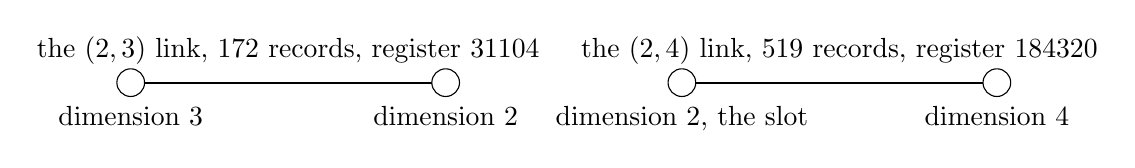
\begin{tikzpicture}[scale=1]
\draw[thick] (0,0) -- (4,0);
\filldraw[fill=white] (0,0) circle (5pt) node[below=5pt] {dimension 3};
\filldraw[fill=white] (4,0) circle (5pt) node[below=5pt] {dimension 2};
\node at (2,0) [above=3pt] {the $(2,3)$ link, 172 records, register $31104$};
\draw[thick] (7,0) -- (11,0);
\filldraw[fill=white] (7,0) circle (5pt) node[below=5pt] {dimension 2, the slot};
\filldraw[fill=white] (11,0) circle (5pt) node[below=5pt] {dimension 4};
\node at (9,0) [above=3pt] {the $(2,4)$ link, 519 records, register $184320$};
\end{tikzpicture}\caption{The two links whose dressings per unit are compared: the (2,3) link of the Ward-functional entry and the (2,4) link at the W-word pair ket with its slot at the qubit end.}\end{figure}
\end{chproof}

\section{The charged and neutral currents}\label{mod:VI-4-charged-and-neutral-currents}
\chdesig{8-4}{6-4}{VI-4-charged-and-neutral-currents}{VI-4-D538994-w-cchs}
\chinstrument{VIII}{bb1c957f1bb52ab8}
\begin{chtable}[The currents chapter]
Two results are placed at this chapter: the charged current as the hub step at every sink, an open result, and the neutral current as the Z read at the whole sinks, a theorem, each stated and derived at its own section below.
\end{chtable}
\chstanding{instrument}
\chdeps{}{}
The box is a table of the chapter arrangement; this chapter gathers two results of the weak Part, the charged current as the one move that changes a generation label, with the sink at which a second move does so named, and the neutral current as a read posed at every whole sink, with the electroweak mixing a corollary of that read.
\begin{chbridge}
What this chapter calls the hub step at a sink the literature calls the charged current carried by the W, and the two-line read at a whole sink the neutral current carried by the Z. The mixing cell of the read answers to the weak mixing angle, the nearest object. The weak interaction has two currents, the charged current, carried by the W, which changes the flavor of the fermion it acts on and couples to the left-handed fields alone, and the neutral current, carried by the Z, which conserves flavor and couples to left-handed and right-handed fields with strengths fixed by the weak mixing angle. The neutral current was observed in the heavy-liquid bubble chamber at the proton synchrotron ahead of the discovery of the bosons themselves \cite{Weinberg1967,Hasert1973}. The correspondence is by name.
\end{chbridge}
\begin{chproof}[instrument]
The table of the box in full, with its columns, the chapter, its title at the frame, its status word and the results placed at it with their standing.
\begin{center}\small
\begin{adjustbox}{max width=\linewidth}\begin{tabular}{llll}
\hline
chapter & title & status & results placed, with their standing \\
\hline
6-4 & the charged and neutral currents & filled & the charged current as the hub step at every sink, an open result; the neutral current as the Z read at the whole sinks, a theorem \\
\hline
\end{tabular}\end{adjustbox}
\end{center}
The rule that produced it. Every result is placed at one chapter by its labels and keywords, the weak results at Part VIII by the keyword rule, and a chapter reached by at least one result carries the status word filled.

The two results are derived at their own sections below. The rate of the Z read is the Born square with the cross term zero and its mixing cell the Born share, the same at every sink, and the charged current is located at every sink with the sink at which the two kinds of move part named.

\emph{Check.} The chapter table was re-cut at two engines and read the same row for row, and the two results named at this chapter stand at the index of the machine-checked package at their labels.
The rate of either current at a decay is the matter of the chapter on beta decay and of the decay chapters of Part XII.
\end{chproof}
\label{chend:VI-4-charged-and-neutral-currents}

\section{The neutral current as the Z read at the whole sinks}\label{mod:VI-4-D538865-nczr-t1}
\chinstrument{VIII}{12bb9ebd7f6bc09b}
\begin{chtheorem}[The neutral current as the Z read at the whole sinks]
The neutral current is the read of the Z at the whole sinks: the two-line read of the W word is re-posed at a (2,4) junction leg of every catalogued whole sink and is posed at all six objects, a move at every whole sink, with the rate the Born square and the cross term zero, and the electroweak mixing a corollary of the read, the Born share of the centre line equal to one minus the Born square of the W-to-Z ratio at every object and every form.
\end{chtheorem}
\chstanding{theorem}
\chdeps{}{}
The box takes the Z of the second chapter of this Part, a read along two orthogonal lines, and poses it at a junction leg of each of the six whole stable webs the letter has, it is a legitimate move at every one, it is distinct from the W read, it leaves the generation unchanged, its rate is an exact number, and the share of the rate carried by the center line is the same at every web.
\begin{chbridge}
What this chapter calls the Z read at a whole sink the literature calls the neutral-current coupling of the Z to a fermion. The Born share of the center line answers to the squared sine of the weak mixing angle and the ratio of the two rates to the ratio of the squared boson masses, the nearest objects. The neutral current couples the Z to every fermion with a vector and an axial coupling fixed by its weak isospin and its electric charge through the weak mixing angle, flavor-conserving at the tree level, and the rate of a neutral-current process is the squared amplitude of the Z exchange with the interference of the photon exchange at the same vertex \cite{Weinberg1967,Hasert1973}. The correspondence is by name.
\end{chbridge}
\begin{chproof}[finite computation]
The premises are the Z as the two-line read of chapter 6-2, an open result, the currents chapter above and the whole sinks of chapters 8-1 and 8-3, theorems and open results. The chain from the axiom to this result is seven chapters long. The procedure. The input objects are the six whole sinks, the electron sink (9 sites, 10 links, the measure 79, one hub), the muon sink (13, 15, 117, two hubs), its three tau-form sinks (15, 18, 141, 16, 19, 161, 15, 18, 146, three hubs each) and the Z body itself (the W word of measure 28). At each object the enumeration lists its (2,4) junction legs (3, 6, 9, 7, 7 and 2) and poses the two carrier lines at one of them. The test is that the two passed blocks are orthogonal at the trace form, that the sum at both lines differs from the sum at one, and that the hub count is unchanged. The aggregation is the rate, the washed square of the read, which at an orthogonal pair of lines equals the sum of the two squares with no cross term. The smallest instance is the Z body, with the word sum 28 at the count form, where both weights are 1,
\begin{equation}
S_W = 28, \qquad S_U = 28, \qquad S_Z^{2} = 784 + 784 = 1568 , \qquad \frac{S_Z^{2}}{S_W^{2}} = 2 .
\end{equation}

At the electron sink, with the whole sum 79, the same steps give the rate of the Z read against the rate of the W read,
\begin{equation}
12482 = 6241 + 6241 , \qquad \frac{S_U^{2}}{S_Z^{2}} = \frac{6241}{12482} = \frac{1}{2} = 1 - \frac{S_W^{2}}{S_Z^{2}} ,
\end{equation}
the mixing identity of the box. At the muon sink 27378 against 13689, at the three tau-form sinks 39762 against 19881, 51842 against 25921 and 42632 against 21316, the rate nonzero at 36 of 36 object-forms, the ratio 2 at the count, pair and sup-pair forms, 17 at the sup-near form, 37 at the direct-sum form and 10 at the mixed form, equal to the office of chapter 6-2 at every form, and the Born share of the center line one half, sixteen seventeenths, thirty-six thirty-sevenths and nine tenths at those forms, the same cell at every sink. The seven clauses, the lines orthogonal, the read posed at 6 of 6, distinct at 6 of 6, generation-preserving at 6 of 6, the rate a cell at 6 of 6, the mixing identity at 6 of 6 and the sinks re-met at 6 of 6, are all met, and the first object at which a clause parts is none.

\emph{Check.} What would have broken the result, the center line struck at every form moves the Z read onto the W read, the ratio to 1 and the mixing cell to 0, so the read is distinct at 0 of 6. The amplitude sum in place of the orthogonal sum moves the rate to the square with its cross term, the ratio to 4 at the count form, and the mixing identity parts at 0 of 36. The literature text struck moves the gate to unmet. The result was reproduced by an independent route, two engines at every capture byte for byte, its four counter-tests at their pinned letters and its sixteen controls the same at both routes.
The mixing cells and the rate ratios are compared with experiment at the comparison table of this compendium.
\chcert{36}
\end{chproof}
\label{chend:VI-4-D538865-nczr-t1}

\section{The charged current as the hub step at every sink}\label{mod:VI-4-D538994-w-cchs}
\chinstrument{VIII}{5c28ce01ab677ccb}
\begin{chwall}[The charged current as the hub step at every sink]
The charged current is the hub step at every catalogued sink: the hub step is one of two kinds of move that change the generation label at the sinks, the hub-forming move of the pair-production row the other at twelve of the thirteen sinks and the hub step alone at the roster forms, and the rate of the step is exact at every sink. On the one face the thirteen sinks are located and the rate of the hub step is an exact cell at every one; on the other face the generation label is changed by one kind of move at one sink alone, the catalogued tau, and the parting is named at the electron sink, where the hub step and the hub-forming move both change the label, with both cells.
\end{chwall}
\chstanding{open result, built and not closed}
\chdeps{}{}
The box asks whether the weak interaction of this compendium, the hub step, is the only move that changes a generation at a stable web. It is not, a second move does so at twelve of thirteen webs, and the open result stands at the first of them, the electron, with the rate of each move printed.
\begin{chbridge}
What this chapter calls the hub step at a sink the literature calls the charged-current transition of a fermion, and its rate cell the squared amplitude of the transition, the nearest object. The hub-forming move of the pair-production row has no name in the literature. The charged current of the weak interaction changes the flavor of the fermion it acts on, a charged lepton to its neutral partner or an up-type quark to a down-type quark of any generation with the amplitude of the mixing block, couples to the left-handed fields alone and is carried by the W. Every weak decay of a charged lepton or of a quark proceeds through it at the tree level \cite{Fermi1934,Weinberg1967,Cabibbo1963}. The correspondence is by name.
\end{chbridge}
\begin{chproof}[finite computation]
The premises are the moves in one table of chapter 1-4, a definition, the hub step as the weak interaction of chapter 6-1, an open result, and the currents chapter above. The chain from the axiom to this result is seven chapters long. The procedure. The input objects are the thirteen sinks located at the primary set of the decay graph, the electron sink (9 sites, 10 links, the measure 79, one hub, the dressing 3, the first power 201), the muon sink (13, 15, 117, two hubs, 9, 963), the tau (17, 20, 155, three hubs, 27, 3969), the proton sink (10, 12, 101, one hub, 27, 2727), its neutron twin (13, 16, 133, two hubs, 81, 10773), two further proton sinks and six docked quark bodies. The enumeration lists every edge leaving a sink and types it by the move table, the hub step and its reverse at plus and minus one hub, the hub-forming move and its reverse at plus and minus one, the attachments and the joins at zero, the typing equal to the recorded change at 182 of 182 edges. The test is whether the edge changes the hub count, the generation label. The aggregation is the rate by the rate law, the readout of an edge the measure the move adds or removes multiplied by the dressing of the sink, the washed square the sum of the squared readouts, and the cell the washed square over the first power squared. The smallest instance is the docked up quark, three sites, two links, the measure 12, no hub, the dressing 1 and the first power 6, four generation-changing edges and the cell
\begin{equation}
\frac{5792}{36} = \frac{1448}{9} .
\end{equation}

At the electron sink the hub step acts forward at sixteen edges with the readouts 93 to 120 at the dressing 3, and the rate cell of the charged current there is
\begin{equation}
\frac{176067}{201^{2}} = \frac{176067}{40401} = \frac{19563}{4489} ,
\end{equation}
with the inverse step at five edges at the cell $7310/4489$. The hub-forming move of the pair-production row acts forward at one edge there at the cell
\begin{equation}
\frac{676}{4489} ,
\end{equation}
so two kinds of move change the generation label at the electron, the parting of the box. The forward cells at the thirteen sinks are $19563/4489$, $34958/11449$, $2987/2401$, $11002/10201$, $23467/17689$, $11770/3969$, $26051/5776$, $1448/9$, $4170/529$, $1099/100$, $417/160$, $1474/361$ and $4271/1682$, the muon and tau cells equal to the rate-law entry. At the cataloged tau alone the hub step is the one kind, 29 edges, 22 forward and 7 inverse, its one triangle edge a join at two qubits at zero change.

\emph{Check.} At the reading that admits only targets the construction has recorded, the hub step is the one kind at 9 of 13 sinks and the first parting moves to the proton sink, which reaches no recorded web by a generation-changing edge. At the reading over bodies alone the same. The result was reproduced by an independent route, two engines at every capture byte for byte, its five counter-tests at their pinned letters and its controls the same at both routes but one, a cross-route comparison at one key beyond the native integer range of one route, exact at the other and equal at the re-meet.
The second kind of move, the hub-forming move of the pair-production row, changes the generation label beside the hub step at twelve of the thirteen sinks.
\chcert{182}
\end{chproof}
\label{chend:VI-4-D538994-w-cchs}

\section{The Fermi constant and the muon decay}\label{mod:VI-5-fermi-constant-and-the-muon-decay}
\chdesig{8-5}{6-5}{VI-5-fermi-constant-and-the-muon-decay}{VI-5-D538919-w-fcwo}
\chinstrument{VIII}{3f466d2f4dcd65f9}
\begin{chtable}[The Fermi-constant chapter]
One result is placed at this chapter: the Fermi constant as the office of the W word at low transfer, an open result named at its first parting, stated and derived at its own section below; the rate of the hub step over the fifth power of the first power, the mass unit of the construction, is an exact cell at each of the three bodies, the muon, the roster tau and the beta arm, read against the W office 784 over 4489.
\end{chtable}
\chstanding{instrument}
\chdeps{}{}
The box is a table of the chapter arrangement; this chapter gathers the one result of the weak Part on the Fermi constant, whose three cells are exact and whose universality across the three bodies is what the result leaves open, the tau being the first body to part.
\begin{chbridge}
What this chapter calls the office of the W word at low transfer the literature calls the Fermi constant, and the rate of the hub step over the fifth power of the first power the muon decay rate over the fifth power of the muon mass. The equality of the cell across the three bodies answers to the universality of the weak coupling, the nearest object. In the four-fermion theory of the weak interaction the muon decays through a contact interaction whose strength is the Fermi constant, the decay rate proportional to the fifth power of the muon mass with the Fermi constant squared as the coefficient, and the same constant governs the beta decay of the neutron and the decay of the tau. In the electroweak theory the Fermi constant is the low-transfer limit of the W exchange, the square of the gauge coupling over the square of the W mass up to a numerical factor \cite{Fermi1934,Michel1950,Weinberg1967}. The correspondence is by name.
\end{chbridge}
\begin{chproof}[instrument]
The table of the box in full, with its columns, the chapter, its title at the frame, its status word and the result placed at it with its standing.
\begin{center}\small
\begin{adjustbox}{max width=\linewidth}\begin{tabular}{llll}
\hline
chapter & title & status & result placed, with its standing \\
\hline
6-5 & the Fermi constant and the muon decay & filled & the Fermi constant as the W word office at low transfer, an open result named at its first parting \\
\hline
\end{tabular}\end{adjustbox}
\end{center}
The rule that produced it. Every result is placed at one chapter by its labels and keywords, the weak results at Part VIII by the keyword rule, and a chapter reached by at least one result carries the status word filled.

The result is derived at its own section below. The decay of the muon as a cell of the decay table stands at the first chapter of Part XII.

\emph{Check.} The chapter table was re-cut at two engines and read the same row for row, and the result named at this chapter stands at the index of the machine-checked package at its label.
One cell of the Fermi constant across the three bodies is what stays open. The lifetime of the muon is compared with experiment in the comparison table.
\end{chproof}
\label{chend:VI-5-fermi-constant-and-the-muon-decay}

\section{The Fermi constant as the W word office at low transfer}\label{mod:VI-5-D538919-w-fcwo}
\chinstrument{VIII}{6c99388999923345}
\begin{chwall}[The Fermi constant as the W word office at low transfer]
The Fermi constant is the office of the W word at low transfer: the rate of the hub step over the fifth power of the first power is an exact cell at each of the three bodies, the muon, the roster tau and the beta arm, against the W office 784 over 4489. On the one face the three cells are defined and exact; on the other face they are equal across the bodies at no reading of the grid, zero of its twelve pairs, the first body to part the tau, with both cells named.
\end{chwall}
\chstanding{open result, built and not closed}
\chdeps{}{}
The box forms, at each of three decaying webs, the number the literature would form from a decay rate and a mass, the rate divided by the fifth power of the mass unit, and asks whether the three numbers agree, as universality would demand. They are exact, and they do not agree.
\begin{chbridge}
What this chapter calls the office of the W word the literature calls the Fermi constant, the hub-step rate the decay rate, the first power the mass of the body and the beta arm the neutron. The equality of the cell across the bodies answers to the universality of the weak coupling, the nearest object. The Fermi constant is the strength of the four-fermion contact interaction of the weak decays, in the electroweak theory the low-transfer limit of the W exchange proportional to the square of the gauge coupling over the square of the W mass, and the same constant governs the muon decay, the tau decays and the beta decay of the neutron, the universality of the weak coupling across the lepton families tested at the ratio of the muon and tau rates with the fifth power of the masses \cite{Fermi1934,Michel1950,Weinberg1967}. The correspondence is by name.
\end{chbridge}
\begin{chproof}[census]
The premises are the Fermi-constant chapter above, the mass unit and the first power of chapter 8-1, a theorem, and the W and the Z of chapter 6-2, an open result, the chain from the axiom seven chapters long. The set counted is the grid of readings, three readings of the rate axis by two spellings of the first power with twelve ordered pairs of bodies at each, and the property tested is the equality of the cell at two bodies. The exact part first. From the first powers at the hub spelling, the rank multiplied by the dressing,
\begin{equation}
963 = 107 \cdot 9, \qquad 3969 = 147 \cdot 27, \qquad 10773 = 133 \cdot 81 ,
\end{equation}
at the muon, the tau and the neutron of the beta arm, by the fifth power, we obtain $963^{5}$, $3969^{5}$ and $10773^{5}$. From the hub-step rates, the washed forward rates $34958/11449$ at the muon over 29 edges and $2987/2401$ at the tau over 22 edges and the arm cell $36/17689$ at the neutron, by division, we obtain the three cells of the box,
\begin{equation}
\frac{34958}{11449 \cdot 963^{5}}, \qquad \frac{2987}{2401 \cdot 3969^{5}}, \qquad \frac{36}{17689 \cdot 10773^{5}} ,
\end{equation}
From the office row, by the square of the first power of the W word over the unit, the W office at the dock face and at the hub face is
\begin{equation}
\Bigl(\frac{28}{67}\Bigr)^{2} = \frac{784}{4489}, \qquad \Bigl(\frac{28}{201}\Bigr)^{2} = \frac{784}{40401} ,
\end{equation}
and the quotients of the three cells by the dock-face office stand as exact rationals.

The census part. Over the twelve pairs of the grid the cells are defined at 6 of 12 (the three bodies at the two spellings) and equal at 0 of 12. The first parting in the order of the bodies is the tau, its cell against the muon cell, the arm parting beside, the ratio of the tau cell to the muon cell an exact rational of eighteen digits over twenty-two. The tau of the box is the roster tau, no tau-form sink of the saturation being the roster tau or carrying a recorded rate cell. The smallest case is the muon alone, its cells at the hub and dock spellings differing by the fifth power of the dressing 9, the fifth power of 963 against that of 107.

\emph{Check.} The comparison rests on no reading of the W office, which divides every cell alike, and the control on the link genres, mis-posed at one string spelling, read the same at its adopted spelling at all 1691 links. The result was reproduced by an independent route, two engines at every capture byte for byte, its five counter-tests and sixteen controls at their pinned letters.
\chcert{12}
\end{chproof}
\label{chend:VI-5-D538919-w-fcwo}

\section{The electroweak table}\label{mod:VI-9-electroweak-table}
\chinstrument{VIII}{a360e896860a648a}
\begin{chtable}[The electroweak table]
This chapter is reserved for the electroweak table, the one table that gathers the exact cells of this Part, by our arrangement of the weak Part; no result is placed at it, its status awaiting its result, and the cells it will gather stand at their own chapters.
\end{chtable}
\chstanding{instrument}
\chdeps{}{}
The box is a table of the chapter arrangement; this chapter exists as the place where the weak angle, the Fermi constant, the W and the Z, the Higgs and carrier offices, the quark mixing block and the boson widths would be gathered into one table.
\begin{chbridge}
What this chapter would gather the literature calls the electroweak parameters, the two gauge couplings, the weak mixing angle, the masses of the W, the Z and the Higgs, the Fermi constant and the widths of the bosons. The electroweak sector of the Standard Model is summarized at one table of its parameters, related among themselves at the tree level by the relations of the theory and confronted together at a global fit of the precision data \cite{Glashow1961,Weinberg1967,Salam1968}. The correspondence is by name.
\end{chbridge}
\begin{chproof}[instrument]
The table of the box in full, with its columns, the chapter, its title at the frame, the decision of ours that reserved it, its status word and the cells it will gather.
\begin{center}\small
\begin{adjustbox}{max width=\linewidth}\begin{tabular}{lllll}
\hline
chapter & title & reserved by & status & cells to gather \\
\hline
6-9 & the electroweak table & our arrangement of the weak Part & awaiting its result & the weak angle; the Fermi constant; the W and the Z; the Higgs and carrier offices; the quark mixing block; the boson widths \\
\hline
\end{tabular}\end{adjustbox}
\end{center}
The rule that produced it. Every result is placed at one chapter by its labels and keywords, and a chapter that the frame names by a decision of ours and that no result reaches carries the status awaiting its result.

The table itself is a composition of the cells of this Part at the comparison table of this compendium, every cell compared with experiment there.

\emph{Check.} The chapter table and the empty-chapters table were re-cut at two engines and read the same row for row. The status word of this chapter was carried unchanged.
The electroweak table as one composition of the cells of this Part is to be written once its result is placed here.
\end{chproof}
\label{chend:VI-9-electroweak-table}

\section{The electroweak breaking as the stabilizer of the vacuum register}\label{mod:VI-9-D543021-vcst-t1}
\chinstrument{VIII}{853c39e74af2ef50}
\begin{chconditional}[The electroweak breaking as the stabilizer of the vacuum register]
This theorem is conditional on the entries its provenance names at the grades their grade lines print, the open results among them read at their own grades. The electroweak breaking as the vacuum stabilizer: the stabilizer of the (4,4) vacuum register, the pair ket of the hub link at its common support four with its register 6561, the clauses whole 81 to the order exponent two as the curvature-coefficient, quartic, Higgs-office and Higgs-and-carrier entries carry it, inside the algebra spanned by the (2,3) center $3,3,-2,-2,-2$ and the (2,4) center $2,2,-1,-1,-1,-1$ is one line and its direction is the (2,3) center alone: at the reading adopted the (2,4) center acts at the two ququart ends of the hub link as the scalar minus two and is broken at the vacuum, the (2,3) center carries no block at the ququart and annihilates the vacuum register, the unbroken direction one, zero equal to the (2,3) center at both engines and both runs; the readings beside, the nested levels and the pair scalars, at which the direction parts, printed at the grid beside the result; the breaking at the ququart and the (2,3) center the survivor.
The first face, the unbroken direction the (2,3) center, the breaking at the ququart and the (2,3) center the survivor, reads yes, the stabilizer of dimension one at the direction one, zero; the second face, another direction named, reads no at the reading adopted and is met at the readings beside, the nested level at the clauses support at the direction one, minus two and the pair scalar at one, minus one, printed beside the result.
\end{chconditional}
\chstanding{a conditional theorem}
\chdeps{}{}
The vacuum of the model is the pair ket of the (4,4) link at the hub, and the two centers available at the hub are the central lines of the identification algebras at the (2,3) and the (2,4) genres, which together span an abelian algebra of dimension two. A center acts on the vacuum register through its block at an end of the same dimension. The (2,4) center has a ququart block and reads minus two on the vacuum, so it is broken there; the (2,3) center has no ququart block and reads zero, so it leaves the vacuum invariant. The subalgebra that stabilizes the vacuum is therefore the one line of the (2,3) center, which is the direction the stabilizer and photon entries of the fine-structure chapter name as the acting charge of the letter.
\begin{chbridge}In the electroweak theory the Higgs vacuum expectation value breaks the product of the weak isospin and hypercharge groups to the electromagnetic subgroup, the one combination of the two generators that annihilates the vacuum, and the photon is its gauge boson \cite{Weinberg1967,Peskin1995}. The literature names the vacuum register as nearest a vacuum expectation value, the two centers as nearest the hypercharge and the third weak isospin generators, the stabilizer as the unbroken subgroup, exact as a group-theoretic notion, and the electroweak breaking by name. The correspondence is by name.\end{chbridge}
\begin{chproof}[finite computation with its exact part]
The premises of this derivation are the axiom and the six definitions of chapter~\ref{mod:FRAMEWORK}, the electroweak table of the present chapter, an instrument, the link and its six genres of chapter~\ref{mod:I-2-link-and-its-six-genres}, a theorem, the stabilizer of the pair ket and the photon of chapter~\ref{mod:V-1-fine-structure-constant-at-the-one-link}, an open result and a theorem, and the Higgs quartic of chapter~\ref{mod:VI-10-higgs-the-closed-hub-read-its-rows-its-mass-and-its-exponent}, a theorem. The chain of premises runs back to the axiom through those chapters, and the longest such chain in this compendium is twelve chapters long.
\textit{The object.} The vacuum register is the pair ket of the (4,4) genre at its common support four on the tensor register of dimension sixteen, the sixteen coordinates one at the four matched directions and zero elsewhere, with the unit 16, the whole 256 and the cut 225, and its register 6561, the (3,3) whole 81 to the order exponent two, located equal at the four parent entries. The figure draws the hub link with the blocks of the two centers.
\textit{The procedure.} Re-derive the identification algebra at every genre from its basis by kind and label and close the brackets, 49, 144, 361, 289, 576 and 961 at the six genres; take the center at each, one line equal to the traceless element; take the (2,3) and (2,4) centers at their primitive diagonals and span an algebra of dimension two. Let a center act on the vacuum register through its block at an end of the same dimension, the reading adopted, and compute the null space of the two action vectors, the real and imaginary parts stacked; its dimension and direction in the basis of the two centers are the stabilizer.
\textit{The smallest instance.} The (2,4) center has the ququart block $\mathrm{diag}(-1,-1,-1,-1)$ and acts at both ends of the hub link, while the (2,3) center has blocks at the dimensions two and three alone and none at the ququart, so on the vacuum register
\begin{equation} C_{24}\,\lvert\Phi_{44}\rangle = \big((-1) + (-1)\big)\lvert\Phi_{44}\rangle = -2\,\lvert\Phi_{44}\rangle, \qquad C_{23}\,\lvert\Phi_{44}\rangle = 0 , \end{equation}
and an element $a\,C_{23} + b\,C_{24}$ annihilates the vacuum if and only if $-2b = 0$, so the stabilizer is the line $(a, b) = (1, 0)$, the (2,3) center alone, of dimension one. At the readings beside, the nested level at the clauses support gives the direction $(1,-2)$ and the pair scalar $(1,-1)$, each printed at the grid beside the result; at the end mask reading the Higgs word alone the whole span survives.
\textit{The check.} The counter-tests alter the construction singly and read what moves. Striking the (2,4) center widens the stabilizer to the whole span of dimension two. Reading the (3,3) center in place of the (2,4), with blocks at the dimension three alone, leaves the whole span. Shifting the register to the (3,4) genre reads the (2,3) center at the qutrit end as minus two and the (2,4) center at the ququart end as minus one, the direction $(1,-2)$ and the second face. Striking the text unmeets the gate. Reading the stabilizer at the (2,3) pair ket in place of the vacuum register gives the direction $(2,-1)$. Each alteration moves the cells it names, five of five. The result was reproduced by an independent route, two engines built apart, the key-value and fraction route against the second route, equal at every cell, with the fourteen controls the same.
\chcert{6}
\begin{figure}[h]\centering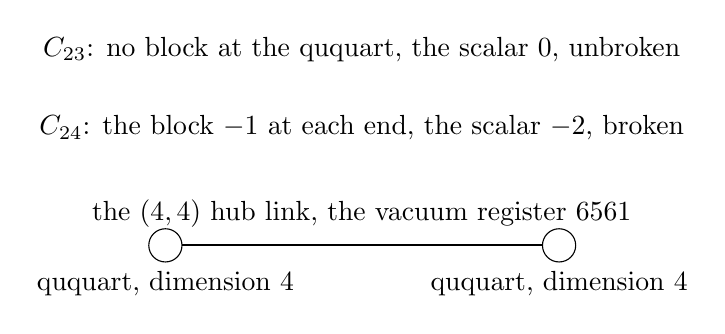
\begin{tikzpicture}[scale=1]
\draw[thick] (0,0) -- (5,0);
\filldraw[fill=white] (0,0) circle (6pt) node[below=6pt] {ququart, dimension 4};
\filldraw[fill=white] (5,0) circle (6pt) node[below=6pt] {ququart, dimension 4};
\node at (2,0) [above=3pt, xshift=14pt] {the $(4,4)$ hub link, the vacuum register $6561$};
\node at (2,1) [above=6pt, xshift=14pt] {$C_{24}$: the block $-1$ at each end, the scalar $-2$, broken};
\node at (2,2) [above=6pt, xshift=14pt] {$C_{23}$: no block at the ququart, the scalar $0$, unbroken};
\end{tikzpicture}\caption{The hub link whose pair ket is the vacuum register, with the action of the (2,4) center and of the (2,3) center at its two ququart ends.}\end{figure}
\end{chproof}

\section{Chiral breaking and the theta angle}\label{mod:VII-8-chiral-breaking-and-the-theta-angle}
\chdesig{9-8}{7-8}{VII-8-chiral-breaking-and-the-theta-angle}{VII-8-chiral-breaking-and-the-theta-angle}
\chinstrument{IX}{a18c245381697a58}
\begin{chtable}[The chiral-breaking chapter]
This chapter is reserved for chiral breaking and the theta angle by two decisions of ours, with no result placed at it, its status awaiting its result; the corollary theorem of the hadron spectrum names chiral symmetry at the pion entry among its six gated entries, the pion resting on the least two-core pairing of the pairing move with the order lightest supplied by no established clause, and the theta angle awaits its result.
\end{chtable}
\chstanding{instrument}
\chdeps{}{}
The box is a table of the chapter arrangement; this chapter exists as the place reserved for two results the construction has still to supply.
\begin{chbridge}
What this chapter would hold the literature calls the spontaneous breaking of chiral symmetry and the theta angle of the gauge vacuum. The least two-core pairing of the pairing move answers to the pion by name at the corollary theorem. The chiral symmetry of the light-quark sector of quantum chromodynamics is broken spontaneously by the quark condensate, the pions the pseudo-Goldstone bosons of that breaking with masses that vanish as the light-quark masses vanish \cite{NambuJonaLasinio1961,Goldstone1961}. The gauge vacuum admits a term proportional to a theta angle that violates the combined charge and parity symmetry, and the smallness of that angle is the strong CP problem, addressed by the axion proposal \cite{tHooft1976,PecceiQuinn1977}. The correspondence is by name.
\end{chbridge}
\begin{chproof}[instrument]
The table of the box in full, with its columns, the chapter at the frame cited (its number at that frame, ahead of the weak Part inserted since), its title, the decisions of ours that reserved it, its status word and the entries naming its subject since.
\begin{center}\small
\begin{adjustbox}{max width=\linewidth}\begin{tabular}{lllll}
\hline
chapter at the frame cited & title & reserved by & status & entries naming its subject \\
\hline
the eighth chapter of the hadron Part & chiral breaking and the theta angle & two decisions of ours & awaiting its result & the corollary theorem of the hadron spectrum at its pion entry \\
\hline
\end{tabular}\end{adjustbox}
\end{center}
The rule that produced it. Every result is placed at one chapter by its labels and keywords, and a chapter that the frame names by a decision of ours and that no result reaches carries the status awaiting its result. The chapter count of the frame was settled with four results added as chapters.

The theta angle as the junction holonomy stands placed at this chapter by the index of the machine-checked package, and its text is still to be written here.

\emph{Check.} The chapter table and the empty-chapters table were re-cut at two engines and read the same row for row. The status word of this chapter was carried unchanged.
Chiral breaking at the pion entry of the corollary theorem and the theta angle are to be written once their results are placed here.
\end{chproof}
\label{chend:VII-8-chiral-breaking-and-the-theta-angle}

\section{The mesons and the nucleon at the cap}\label{mod:VII-9-mesons-and-the-nucleon-at-the-cap}
\chinstrument{IX}{0edadc6636395c7d}
\begin{chtable}[The cap chapter]
Six results are placed at this chapter: the counterfactual hub at the three-quark web, the proton control at the bond, the sector identity at the genre, the mass ratio at the hydrogen bond, the far-end rule as the end-set selector at every dock link and the pion at the cap, two theorems, three open results and one instrument among them, each at its own standing, the chapter awaiting its writing.
\end{chtable}
\chstanding{instrument}
\chdeps{}{}
The box is a table of the chapter arrangement; six results of the construction on the mesons and the nucleon at the cap of a genre are placed here by their labels, and the chapter that states and derives them is still to be written.
\begin{chbridge}
What this chapter would hold the literature calls the pion, the nucleon and the hydrogen bond. The cap of a genre answers to the dimension of a record space, the nearest object. The pion, the nucleon and the hydrogen bond are the standard objects of the subject of this chapter \cite{Yukawa1935}. The chapter awaits its writing. The correspondence is by name.
\end{chbridge}
\begin{chproof}[instrument]
The table of the box in full, with its columns, the chapter at the frame cited (its number at that frame, ahead of the weak Part inserted since), its title, its status word and the results placed at it.
\begin{center}\small
\begin{adjustbox}{max width=\linewidth}\begin{tabular}{llll}
\hline
chapter at the frame cited & title & status & results placed \\
\hline
the ninth chapter of the hadron Part & the mesons and the nucleon at the cap & filled & the counterfactual hub at the three-quark web; the proton control at the bond; the sector identity at the genre; the mass ratio at the hydrogen bond; the far-end rule as the end-set selector at every dock link; the pion at the cap \\
\hline
\end{tabular}\end{adjustbox}
\end{center}
The rule that produced it. Every result is placed at one chapter by its labels and keywords, the six results here by our decisions on the cap, and a chapter reached by at least one result carries the status word filled.

The six results stand each at its own standing at the index of the machine-checked package.

\emph{Check.} The chapter table was re-cut at two engines and read the same row for row. The six labels placed at this chapter stand at the index of the machine-checked package.
The chapter itself awaits its writing, every result placed here standing at its own standing.
\end{chproof}
\label{chend:VII-9-mesons-and-the-nucleon-at-the-cap}

\section{Alpha decay}\label{mod:IX-5-alpha-decay}
\chdesig{12-5}{9-5}{IX-5-alpha-decay}{IX-5-alpha-decay}
\chinstrument{XII}{93b5c22aaddd62ae}
\begin{chtable}[Alpha decay]
The chapter awaits the derivation of alpha decay as a forward edge of the move graph at the joined seeded webs. The chapter of a prior arrangement of this compendium that carried beta decay, alpha decay and the boson widths together stands retitled into this one, its results placed where the arrangement names them.
\end{chtable}
\chstanding{instrument}
\chdeps{}{}
The chapter of a prior arrangement of this compendium that carried beta decay, alpha decay and the boson widths together stands retitled into this one, its results placed where the arrangement names them, and the chapter waits on alpha decay as a forward edge of the move graph at the joined seeded webs. The boson widths and the beta release of the prior arrangement stand at the chapter of beta decay and the widths, the binding of the alpha as the pairing records at the next chapter, and the alpha lines of the decay board, owed with the nuclear half-lives.
\begin{chbridge}
Alpha decay is the escape of a preformed alpha particle from the nucleus by quantum tunneling through the Coulomb barrier of the daughter, the decay rate set by the barrier penetration factor, exponentially sensitive to the decay energy, so that the logarithm of the half-life is a linear function of the inverse square root of that energy across the alpha emitters \cite{Gamow1928,Gurney1928,Geiger1911}. The alpha is the joined seeded web of two protons and two neutrons by name, the forward edge is a decay channel by name, the rate is nearest the washed square of the read per tick, and the pairing record is nearest a record of two bodies at a shared site. The correspondence is by name.
\end{chbridge}
\begin{chproof}[instrument table]
The table of this chapter is the placement of the arrangement adopted. The chapter awaits the derivation of alpha decay as a forward edge of the move graph at the joined seeded webs, and the rule that produced the placement names this chapter as awaiting its derivation and places the results of the prior arrangement at the chapters of beta decay and the widths, of the binding of the alpha, and of the decay board.
\end{chproof}

\section{Fission, fusion and stellar bounds}\label{mod:IX-8-fission-fusion-and-stellar-bounds}
\chinstrument{XII}{f4405bdc5ceca4a0}
\begin{chtable}[Fission, fusion and stellar bounds]
The chapter awaits the derivations of fission, fusion and the stellar bounds.
\end{chtable}
\chstanding{instrument}
\chdeps{}{}
The chapter waits on fission and fusion and the stellar bounds. The process census of the first chapter of this Part names the binding and the fusion among its three spelled kinds at the pairing move across webs and the two-star sink, the derived words at fusion so far. The alpha cluster as what the cut releases stands at its open question.
\begin{chbridge}
In the standard account fission is the splitting of a heavy nucleus into two fragments with a release of energy read off the mass formula, the liquid-drop picture of the deformed nucleus and its barrier \cite{BohrWheeler1939}. Fusion is the joining of light nuclei into heavier ones, the chains of reactions that power the stars \cite{Bethe1939}. The stellar bounds are the limiting masses of the stars and their remnants, the balance of pressure and gravity at the degenerate configurations \cite{Chandrasekhar1931}. The pairing move is nearest an entanglement swap creating a pair between two ends, the star is nearest a star graph, the cut is nearest the removal of an edge, and the sink is nearest a fixed point of the dynamics. The correspondence is by name.
\end{chbridge}
\begin{chproof}[instrument table]
The table of this chapter is the placement of the arrangement adopted. The chapter awaits the derivations of fission, fusion and the stellar bounds, and the rule that produced the placement names this chapter as awaiting its derivations.
\end{chproof}

\section{The equilibrium theorem}\label{mod:XI-6-equilibrium-theorem}
\chdesig{13-6}{11-6}{XI-6-equilibrium-theorem}{XI-6-equilibrium-theorem}
\chinstrument{XIII}{d627a47c7706199d}
\begin{chtable}[The equilibrium theorem, awaited]
This chapter is counted as awaiting its derivation, the equilibrium theorem, with no result placed at it.
\end{chtable}
\chstanding{instrument}
\chdeps{}{}
What the chapter waits on is an equilibrium theorem still to be stated. The thermal state stands as a definition at every cap with the Gibbs form an output of it at no finite network, parting at the second order through a joined network with a bath body, and the zeroth and third laws stand as exact objects among the cap readings, so the chapter will be written when that derivation arrives.
\begin{chbridge}
The literature calls the cap a terminal site (nearest), the joined web the composition of two networks along shared sites (nearest), the washed marginal a reduced density matrix with the twirl applied (exact), and the object awaited the approach of an isolated system to thermal equilibrium, the state at which the entropy is at its maximum under the constraints with the temperature as its label under the zeroth law \cite{Callen1985}, the H-theorem its kinetic form with $H$ decreasing to the Maxwell distribution \cite{Boltzmann1872}. The correspondence is by name. The construction supplies a fixed point at a cap and readings at the joined networks carrying the names at Sections~\ref{mod:XI-2-thermal-state} and \ref{mod:XI-3-ensembles-as-cap-readings}, and the equilibrium theorem is named by correspondence.
\end{chbridge}
\begin{chproof}[instrument]
The premises are the Axiom and the six definitions of Section~\ref{mod:FRAMEWORK} (definitions), the thermal state of Section~\ref{mod:XI-2-thermal-state} (open results) and the cap readings of Section~\ref{mod:XI-3-ensembles-as-cap-readings} (a theorem). The chapter uses nothing of them beyond their statements, and the chain from the axiom to this chapter is seven chapters deep.
The table is the placement of this chapter in the arrangement of the chapters. The rule that produced it places every established result at one chapter by its reading and marks a chapter at which no result is placed as awaiting its derivation. The one column lists what the chapter reads beside and the standing of each.
\begin{center}
\begin{adjustbox}{max width=\linewidth}\begin{tabular}{ll}
\hline
what the chapter reads beside & standing \\
\hline
the thermal state as the twirl fixed point at a cap & an open result, the Gibbs form an output at no finite network \\
the thermal state through the joined web with a bath body & an open result, the marginal parting at the second order \\
the ensembles as cap readings at the joined web & a theorem, the zeroth and third laws exact objects \\
the equilibrium theorem & no result, the derivation awaited \\
\hline
\end{tabular}\end{adjustbox}
\end{center}
The check is that the three rows read beside stand at their own chapters with their counts unmoved here.
The placement was reproduced by an independent route, the two engines agreeing at every chapter of the frame.
\end{chproof}

\section{The Chern number}\label{mod:XII-4-chern-number}
\chdesig{14-4}{12-4}{XII-4-chern-number}{XII-4-D538575-flxf-t1}
\chinstrument{XIV}{f4255061730dc5dc}
\begin{chtable}[The Chern number, awaited]
This chapter is counted as awaiting its derivation; two results of that derivation are read here as they stand.
\end{chtable}
\chstanding{instrument}
\chdeps{}{}
The Chern results are to be anchored at this chapter at a later arrangement of the chapters. The section that follows adds the flux clause at the faces.
\begin{chtheorem}[The winding of the wash holonomy around one period]
At every periodic stable configuration the winding of the wash holonomy around one period, the holonomy a map on the register letters, is an exact integer, 12 twenty-fourths of a turn at every one of the 28 deciding docks, the holonomy the sign of the letter XZ on the four register letters at every odd period, invariant at every sample of the group moves and the re-matchings at 28 of 28, with the readings at the period and at the first dock agreeing and the mean reading parting.
\end{chtheorem}
\chstanding{theorem}
\chdeps{}{}
\begin{chtheorem}[The winding around the full cycle of a joined periodic network]
The winding of the wash holonomy around the full cycle of every joined periodic network, lifted per loop, equals half the count of its parity-odd stable configurations at 175 of 175 networks, the nonzero integer reached at 133 networks beyond one sink, the quantum Hall integer a name beside; the holonomy composed from the four register letters along the whole walk equals the per-loop lift at 700 of 700 cycles, its determinant inside the qubit group, so the corollary stands narrower than the hypothesis of its kind and holds.
\end{chtheorem}
\chstanding{theorem}
\chdeps{}{}
The first result is conditional on the results of its own statement, the periodic sink and the charged periodic sink among them, and the second is a corollary of the first; both are read at their own chapters.
\begin{chwall}[The flux quantization premise re-posed]
The flux quantization premise re-posed stands at this chapter as an open result read at its grade.
\end{chwall}
\chstanding{open result}
\chdeps{}{}
\begin{chbridge}
The literature calls the wash the twirl (exact), the holonomy the parallel transport around a closed path (nearest), the register letters the generalized Pauli operators (nearest), and the objects named the first Chern number of a band over the Brillouin zone, the integer of the Hall conductance in units of $e^{2}/h$ \cite{Thouless1982,Klitzing1980}, and the Berry phase as the holonomy of the band bundle \cite{Berry1984}. The correspondence is by name at the Chern number and the Berry phase as theorems of the literature. The construction supplies a winding of the wash holonomy around a period carrying the names, and the quantization of the Hall conductance is named by correspondence. The correspondence is by name at the Hall conductance and the charge, the charged class standing at Parts V and VIII. The correspondence is by name at the standard quantum objects and the geometry. The construction supplies the states and projections it uses at Section~\ref{mod:FRAMEWORK}, the ladders carrying the geometric names standing at Parts VI, X and XII.
\end{chbridge}
\begin{chproof}[instrument]
The premises are the Axiom and the six definitions of Section~\ref{mod:FRAMEWORK} (definitions), the saturation of Section~\ref{mod:I-5-saturation-in-one-figure-seeds-waves-termination-sinks} and the read at a register of Section~\ref{mod:I-6-read-at-a-register-the-probe-and-the-measurement} (theorems), the lattice of Section~\ref{mod:XII-1-lattice-as-the-periodic-sink} and the chain of pairs of Section~\ref{mod:XII-3-chain-of-pairs-and-the-charged-periodic-sink} (theorems). The chapter uses nothing of them beyond their statements, and the chain from the axiom to this chapter is eleven chapters deep.
The table is the placement of this chapter in the arrangement of the chapters. The rule that produced it places every established result at one chapter by its reading and marks a chapter at which no result is placed as awaiting its derivation. The one column lists what the chapter reads beside and the standing of each.
\begin{center}
\begin{adjustbox}{max width=\linewidth}\begin{tabular}{ll}
\hline
what the chapter reads beside & standing \\
\hline
the winding of the wash holonomy around one period & a theorem, conditional on the periodic and the charged periodic sink \\
the winding around the full cycle of a joined periodic network & a theorem, a corollary of the first \\
the flux quantization premise re-posed & an open result, read at its own statement \\
the flux clause re-posed at the face & a theorem, the section that follows \\
the Chern number & no result anchored, the derivation awaited \\
\hline
\end{tabular}\end{adjustbox}
\end{center}
The check is that the results read beside stand at their own chapters with their counts unmoved here.
The placement was reproduced by an independent route, the two engines agreeing at every chapter of the frame.
\end{chproof}

\section{The flux clause re-posed at the face}\label{mod:XII-4-D538575-flxf-t1}
\chinstrument{XIV}{a8704c2a8e2f753b}
\begin{chtheorem}[The flux clause re-posed at the face]
The flux integer per face is the fan sum of that face at every two-path network: at every one of the 45739 defined two-path networks of the base result, read as faces with the enclosed set decomposed into its fan loops (89607 fan loops), the flux integer per face, the wash integer of the base result, equals the sum of the lifts over 24 of its fan loops cell for cell at 45739 of 45739, and the Chern integer of the periodic sink is the same object at the periodic face (the winding at the period docks 28 of 28). The other readings are recorded beside the result: the whole loop with no decomposition equals the fan sum at 12874 of 45739, and the flux clause per link of the flux result at 34215 of 45739, each with its first parting named at the inserted site that splits one fan into two half turns.
\end{chtheorem}
\chstanding{theorem}
\chdeps{}{}
The theorem supersedes the open result of the fan loops at its flux clause. What stands open is the Chern number as the sum of the flux integers over the faces of the periodic sink, the derivation of this chapter beside.
\begin{chbridge}
The literature calls the wash the twirl (exact), the passage a non-backtracking walk on a graph (exact), the holonomy the parallel transport around a closed path (nearest), and the objects named the Chern number as the integral of the Berry curvature, on a lattice the sum over the plaquettes of the flux of the Berry connection, a discrete form of the Gauss and Stokes theorems \cite{Thouless1982,Berry1984}. The correspondence is by name at the Chern number as a theorem of the literature. The construction supplies a wash integer per face equal to a sum over fan loops carrying the names, and the quantization of a conductance is named by correspondence. The correspondence is by name at the plaquette and the lattice, the periodic sink carrying the name standing at Section~\ref{mod:XII-1-lattice-as-the-periodic-sink}.
\end{chbridge}
\begin{chproof}[census]
The premises are the Axiom and the six definitions of Section~\ref{mod:FRAMEWORK} (definitions), the lattice of Section~\ref{mod:XII-1-lattice-as-the-periodic-sink} (a theorem) and the winding results read at Section~\ref{mod:XII-4-chern-number} (theorems). Nothing outside that list is used, and the chain from the axiom to this result is twelve chapters deep.
The set counted is the defined two-path networks of the base result, 45739 of its 54767 rows (43086 at the dressed family, 2469 at the fixed library, 172 at the direct-sum family and 12 at the one link), 10947 dark links at 790 networks, every one read as a face. A loop of two paths between two ends with the enclosed set of sites between them. From a face, by the decomposition of its enclosed set into fan loops as the base engines locate them (path one with copy one, copy $i$ with copy $i+1$, copy $k$ with path two, every fan based at the first end, the loop alone the one fan where the enclosed set is empty), we obtain its fans, 89607 in all over 65730 fan sites. From a fan loop, by the holonomy move composed around it on the letters of its least dimension, we obtain its determinant exponent $K$ in twenty-fourths of a turn and its lift,
\begin{equation}
\text{lift}(f) = \frac{K(f)}{24} \in \{0, \tfrac{1}{2}\}, \qquad K = 0 \text{ at every even fan}, \quad K = 12 \text{ at every odd fan},
\end{equation}
an integer at 23332 of the 89607 fans and a half turn at 66275, the twirl of the fan element one or one third beside. From the fans of a face, by the sum of the lifts, we obtain the fan sum of the face, an integer at 45194 of 45739 faces with the census $0\!:\!12329$, $1\!:\!32865$, $\tfrac{1}{2}\!:\!545$. From the base result, by the join at the web key, we obtain the wash integer $W$ of every face at 45739 of 45739, and the property tested, the wash integer equal to the fan sum cell for cell, holds at 45739 of 45739, the first parting none. The smallest instance is the one link of the $(2,3)$ genre at its first end with no subdivision. The loop of length two with two fans of the dimensions $2$ and $3$, each with $K = 0$, so
\begin{equation}
\text{fan sum} = 0 + 0 = 0 = W, \qquad \text{and with one inserted site}: \quad \text{fan sum} = \tfrac{12}{24} + \tfrac{12}{24} = 1 = W ,
\end{equation}
where the inserted site splits one fan into two half turns and the whole loop with no decomposition reads zero against the fan sum one, the first parting of the whole-loop reading. The readings beside agree with the fan sum at 12874 (the whole loop) and 34215 (the flux clause per link) of 45739. The Chern integer of the periodic sink is the same object at the periodic face, the winding at the 28 period docks re-met at 28 of 28.
The check is by the counter-tests of the result. A fan loop struck moves the fan sum census and the deciding cells (15 cells). The enclosed set replaced by its complement moves the flux clause census (16 cells). A network with no fan moves the fan count (17 cells). The text struck leaves the gate unmet. Twelve controls hold, the census of the fixed library and the base rows re-met at 45739 of 45739 among them.
The result was reproduced by an independent route, the fan-loop computation re-run apart and re-deriving the same cells at every face.
\chcert{45739}
\end{chproof}
\clearpage
\label{atlaspart:instrumentsend}
